%%%%%
%%
%% Sample document ``thesis.tex''
%%
%% Version: v0.2
%% Authors: Jean Martina, Rok Strnisa, Matej Urbas
%% Date: 30/07/2008
%%
%% Copyright (c) 2008-2011, Rok Strniša, Jean Martina, Matej Urbas
%% License: Simplified BSD License
%% License file: ./License
%% Original License URL: http://www.freebsd.org/copyright/freebsd-license.html
%%%%%

% Available documentclass options:
%
%   <all `report` document class options, e.g.: `a5paper`>
%   withindex   - enables the index. New index entries can be added through `\index{my entry}`
%   glossary    - enables the glossary.
%   techreport  - typesets the thesis in the technical report format.
%   firstyr     - formats the document as a first-year report.
%   times       - uses the `Times` font.
%   backrefs    - add back references in the Bibliography section
%
% For more info see `README.md`
\documentclass[withindex,glossary]{cam-thesis}

%%%% MATHEMATICS %%%%
\usepackage{amsmath}
\usepackage{amsthm}
\usepackage{amssymb}
\usepackage{epigraph}
\usepackage{mathtools} % For prescripts.
\renewcommand{\vec}[1]{\textbf{#1}} % Vectors appear as boldface.
\usepackage{braket} % For braket notation.
\usepackage{tensor} % For tensor indices.

\usepackage{framed}

\renewcommand{\Re}{\operatorname{Re}} % For real parts
\renewcommand{\Im}{\operatorname{Im}} % For imaginary parts
\newcommand{\R}{\mathcal{R}} % For the reification map

\usepackage{slashed}

% Citations using numbers
\usepackage[numbers]{natbib}

%%%% LISTS %%%%
 \usepackage[inline]{enumitem}
 
 % TABLES
 \usepackage{tabularx}
 \newcolumntype{C}[1]{>{\centering\arraybackslash}p{#1}}
 \usepackage{booktabs}
 
 
 % FIGURES
 \usepackage{graphicx}
\usepackage{float}
\usepackage[center]{caption}

 
%TIKZ PICTURES AND SUBFIGURES
\usepackage{tikz}
 \usetikzlibrary{decorations.pathmorphing}
  \usetikzlibrary{decorations.markings}
\tikzset{snake it/.style={decorate, decoration=snake}}
\usetikzlibrary{shapes.geometric, arrows}
\tikzstyle{process} = [rectangle, minimum width=3cm, minimum height=1cm, text centered, draw=black, fill=orange!30]
\tikzstyle{arrow} = [thick,->,>=stealth]
\usetikzlibrary{arrows.meta,bending}
\usepackage{pgf}
\usepackage{subfigure}
\usetikzlibrary{arrows}
\usetikzlibrary{patterns}

\usepackage{multirow}
% additional packagees to format NN drawings
\usepackage{neuralnetwork}
\usepackage{xstring}
\usepackage{xpatch}
\usepackage{array}

\newcommand{\simunet}{\textsc{SIMUnet}}
\newcommand{\fitm}{\textsc{fitmaker}}
\newcommand{\smefit}{\textsc{SMEFiT}}

\DeclareMathOperator*{\argmin}{arg\,min}
\def\gsim{\mathrel{\rlap{\lower4pt\hbox{\hskip1pt$\sim$}}
    \raise1pt\hbox{$>$}}}    


\makeatletter
\def\thickhline{%
             \noalign{\ifnum0 =`}\fi\hrule \@height \thickarrayrulewidth \futurelet
             \reserved@a\@xthickhline}
\def\@xthickhline{\ifx\reserved@a\thickhline
                \vskip\doublerulesep
                \vskip -\thickarrayrulewidth
                \fi
                \ifnum0 =`{\fi}}
\xpatchcmd{\linklayers}{\nn@lastnode}{\lastnode}{}{}
\xpatchcmd{\linklayers}{\nn@thisnode}{\thisnode}{}{}
\makeatother
\newlength{\thickarrayrulewidth}
\setlength{\thickarrayrulewidth}{3\arrayrulewidth}

%%%%%%%%%%%%%%%%%%%%%%%%%%%%%%%%%%%%%%%%%%%%%%%%%%%%%%%%%%%%%%%%%%%%%%%%%%%%%%%%
%% Thesis meta-information
%%

%% The title of the thesis:
\title{Parton Distributions in Beyond the Standard Model Theories}

%% The full name of the author (e.g.: James Smith):
\author{James Michael Moore}

%% College affiliation:
\college{St Edmund's College}

%% College shield [optional]:
% \collegeshield{CollegeShields/Christs}
% \collegeshield{CollegeShields/Churchill}
% \collegeshield{CollegeShields/Clare}
% \collegeshield{CollegeShields/ClareHall}
% \collegeshield{CollegeShields/CorpusChristi}
% \collegeshield{CollegeShields/Darwin}
% \collegeshield{CollegeShields/Downing}
% \collegeshield{CollegeShields/Emmanuel}
% \collegeshield{CollegeShields/Fitzwilliam}
% \collegeshield{CollegeShields/Girton}
% \collegeshield{CollegeShields/GonCaius}
% \collegeshield{CollegeShields/Homerton}
% \collegeshield{CollegeShields/HughesHall}
% \collegeshield{CollegeShields/Jesus}
% \collegeshield{CollegeShields/Kings}
% \collegeshield{CollegeShields/LucyCavendish}
% \collegeshield{CollegeShields/Magdalene}
% \collegeshield{CollegeShields/MurrayEdwards}
% \collegeshield{CollegeShields/Newnham}
% \collegeshield{CollegeShields/Pembroke}
% \collegeshield{CollegeShields/Peterhouse}
% \collegeshield{CollegeShields/Queens}
% \collegeshield{CollegeShields/Robinson}
% \collegeshield{CollegeShields/Selwyn}
% \collegeshield{CollegeShields/SidneySussex}
% \collegeshield{CollegeShields/StCatharines}
 \collegeshield{CollegeShields/StEdmunds}
% \collegeshield{CollegeShields/StJohns}
% \collegeshield{CollegeShields/Trinity}
% \collegeshield{CollegeShields/TrinityHall}
% \collegeshield{CollegeShields/Wolfson}
% \collegeshield{CollegeShields/CUniNoText}
%\collegeshield{CollegeShields/FitzwilliamRed}

%% Submission date [optional]:
% \submissiondate{November, 2042}

%% You can redefine the submission notice [optional]:
% \submissionnotice{A badass thesis submitted on time for the Degree of PhD}

%% Declaration date:
\date{June, 2023}

%% PDF meta-info:
\subjectline{Applied Mathematics and Theoretical Physics}
\keywords{one two three}



%%%%%%%%%%%%%%%%%%%%%%%%%%%%%%%%%%%%%%%%%%%%%%%%%%%%%%%%%%%%%%%%%%%%%%%%%%%%%%%%
%% Abstract:
%%
\abstract{%
  Parton distributions are a key ingredient of precise predictions for collider experiments. They are usually determined from fits to experimental data under the assumption that the Standard Model of particle physics is complete. 
}



%%%%%%%%%%%%%%%%%%%%%%%%%%%%%%%%%%%%%%%%%%%%%%%%%%%%%%%%%%%%%%%%%%%%%%%%%%%%%%%%
%% Acknowledgements:
%%
%\acknowledgements{%
% A special thanks also goes out to my excellent PhD supervisor, Maria. Not only is she an extremely accomplished researcher, with outstanding, creative ideas for novel work, she is also an absolute pleasure to work with. Her dedication to her students and postdocs is unmatched. Thank you for giving me the opportunity to work with you in such an amazing group. \\
%
%I am forever indebted to my parents, Estelle and Garry, grandparents, Catherine and Michael, and siblings, Catherine and Oliver.\\
%
%Thanks go out to Alastair for all of his love and support; I am extremely glad to still have you as a close friend. \\
%
%My longstanding friends Yanbo and Sam have provided an excellent distraction from work during my PhD; I look forward to future spontaneous trips to ..., or further `death marches'. \\
%
%To my amazing friends from Downing, Evie, Mick, Stephen and Luke, I would like to thank you for all our time spent together (I know that the only reason you suffer my company is because I am the one with a copy of Agricola, but I'm willing to overlook this). To Beth and Dan, whose hospitality and company is always extremely appreciated.\\
%
%Thank you to Shayan, Cameron and Zahari for all the help you gave me during the start of my PhD.\\
%
%Thanks also to the fantastic members of my research group, both former and current. Manu: sharing an office with you has been tremendous fun, you are...\\
%
%Maeve: not only are you an outstanding collaborator, an absolute pleasure to work with, but you are one of the kindest people I have had the privilege to know. \\
%
%Luca: ... \\
%
%To the quantum information theorists: Mitchell. It was a great privilege to participate in your podcast, \textit{Question Field}; I hope that the ratings have not gone down as a result. \\
%
%Wilfred: thank you for being so consistently warm, friendly and up for hanging out; when I started supervising, I didn't envisage becoming such good friends with one of my students, but I am extremely glad of it. I will miss you very much when you leave Cambridge.\\
%
%To my PhD cousin Hannah: you are an incredible, inspiring physicist. \\
%
%To Ben Allanach and Matt Wingate: it was a pleasure teaching your respective Symmetries courses, thank you for the opportunity to do so. And a special thanks to Ben for letting me give a substitute lecture one time, it was a lot of fun!\\
%
%Thanks to the wonderful members of the department, who became extensions of the pheno group in my last year: Melo and Owain.  Miren: thank you for being such an outstanding dinner guest, and for being such a patient squash instructor.\\
%
%To Manda, the HEP group secretary, who is always a pleasure to talk to.\\
%
%Thanks also to Philip for the lovely, if brief, time we spent together; it was a high point of my PhD years. You will always mean a lot to me.\\
%
%Thanks to Will and Elena for your company, it's always a pleasure seeing you both. And Elena, thank you for the beautiful chocolate birthday cake you made me for my 26th birthday; it was such a wonderfully kind gesture.\\
%
%I love all of you dearly; the positive impact you have had on my life is immeasurable. 
%}



%%%%%%%%%%%%%%%%%%%%%%%%%%%%%%%%%%%%%%%%%%%%%%%%%%%%%%%%%%%%%%%%%%%%%%%%%%%%%%%%
%% Glossary [optional]:
%%
%\newglossaryentry{HOL}{
%    name=HOL,
%    description={Higher-order logic}
%}



%%%%%%%%%%%%%%%%%%%%%%%%%%%%%%%%%%%%%%%%%%%%%%%%%%%%%%%%%%%%%%%%%%%%%%%%%%%%%%%%
%% Contents:
%%
\begin{document}



%%%%%%%%%%%%%%%%%%%%%%%%%%%%%%%%%%%%%%%%%%%%%%%%%%%%%%%%%%%%%%%%%%%%%%%%%%%%%%%%
%% Title page, abstract, declaration etc.:
%% -    the title page (is automatically omitted in the technical report mode).
\frontmatter{}



%%%%%%%%%%%%%%%%%%%%%%%%%%%%%%%%%%%%%%%%%%%%%%%%%%%%%%%%%%%%%%%%%%%%%%%%%%%%%%%%
%% Thesis body:
%%
\chapter{Introduction: perturbative QCD and parton distributions}

\epigraph{To learn which questions are unanswerable, and not to answer them: this skill is most needful in times of stress and darkness.}{\textit{\\ from The Left Hand of Darkness, \\ by Ursula K. Le Guin}}

The Standard Model (SM) is currently the most successful description of particle physics, with its predictions compatible, to within five standard deviations, with all experimental data to date (see for example, the ATLAS and CMS data-theory summary plots contained in Ref.~\cite{ATLAS:2022djm} and \cite{Ghosh:2019vqm}). It can be concisely described as a Poincar\'{e}-invariant $SU(3) \times SU(2) \times U(1)$ gauge theory, with a specific matter content (consisting of six flavours of \textit{quarks}, transforming in the fundamental representation of $SU(3)$, and six flavours of \textit{leptons}, transforming in the trivial representation of $SU(3)$), together with a scalar boson called the \textit{Higgs boson}. The acquisition of a vacuum expectation value by the Higgs boson induces the spontaneous breaking of the $SU(2) \times U(1)$ subgroup to a $U(1)$ symmetry, resulting in the familiar theory of \textit{quantum electrodynamics} (QED). The subgroup $SU(3)$ remains unbroken, and describes the theory of \textit{quantum chromodynamics} (QCD), the subject of this chapter.

In more detail, the part of the SM Lagrangian density corresponding to QCD is given by:
\begin{equation}
\label{eq:qcdlagrangian}
\mathcal{L}_{\text{QCD}} = -\frac{1}{4} G_{\mu\nu}^a G^{\mu\nu,a} + \sum_{q} \bar{q} (i \slashed{D} - m_q) q,
\end{equation}
where $G_{\mu\nu}^a = \partial_{\mu} A^a_{\nu} - \partial_{\nu} A^a_{\mu} + g_S \tensor{f}{^a_{bc}} A^b_{\mu} A^c_{\nu}$ is the field-strength tensor for the gluon fields $A^a_{\mu}$ (here, $\mu$ is a Lorentz index, and $a = 1,...,8$ is an $SU(3)$ adjoint index, labelling the eight species of gluon), the sum is over the quark fields $q = u, d, s, c, b, t$ (which carry both a Lorentz index and an $SU(3)$ fundamental index), the covariant derivative is defined by:
\begin{equation}
\label{eq:qcd_derivative}
D_{\mu} = I\partial_{\mu} - i g_S A_{\mu}^a T^a,
\end{equation}
with $I$ the identity matrix and $T^a$ the generators of the Lie algebra $\mathfrak{su}_{\mathbb{C}}(3)$, and $m_q$ the mass of the quark species $q$. We define the \textit{strong coupling} $\alpha_S$ in terms of the coupling constant $g_S$ appearing in the Lagrangian density~(\ref{eq:qcdlagrangian}) via:
\begin{equation}
\alpha_S := \frac{g_S^2}{4\pi},
\end{equation}
in analogy with the definition of the fine structure constant of QED. 

From the Lagrangian density~(\ref{eq:qcdlagrangian}), one should in principle be able to directly predict all observable QCD phenomena; however, in practice, this is not (yet) theoretically possible. This can be attributed to two major barriers:

\begin{enumerate}[label = (\arabic*)]
\item QCD is a \textit{strongly-coupled} theory. At the time of writing, the global best-fit value of the coupling $\alpha_S$ is given (at a renormalisation scale equal to the mass of the $Z$-boson; see below) by $\alpha_S = 0.1179 \pm 0.0009$, compared with the fine structure constant of electromagnetism $\alpha_e$ which is approximately $10^2$ times smaller, and the electroweak coupling $\alpha_{\text{EW}}$ which is approximately $10^6$ times smaller (see Sections 1 and 9.4 of Ref.~\cite{ParticleDataGroup:2022pth}). Thus, the application of perturbation theory in QCD is in question; the series expansions which form the backbone of all order-by-order calculations in QFT predictions are on the borderline of convergence.\footnote{Technically, since we expect these series expansions to be \textit{asymptotic}, we do not expect them to converge - for an asymptotic series, we can merely hope to have a number of terms which give a good approximation before we must truncate. For QCD, the fact that the coupling is large means that the number of terms before we must truncate is likely to be smaller than those of electromagnetism or the electroweak theory.} 
  
\item The asymptotic states in QCD are \textit{bound states} called \textit{hadrons}, instead of free quarks and gluons.  To obtain predictions in standard quantum field-theoretic perturbation theory, one perturbs around the \textit{free} theory; in particular, working perturbatively one must assume that incoming and outgoing states are free quark and gluon states. Naturally, this is a poor approximation in the case of observable QCD processes, and we must come up with something more robust.
\end{enumerate}

Overcoming these difficulties in order to make predictions for collider experiments is the industry of \textit{perturbative QCD}. The primary pillars of the field are:
\begin{enumerate}[label = (\arabic*)]
\item \textbf{Asymptotic freedom.} As for most\footnote{With the notable exceptions of the masses of the Higgs, heavy bosons, and heavy quarks, where typically an on-shell mass renormalisation is used.} of the parameters of the SM, the strong coupling $\alpha_S(\mu_R)$ is defined to be a \textit{running coupling}, using the modified minimal subtraction renormalisation scheme ($\overline{\text{MS}}$). The coupling depends on an arbitrary scale $\mu_R$ called the \textit{renormalisation scale}; this scale is arbitrary in the sense that if we were to perform calculations to all orders, observables would carry no dependence on this scale. \textit{However}, truncating the perturbation series early can result in a superficial dependence on the scale. 

In many cases,\footnote{Indeed, it can be shown that this behaviour is generic; see the discussion preceding and following Eq. (31) in \cite{Delamotte:2002vw}, for example.} dimensional analysis dictates that the arbitrary scale $\mu_R$ will appear in logarithms of the form $\log(\mu_R / Q)$ at any given order in perturbation theory, where $Q$ is a characteristic energy scale of the process. Therefore, to avoid the presence of large logarithms in perturbation theory the renormalisation scale is usually taken as $\mu_R = Q$. This can cause problems for the convergence of perturbation theory if the value of $Q$ is such that $\alpha_S(Q)$ is large (so we can be faced with the problem of choosing $\mu_R$ to either cancel large logarithms, or keep $\alpha_S$ sufficiently small).

Fortunately, QCD possesses the property that $\alpha_S(Q)$ decreases as $Q$ increases; this property, called \textit{asymptotic freedom}, was first shown in the Nobel prize-winning calculations of Politzer, Gross and Wilczek \cite{Gross:1973id, Politzer:1973fx}. The evolution of $\alpha_S(\mu_R)$ with scale is given by: 
\begin{equation}
\label{eq:alphaSrunning}
\frac{d \alpha_S(\mu_R)}{d\log \mu_R} = - \left( 11 - \frac{2n_f}{3} \right) \frac{\alpha_S(\mu_R)^2}{2\pi} + O(\alpha_S(\mu_R)^3), 
\end{equation}
where $n_f$ is the number of active quark flavours. Therefore, provided we work at sufficiently high energies, the strongly-coupled nature of QCD can be overcome.

Indeed, asymptotic freedom alone is enough to perform complete calculations in special cases where we sum over all possible hadronic states. A classic example is electron-positron annihilation into hadrons, $e^+ e^- \rightarrow \text{any hadrons}$; na\"{i}vely, this process seems inaccessible since the final states are not free quarks and gluons, but are hadronic states instead. However, if we do not care about \textit{which} hadrons we produce, in our calculation we may at some point apply the \textit{completeness relation}:
\begin{equation}
\label{eq:completeness}
\sum_{\substack{X\text{, a hadronic} \\ \text{state}}} \ket{X} \bra{X} = \sum_{\substack{Y\text{, a free quark} \\ \text{and gluon state}}} \ket{Y}\bra{Y}.
\end{equation}
That is, instead of working with a basis of hadronic states for our outgoing state space, the fact that we are summing over all possible hadronic final states allows us to replace this basis with a basis of free quark and gluon states (taking $\ket{Y} = \ket{q}, \ket{g}, \ket{qg}$, etc.). At the level of cross-sections, we explicitly have:
\begin{equation}
\label{eq:e+e-_completeness}
\sigma(e^+ e^- \rightarrow \text{any hadrons}) = \sum_{\substack{X\text{, a hadronic} \\ \text{state}}} \sigma(e^+ e^- \rightarrow X) = \sum_{\substack{Y\text{, a free quark} \\ \text{and gluon state}}} \sigma(e^+ e^- \rightarrow Y).
\end{equation}
Asymptotic freedom now permits us to apply perturbation theory to the cross-sections on the right hand side, provided that we work at sufficiently high energies.

\item \textbf{Factorisation theorems.} Perturbative QCD would be a particularly uninteresting field if the only quantities we could calculate were those in which we summed over all possible hadronic states. Fortunately, another tool exists to help us deal with cases where we must confront the unknown hadronic states, namely \textit{factorisation theorems}; these theorems provide a separation of a process with identified hadrons in either the initial or final states (or indeed both) into a \textit{perturbatively calculable}, but \textit{process-dependent} part, and a \textit{non-perturbative}, but \textit{process-independent} (often called \textit{universal}) part, which itself depends only on the identified hadrons. 

In more detail (but still sketching a schematic picture for now), the perturbatively calculable, process-dependent part is called the \textit{hard cross-section} or \textit{partonic cross-section} and is often written as $\hat{\sigma}$. There are several non-perturbative, universal pieces: one for each of the identified hadrons involved in the process. For identified hadrons in the initial state, these non-perturbative objects are called \textit{parton distribution functions} (PDFs), often written as $f$, whilst for hadrons in the final state, these non-perturbative objects are called \textit{fragmentation functions}, often written as $D$. Overall, factorisation theorems tell us that for a process with incoming hadrons $h_1, ..., h_n$ and outgoing hadrons $H_1,..., H_m$, the cross-section can be decomposed into a convolution of the form:

\begin{equation}
\label{eq:generic_factorisation_theorem}
\sigma = \hat{\sigma} \otimes f_{h_1} \otimes ... \otimes f_{h_n} \otimes D_{H_1} \otimes ... \otimes D_{H_m}.
\end{equation}

The symbol $\otimes$ denotes the \textit{Mellin convolution}, which we shall define later in the text. 

\end{enumerate}

In the rest of this chapter we will focus exclusively on the second tool, namely factorisation theorems. We begin in Section~\ref{sec:factorisation} with a discussion of a factorisation theorem for a specific process, namely \textit{deep inelastic scattering} (DIS); this will provide us with a working definition of PDFs, which shall be the key players in the rest of this text. In Section~\ref{sec:pdfproperties}, we shall discuss salient properties of the PDFs, namely their dependence on factorisation scale (governed by the \textit{DGLAP evolution equations}), and their dependence on momentum fraction (constrained by \textit{sum rules}). In Section~\ref{sec:pdffitting}, we shall describe how PDFs can be obtained via fits to the global experimental dataset. Finally, in Section~\ref{sec:globalfits}, we will introduce the key problem that the remaining chapters of this thesis will tackle, namely the joint determination of PDFs together with theory parameters, such as coupling constants and masses.



%This document was created with the help of a custom class file~\cite{example}. A
%{\em \LaTeX{} class file}\index{\LaTeX{} class file@LaTeX class file} is a file,
%which holds style information for a particular \LaTeX{} class\footnote{You can
%find more about classes at \url{http://www.ctan.org/pkg/clsguide}.}.
%
%There are some handy options for citing publications. It is possible to print just the year of some publication:~\citeyear{example}. It is also possible to print the name of the author(s) in the form ``Author et al.'': \citeauthor{example}. Finally, there is also a command to print the full list of authors of a publication: \citet*{example}.
%
%This is an example glossary reference: \GLS{HOL}. \\
 

\section{Factorisation theorems}
\label{sec:factorisation}

As alluded to in the introduction to this chapter, factorisation theorems provide us a way of separating a given process into a perturbative, process-dependent part, and a non-perturbative, universal part. To introduce the ideas, we shall focus on the important special case of \textit{deep inelastic scattering} (DIS); towards the end of this section, we shall discuss how the results generalise.

We begin by introducing \textit{structure functions} for DIS, which are the experimentally reported observables for the process. Predictions for the DIS structure functions can be written as the contraction of two tensors: the \textit{leptonic} tensor, which is perturbatively calculable, and the \textit{hadronic} tensor, which is not. We proceed to parametrise the hadronic tensor in terms of Feynman's phenomenological \textit{parton model} \cite{Feynman:1969wa}, hence introducing the central objects of study in this thesis, namely parton distributions. We then perform a detailed calculation of the hadronic tensor in the parton model at both leading order in QCD, and at next-to-leading order in QCD; this allows us to introduce the key definition of the $\overline{\text{MS}}$ PDFs (modified minimal subtraction PDFs). Finally, we conclude with some general remarks about techniques that have been used to \textit{prove} factorisation theorems to all orders. 

\subsection{Structure functions for DIS}
Consider a lepton $\ell$ impacting on a hadron $H$, producing some detected lepton $\ell'$ (which may or may not be of the same species as the initial lepton $\ell$) and any hadronic state $X$, which we do not detect (see Figure~\ref{fig:dis}). 

\begin{figure}[H]
\centering
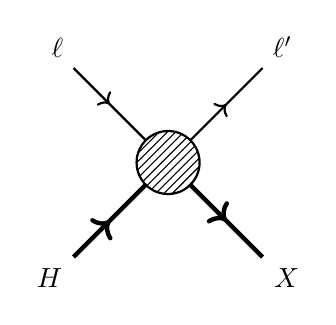
\begin{tikzpicture}[scale=0.8]
\begin{scope}[thick,decoration={
    markings,
    mark=at position 0.5 with {\arrow{>}}}
    ] 
\draw[postaction = {decorate}, ultra thick] (-1.5,-1.5) node[below left]{$H$} -- (-0.35,-0.35);
\draw[postaction = {decorate}] (-1.5,1.5) node[above left]{$\ell$} -- (-0.35,0.35) ;
\draw[postaction = {decorate}, ultra thick] (0.35,-0.35) -- (1.5,-1.5) node[below right]{$X$};
\draw[postaction = {decorate}] (0.35,0.35) -- (1.5,1.5) node[above right]{$\ell'$};
\end{scope}

\fill[pattern=north east lines] circle(0.5cm) (0,0);
\draw[thick] circle(0.5cm) (0,0);
%\draw[thick, snake it] (0,0) -- (1.5,0) node[right]{$B$};
\end{tikzpicture}
\caption{Deep inelastic scattering (DIS) of a lepton $\ell$ on a hadron $H$, producing a lepton $\ell'$ and a hadronic state $X$.}
\label{fig:dis}
\end{figure}

\noindent The differential cross-section for this process, in $d$ spacetime dimensions, may be expressed as:
\begin{align}
\label{eq:diff_xsec_dis}
d\sigma &= \frac{1}{4 \sqrt{(p_{\ell} \cdot p_H)^2 - M_{\ell}^2 M_H^2}} \frac{d^{d-1}\vec{p}_{\ell'}}{(2\pi)^{d-1} 2E_{\ell'}} \sum_{X} \left(\prod_{i=1}^{n_X} \frac{d^{d-1} \vec{p}_{(i,X)}}{(2\pi)^{d-1} 2E_{(i,X)}}\right) \notag \\[1.5ex]
& \qquad\qquad \cdot (2\pi)^d \delta^d\left(p_\ell + p_H - p_{\ell'} - \sum_{i=1}^{n_X} p_{(i,X)}\right) \overline{\left| \mathcal{M}(\ell H \rightarrow \ell' X) \right|^2},
\end{align}
where the pair $(i,X)$ denotes the $i$th particle in the hadronic state $X$ (with $i$ in the range $i \in \{1,...,n_X\}$, for a total of $n_X$ particles in the state $X$), the four-vector $p_{P} = (E_{P}, \vec{p}_{P})$ is the four-momentum of the particle $P$, and $\mathcal{M}(\ell H \rightarrow \ell' X)$ is the amplitude for the process. The sum over $X$ indicates a sum over all possible hadronic states which can be produced in the collision, reflecting our desire to be blind towards the hadronic products. The bar over the modulus-squared amplitude denotes the spin/colour-sum/average; more precisely, we average over the possible spin/colour states of the initial states, and sum over the spin/colour states of the final states (note that for hadronic states $H,X$ the colour sum/average is trivial because hadronic states are colourless). The notation $M_{P}$ means the rest mass of the state $P$.

\begin{figure}[H]
\centering
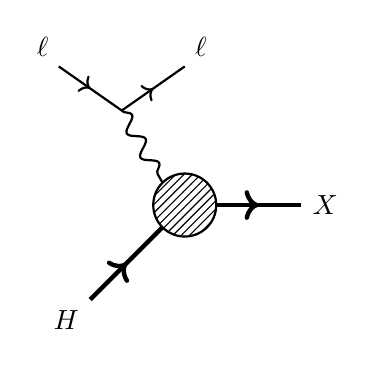
\begin{tikzpicture}[scale=0.8]
\begin{scope}[thick,decoration={
    markings,
    mark=at position 0.5 with {\arrow{>}}}
    ] 
\draw[postaction = {decorate}, ultra thick] (-1.5,-1.5) node[below left]{$H$} -- (-0.35,-0.35);
\draw[postaction = {decorate}, ultra thick] (0.5,0) -- (1.85,0) node[right]{$X$};

\draw[postaction = {decorate}] (-2,2.2) node[above left]{$\ell$} -- (-1,1.5) ;
\draw[postaction = {decorate}] (-1,1.5) -- (0,2.2) node[above right]{$\ell$};
\end{scope}

\fill[pattern=north east lines] circle(0.5cm) (0,0);
\draw[thick] circle(0.5cm) (0,0);
\draw[thick, snake it] (-1,1.5) -- (-0.35,0.35);
\end{tikzpicture}
\caption{Feynman diagram for DIS of an electron off a proton, mediated by a photon, to leading order in QED.}
\label{fig:photondis}
\end{figure}

For ease of exposition, let us now focus on the specific case where $\ell, \ell'$ are electrons, $H$ is a proton, and the process is mediated by a photon. The Feynman diagram for this process (working to leading order in QED for the photon-electron interactions) takes the form shown in Fig.~\ref{fig:photondis}. Thus, the amplitude may be expressed in the form:
\begin{equation}
\mathcal{M}(\ell H \rightarrow \ell'X) = (ie)^2 \bar{u}(p_{\ell'}) \gamma^{\mu} u(p_{\ell}) \cdot \frac{i}{q^2} \cdot \braket{X | J_{\mu} | H},
\end{equation}
where the factors of $ie$ arises from the electron-photon and electron-hadron interactions, the spinor algebra $\bar{u}(p_{\ell'}) \gamma^{\mu} u(p_{\ell})$ arises from the electron lines, the factor of $i/q^2$ comes from the photon propagator (where we have defined $q = p_{\ell} - p_{\ell'}$ to be the momentum of the virtual photon), and the matrix element $\braket{X | J_{\mu} | H}$ comes from the hadron-photon interaction in the lower half of the diagram. Here, $J_{\mu}$ is the electromagnetic current governing photon-quark interactions, given by:
\begin{equation}
J_{\mu} = \sum_{q} e_q \bar{q} \gamma_{\mu} q,
\end{equation}
where $e_q$ is the charge on a quark of flavour $q$, in units of the electron charge. Taking the spin/colour-sum/average of the modulus-squared amplitude, we obtain:
\begin{equation}
\overline{|\mathcal{M}(\ell H \rightarrow \ell'X)|^2} = \frac{e^4}{2q^4} \textrm{Tr}\left( \gamma^{\mu} \slashed{p}_{\ell} \gamma^{\nu} \slashed{p}_{\ell'} \right) \overline{\braket{H | J_{\nu}^{\dagger} | X}\braket{X | J_{\mu} | H}},
\end{equation}
where the bar over the amplitude denotes the spin/colour-sum/average. At this point, it is convenient to introduce two tensors in terms of which the differential cross-section can be parametrised. We define the \textit{leptonic tensor} via:
\begin{equation}
\label{eq:leptonic_tensor}
L^{\mu\nu} = e^4 \textrm{Tr}\left(  \gamma^{\mu} \slashed{p}_{\ell} \gamma^{\nu} \slashed{p}_{\ell'} \right) = 4e^4 \left( p_{\ell}^{\mu} p_{\ell'}^{\nu} + p_{\ell}^{\nu} p_{\ell'}^{\mu} - \eta^{\mu\nu} p_{\ell} \cdot p_{\ell'} \right),
\end{equation}
where the second form is obtained through basic gamma matrix identities, and the \textit{hadronic tensor} via:
\begin{align}
\label{eq:hadronic_tensor}
H_{\mu\nu} &= \frac{1}{4\pi} \sum_{X} \left(\prod_{i=1}^{n_X} \frac{d^{d-1} \vec{p}_{(i,X)}}{(2\pi)^{d-1} 2E_{(i,X)}}\right) \cdot (2\pi)^d \delta^d\left(p_\ell + p_H - p_{\ell'} - \sum_{i=1}^{n_X} p_{(i,X)}\right)  \overline{\braket{H | J_{\nu}^{\dagger} | X}\braket{X | J_{\mu} | H}}.
\end{align}
The differential cross-section may then be expressed in the simplified form:
\begin{equation}
\label{eq:almost_final_dis}
d\sigma = \frac{1}{4\sqrt{(p_{\ell} \cdot p_H)^2 - M_{\ell}^2 M_H^2}} \cdot \frac{1}{q^4} \frac{d^{d-1}\vec{p}_{\ell'}}{(2\pi)^{d-2} 2E_{\ell'}} L^{\mu\nu} H_{\mu\nu}.
\end{equation}
This form is particularly useful, since it clearly decomposes the differential cross section's dependence into a \textit{perturbative} part, namely the leptonic tensor, and a \textit{non-perturbative} part, namely the hadronic tensor. Hence, we have isolated the key challenge in computing a DIS cross-section: modelling the hadronic tensor.

Before commenting further on the hadronic tensor though, it is useful to perform some further superficial work to make Eq.~\eqref{eq:almost_final_dis} match with standard expressions in the literature (see for example Chapter 19 of Ref.~\cite{ParticleDataGroup:2022pth}). We begin by introducing the standard Lorentz-invariant kinematical variables $Q^2$, $x$ and $y$, defined by:
\begin{equation}
\label{eq:dis_kinematics}
Q^2 = -q^2, \qquad x = -\frac{q^2}{2q \cdot p_H}, \qquad y = \frac{q \cdot p_H}{p_{\ell} \cdot p_H}.
\end{equation}
The first invariant quantity is simply the \textit{virtuality} of the mediating photon; it has units of squared energy. The second invariant quantity is called the \textit{Bjorken-$x$}, and its interpretation will become clear when we discuss the parton model shortly. The third invariant quantity is called the \textit{inelasticity}, and measures the fraction of energy lost by the electron; we can see this by working in the rest frame of the hadron, $\vec{p}_H = \vec{0}$, which yields:
\begin{equation}
y = \frac{E_{\ell} - E_{\ell'}}{E_{\ell}} = 1 - \frac{E_{\ell'}}{E_{\ell}},
\end{equation}
where $E_{\ell}$ is the energy of the initial electron, and $E_{\ell'}$ is the energy of the final electron.

Working in four dimensions, $d=4$, we can change variables from $\vec{p}_{\ell'}$ in Eq.~\eqref{eq:almost_final_dis} via:
\begin{align}
d^{3} \vec{p}_{\ell'} &= |\vec{p}_{\ell'}|^{2} d|\vec{p}_{\ell'}| d\cos(\theta) d\phi = |\vec{p}_{\ell'}|^{2}\left|\det\left(\frac{\partial (|\vec{p}_{\ell'}|, \cos(\theta))}{\partial(x, y)}\right) \right| dx dy d\phi,
\label{eq:change_of_variables}
\end{align}
where $\theta$ is the angle defined by $\cos(\theta) := \vec{p}_{\ell} \cdot \vec{p}_{\ell'} / |\vec{p}_{\ell}| |\vec{p}_{\ell'}|$, and $d\phi$ is the remaining angular integral. To calculate the Jacobian matrix in Eq.~\eqref{eq:change_of_variables}, consider working in the rest frame of the proton, so that $\vec{p}_H = \vec{0}$. Then, assuming the masslessness of the electrons so that $E_{\ell} = |\vec{p}_{\ell}|$, $E_{\ell'} = |\vec{p}_{\ell'}|$, we can rewrite the variables in Eq.~\eqref{eq:dis_kinematics} through:
\begin{equation}
\label{eq:change_of_variables}
x = \frac{|\vec{p}_{\ell}| |\vec{p}_{\ell'}| \left(1 - \cos(\theta)\right)}{M_H (|\vec{p}_{\ell}| - |\vec{p}_{\ell'}|)}, \qquad y = 1 - \frac{|\vec{p}_{\ell'}|}{|\vec{p}_{\ell}|},
\end{equation}
where $M_H$ is the rest mass of the proton. Solving these equations simultaneously for $|\vec{p}_{\ell'}|$ and $\cos(\theta)$, we have:
\begin{equation}
|\vec{p}_{\ell'}| = |\vec{p}_{\ell}|(1-y), \qquad \cos(\theta) = 1 - \frac{M_H xy}{|\vec{p}_{\ell}|(1-y)}.
\end{equation}
This allows us to compute the Jacobian factor:
\begin{equation}
\left|\det\left(\frac{\partial (|\vec{p}_{\ell'}|, \cos(\theta))}{\partial(x, y)}\right) \right| = \frac{M_H y}{1-y}.
\end{equation}
Hence the measure in Eq.~\eqref{eq:change_of_variables} may be rewritten as:
\begin{equation}
d^{3} \vec{p}_{\ell'} =  |\vec{p}_{\ell}|^2 (1-y) M_H y \ dx dy d\phi.
\end{equation}
Putting everything together, the differential cross-section Eq.~\eqref{eq:almost_final_dis} may be written in the simple form:
\begin{equation}
\frac{d^3\sigma}{dx dy d\phi} = \frac{y}{32 \pi^2 Q^4} L^{\mu\nu} H_{\mu\nu}.
\end{equation}
To make further progress, we study the Lorentz structure of the hadronic tensor. As can be observed from the definition in Eq.~\eqref{eq:hadronic_tensor}, the only momenta on which the hadronic tensor can depend are the momentum of the initial hadron, $p_H$, and the difference in momentum between the outgoing and ingoing electron, $q$; that is, $H_{\mu\nu} \equiv H_{\mu\nu}(p_H, q)$. The only Lorentz scalars which can be constructed from $p_H$ and $q$ are $p_H^2 = M_H^2$, which is a fixed constant, $q^2 = -Q^2$ and $p_H \cdot q = Q^2/2x$. It can then be shown (see e.g. Ref.~\cite{Halzen:1984mc}) that current conservation at the hadronic vertex implies that the most general Lorentz-covariant structure for the hadronic tensor is given by:
\begin{equation}
H_{\mu\nu}(p_H, q) \equiv \left( -\eta_{\mu\nu} + \frac{q_{\mu} q_{\nu}}{q^2} \right) F_1(x,Q^2) + \left( p_{H\mu} - \frac{p_H \cdot q}{q^2} q_{\mu} \right) \left( p_{H\nu} - \frac{p_H \cdot q}{q^2} q_{\nu} \right) \frac{F_2(x,Q^2)}{p_H \cdot q},
\end{equation}
for some scalar functions $F_1, F_2$, called the \textit{neutral current DIS structure functions}.

Contracting with the expression for the leptonic tensor, Eq.~\eqref{eq:leptonic_tensor},\footnote{When performing this contraction, it is convenient to note that $q_{\mu} L^{\mu\nu} = 0$, by four-momentum conservation.} we arrive at the following expression for the differential cross-section:
\begin{equation}
\frac{d^3\sigma}{dx dy d\phi} = \frac{2y \alpha^2}{Q^4} \left( 2(p_{\ell} \cdot p_{\ell'}) F_1 + \frac{1}{p_H \cdot q} [2 (p_H \cdot p_{\ell}) (p_H \cdot p_{\ell'}) - M_H^2 (p_{\ell} \cdot p_{\ell'})] F_2 \right),
\end{equation}
where $\alpha = e^2 / 4\pi$ is the fine structure constant of QED. To finish, we note that Eq.~\eqref{eq:dis_kinematics} allow us to write:
\begin{equation}
p_{\ell} \cdot p_{\ell'} = \frac{Q^2}{2}, \qquad p_H \cdot p_{\ell} = \frac{Q^2}{2xy}, \qquad p_H \cdot p_{\ell'} = \frac{Q^2}{2x} \left( \frac{1}{y} - 1 \right). 
\end{equation}
Overall then, we can re-express the differential cross-section as:
\begin{equation}
\frac{d^3\sigma}{dx dy d\phi} = \frac{2\alpha^2}{xy Q^2} \left(xy^2F_1 + \left[1 - y - M_H^2 \frac{x^2y^2}{Q^2}\right] F_2\right).
\end{equation}
We see that the right hand side possesses no dependence on the angular variable $\phi$, so may be integrated directly to yield:
\begin{framed}
\begin{equation}
\frac{d^2\sigma}{dx dy} = \frac{4\pi\alpha^2}{xy Q^2} \left(xy^2F_1 + \left[1 - y - M_H^2 \frac{x^2y^2}{Q^2}\right] F_2 \right).
\end{equation}
\end{framed}
This is the final form for the (photon-mediated) DIS differential cross-section, in agreement with Eq. (19.8) of Ref.~\cite{ParticleDataGroup:2022pth}. It is written in terms of the structure functions, $F_1, F_2$, which are the experimentally accessible observables; modelling the hadronic tensor therefore provides predictions for the observable quantities in DIS.


\subsection{The parton model}
So far, the hadronic tensor remains incalculable in perturbation theory, since it depends on the non-perturbative proton state $\ket{H}$. In order to model it, Feynman proposed a phenomenological model called the \textit{parton model}, which we describe as follows. 

It was originally argued in \cite{Feynman:1969wa} that at ultra-relativistic energies (namely in the \textit{deep inelastic limit} $Q^2 \rightarrow \infty$, where the energy transferred from the electron to the proton through the virtual photon approaches infinity), relativistic time-dilation results in the interactions in the proton happening over a characteristic scale $O(1/Q)$. In particular, this implies that at the moment of collision, the impacting electron will interact with only a \textit{single} constituent of the proton. This suggests adopting the following phenomenological model, called the \textit{parton model}, for the hadronic tensor:
\begin{align}
\label{eq:parton_model_hadronic_tensor}
H_{\mu\nu} &= \frac{1}{4\pi} \sum_{q} \int\limits_{0}^{1} \frac{d\xi}{\xi} \sum_{X} \left(\prod_{i=1}^{n_X} \frac{d^{d-1} \vec{p}_{(i,X)}}{(2\pi)^{d-1} 2E_{(i,X)}}\right) \cdot (2\pi)^d \delta^d\left(p_\ell + \xi p_H - p_{\ell'} - \sum_{i=1}^{n_X} p_{(i,X)}\right)\notag \\[1.5ex]
&\qquad\qquad\qquad\qquad \cdot \overline{\braket{q(\xi p_H) | J_{\nu}^{\dagger} | X}\braket{X | J_{\mu} | q(\xi p_H) }} f_q(\xi),
\end{align}
Here, we have replaced the hadronic state $\ket{H}$ with a state $\ket{q(\xi p_H)}$; this denotes a state comprising a free constituent $q$ of the proton,\footnote{Note we also denote the virtuality of the mediating photon by $q$; this should cause no confusion as they enter in different ways.} carrying a fraction $\xi$ of the momentum of the proton $H$. We sum over all possible constituents $q$, and we weight the contributions by some unknown, non-perturbative probability distributions $f_q(\xi)$; these distributions represent the probability of the proton ejecting a constituent $q$ to interact with the electron, carrying a momentum fraction $\xi$. Naturally, we also integrate over all possible momentum fractions. The bar over the amplitude product denotes the spin/colour-sum/average, as usual.

With this assumption on the form of the hadronic tensor, we may calculate the hadronic tensor at lowest order in QCD perturbation theory. In this case, we may take $\ket{X}$ to be a single quark state $\ket{X} = \ket{q(p_X)}$;\footnote{Recall that $X$ was initially defined to be a hadronic state; however, since we are summing over all hadronic states by completeness we may choose to use a basis of quarks and gluons rather than a basis of hadrons, similar to the discussion given around Eqs.~\eqref{eq:completeness} and \eqref{eq:e+e-_completeness}.} then, the hadronic tensor reduces to:
\begin{align}
H_{\mu\nu}^{\text{LO}} &= \frac{1}{2} \sum_{q} \int\limits_{0}^{1} \frac{d\xi}{\xi} \int\frac{d^{d-1} \vec{p}_X}{ 2E_{X}} \delta^d\left(p_\ell + \xi p_H - p_{\ell'} - p_X\right)  \overline{\braket{q(\xi p_H) | J_{\nu}^{\dagger} | q(p_X)}\braket{q(p_X) | J_{\mu} | q(\xi p_H) }} f_q(\xi).
\end{align}
Note that in this case, the colour sum/average of the amplitude product is trivial, since the quark does not change colour during the interaction. The phase space integral can be manipulated via:
\begin{equation}
\int\frac{d^{d-1} \vec{p}_X}{ 2E_{X}} \delta^d\left(p_\ell + \xi p_H - p_{\ell'} - p_X\right) = \int d^d p_X \delta(p_X^2) \delta^d\left( p_{\ell} + \xi p_H - p_{\ell'} - p_X \right),
\end{equation}
which results in:
\begin{align}
H_{\mu\nu}^{\text{LO}} &= \frac{1}{2} \sum_{q}\int\limits_{0}^{1} \frac{d\xi}{\xi}\ \delta((q + \xi p_H)^2) \cdot \ \overline{\braket{q(\xi p_H) | J_{\nu}^{\dagger} | q(q + \xi p_H)}\braket{q(q + \xi p_H) | J_{\mu} | q(\xi p_H) }} f_q(\xi).
\end{align}
In the deep inelastic limit $Q^2 \rightarrow \infty$, corresponding to very high energy transfer from the electron to the proton, we have that $(q + \xi p_H)^2 = q^2 + 2 \xi q \cdot p_H + p_H^2 \approx q^2 + 2 \xi q \cdot p_H$, and hence the delta function condition can be rewritten as:
\begin{equation}
\delta(q^2 + 2 \xi q \cdot p_H) = \frac{\delta(x - \xi)}{2 q \cdot p_H},
\end{equation}
where $x$ is the Bjorken-$x$ we introduced earlier in the text; this reveals that, at leading order in QCD perturbation theory, the interpretation of the Bjorken-$x$ is the momentum fraction carried by the quark state ejected by the hadron which participates in the interaction with the photon. It follows that the hadronic tensor may be expressed in the parton model as:
\begin{align}
H_{\mu\nu}^{\text{LO}} &= \frac{1}{4 x q \cdot p_H} \sum_{q} \overline{\braket{q(x p_H) | J_{\nu}^{\dagger} | q(q + x p_H)}\braket{q(q + x p_H) | J_{\mu} | q(x p_H) }} f_q(x).
\end{align}
We can now straightforwardly compute the matrix elements to yield:
\begin{align}
&\overline{\braket{q(x p_H) | J_{\nu}^{\dagger} | q(q + x p_H)}\braket{q(q + x p_H) | J_{\mu} | q(x p_H) }} \notag\\
&\qquad= \frac{1}{2} e_q^2 \textrm{Tr}(x \slashed{p}_H \gamma_{\nu} (\slashed{q} + x \slashed{p}_H) \gamma_{\mu}) \\[1.5ex]
&\qquad = 2x e_q^2 \left( p_{H\nu} (q + x p_H)_{\mu} + p_{H\mu} (q + x p_H)_{\nu} - \eta_{\mu\nu} p_H \cdot (q + x p_H) \right),\notag
\end{align}
where $e_q$ is the charge on the quark $q$ in units of the electric charge $e$. Note the factor of $1/2$ coming from averaging the ejected quark spin states.

In the ultra-relativistic limit, it becomes appropriate to neglect the mass of the target proton, $M_H^2 \approx 0$; in this case, we can project the structure functions out of the hadronic tensor via the following contractions:
\begin{align}
\label{eq:hadronic_to_structure1}
F_1(x,Q^2) &=\left( -\frac{1}{2} \eta^{\mu\nu} + \frac{2x^2}{Q^2} p_H^{\mu} p_H^{\nu} \right) H_{\mu\nu} (p_H, q), \\[1.5ex]
\label{eq:hadronic_to_structure2}
F_2(x,Q^2) &= \left( - x \eta^{\mu\nu} + \frac{12x^3}{Q^2} p_H^{\mu} p_H^{\nu} \right) H_{\mu\nu}(p_H, q).
\end{align}
Applying the projectors, Eq.~\eqref{eq:hadronic_to_structure1} and Eq.~\eqref{eq:hadronic_to_structure2}, we obtain the following formulae for the structure functions (to leading order in QCD):
\begin{framed}
\begin{align}
F_1^{\text{LO}}(x,Q^2) &= \frac{1}{2}\sum_{q} e_q^2 f_q(x), \\[1.5ex]
F_2^{\text{LO}}(x,Q^2) &= x \sum_{q} e_q^2 f_q(x).
\end{align}
\end{framed}
Note the following important features of our final structure function formulae in the parton model:
\begin{enumerate}[label = (\arabic*)]
\item We have the relation $F_2^{\text{LO}} = 2x F_1^{\text{LO}}$. This identity is called the \textit{Callan-Gross relation}, and provides evidence that the primary constituents of the proton have spin-$\frac{1}{2}$; if we assume different spins for the constituents of the proton, and attempt to perform the calculations presented in this section, we obtain different relations between $F_1^{\text{LO}}, F_2^{\text{LO}}$ which are not observed experimentally (indeed one obtains $F_1^{\text{LO}}\equiv 0$ for scalar quarks, for example - see the discussion below Eq.~(4.18) in \cite{Ellis:1996mzs}). The Callan-Gross relation is not \textit{perfect}; deviations from this law are due to QCD corrections to the parton model, which we shall now discuss.
\item The structure functions are independent of $Q^2$; this is called \textit{Bjorken scaling}, and is experimentally observed when $Q^2 \rightarrow \infty$ (see for example Fig. 6 of Ref.~\cite{Martin:1994kn}). Similarly, Bjorken scaling is broken by QCD corrections to the parton model.
\end{enumerate}

\subsection{The QCD-improved parton model}
We can extend the parton model by including next-to-leading order QCD corrections. The diagrams which contribute to the next-to-leading order QCD corrections can be classified into two categories:
\begin{enumerate}[label = (\roman*)]
\item \textbf{Real and virtual gluon emission.} In this case, a gluon is emitted from either the initial quark leg, or the final quark leg (shown on the left and right of Fig.~\ref{fig:real_gluon_emission} respectively). We take the final state to be $\ket{X} = \ket{q(p_q) g(p_g)}$, comprising a quark of four-momentum $p_q$ and a gluon of four-momentum $p_g$.

Alternatively, a virtual gluon can be emitted from the initial or final quark leg and \textit{reabsorbed}, rather than radiated. We will not give the details of the calculation of these diagrams for brevity, merely stating the results (we shall see that an important cancellation occurs between the real and virtual diagram contributions).

\item \textbf{Gluon-boson fusion.} In this case, a gluon is ejected from the proton, splitting into two quarks; one of the quarks is radiated, whilst the other participates in an interaction with the photon (see Fig.~\ref{fig:gluon_boson_fusion}). Again, in the interest of being brief, we will not give the details of this calculation, simply stating the complete results at the end of the discussion.
\end{enumerate}

\begin{figure}
\centering
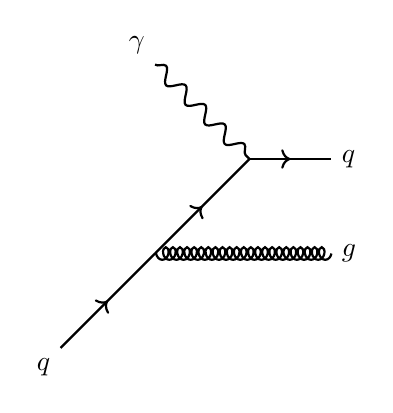
\begin{tikzpicture}[scale=0.8]
\begin{scope}[thick,decoration={
    markings,
    mark=at position 0.5 with {\arrow{>}}}
    ] 
\draw[postaction = {decorate}, thick] (-1.5,-1.5) node[below left]{$q$} -- (0,0);
\draw[postaction = {decorate}, thick] (0,0) -- (1.5,1.5);
\draw[postaction = {decorate}, thick] (1.5,1.5) -- (2.8,1.5) node[right]{$q$};
\end{scope}

%\fill[pattern=north east lines] circle(0.5cm) (0,0);
%\draw[thick] circle(0.5cm) (0,0);
\draw[thick, snake it] (0,3) node[above left]{$\gamma$} -- (1.5,1.5);
\draw[decoration={aspect=0.7, segment length=0.9mm, amplitude=0.8mm,coil}, decorate, thick] (2.8,0) node[right]{$g$} -- (0,0);
\end{tikzpicture}
\hspace{3cm}
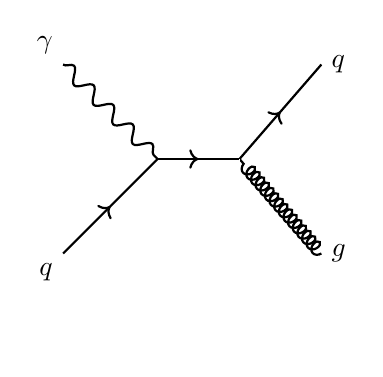
\begin{tikzpicture}[scale=0.8]
\begin{scope}[thick,decoration={
    markings,
    mark=at position 0.5 with {\arrow{>}}}
    ] 
%\draw[postaction = {decorate}, thick] (-1.5,-1.5) node[below left]{$q$} -- (0,0);
\draw[postaction = {decorate}, thick] (0,0) node[below left]{$q$} -- (1.5,1.5);
\draw[postaction = {decorate}, thick] (1.5,1.5) -- (2.8,1.5);
\draw[postaction = {decorate}, thick] (2.8,1.5) -- (4.1,3) node[right]{$q$};
\end{scope}

%\fill[pattern=north east lines] circle(0.5cm) (0,0);
%\draw[thick] circle(0.5cm) (0,0);
\draw[thick, snake it] (0,3) node[above left]{$\gamma$} -- (1.5,1.5);
\draw[decoration={aspect=0.7, segment length=0.9mm, amplitude=0.8mm,coil}, decorate, thick] (4.1,0) node[right]{$g$} -- (2.8,1.5);
\draw[color=white] (2.8,1.5) -- (2.8,-1.5);
\end{tikzpicture}
\caption{\textbf{Left.} Real gluon emission from the initial quark. \textbf{Right.} Real gluon emission from the final quark.}
\label{fig:real_gluon_emission}
\end{figure}

\begin{figure}
\centering
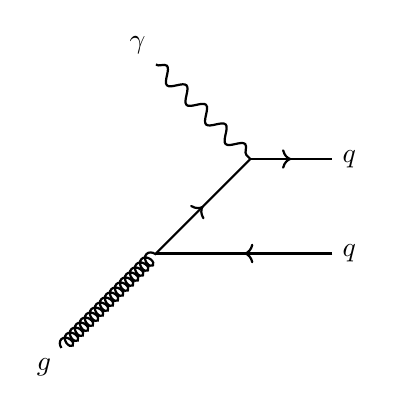
\begin{tikzpicture}[scale=0.8]
\begin{scope}[thick,decoration={
    markings,
    mark=at position 0.5 with {\arrow{>}}}
    ] 
\draw[postaction = {decorate}, thick] (2.8,0) node[right]{$q$} -- (0,0);
\draw[postaction = {decorate}, thick] (0,0) -- (1.5,1.5);
\draw[postaction = {decorate}, thick] (1.5,1.5) -- (2.8,1.5) node[right]{$q$};
\end{scope}

%\fill[pattern=north east lines] circle(0.5cm) (0,0);
%\draw[thick] circle(0.5cm) (0,0);
\draw[thick, snake it] (0,3) node[above left]{$\gamma$} -- (1.5,1.5);
\draw[decoration={aspect=0.7, segment length=0.9mm, amplitude=0.8mm,coil}, decorate, thick] (-1.5,-1.5) node[below left]{$g$} -- (0,0);
\end{tikzpicture}
\caption{Ejection of a gluon from the proton, splitting into a quark which participates in the hard reaction with the photon, and a quark which is radiated. There is also a similar diagram involving antiquarks, where the arrows on the fermion lines are reversed.}
\label{fig:gluon_boson_fusion}
\end{figure}

We begin by computing the contribution to the hadronic tensor from (i), specifically focussing on real gluon emission. Throughout we work in $d$ dimensions, so that we may employ dimensional regularisation when subsequently regulating the theory (we shall find that there are divergences in the calculation). The amplitudes for the diagrams in Fig.~\ref{fig:real_gluon_emission} are, respectively:
\begin{align}
\mathcal{M}_{\mu}^i &= -i g_S \mu^{\epsilon} e_q \bar{u}(p_{q}) \gamma_{\mu} \frac{1}{\xi \slashed{p}_H - \slashed{p}_{g}}\slashed{\epsilon}(p_{g}) t^A u(\xi p_H)  \\[1.5ex]
\mathcal{M}_{\mu}^f &= -i g_S \mu^{\epsilon} e_q \bar{u}(p_q) \slashed{\epsilon}(p_g) \frac{1}{\slashed{p}_q + \slashed{p}_g} \gamma_{\mu} t^A u(\xi p_H),
\end{align}
where $g_S\mu^{\epsilon}$ is the coupling constant of QCD in $d$ dimensions; this is the $d$-dimensional version of the coupling $g_S$ appearing in Eq.~\eqref{eq:qcd_derivative}, but now includes an additional factor of $\mu^{\epsilon}$ where $\mu$ is an arbitrary mass scale and $\epsilon = \frac{4 - d}{2}$. The polarisation of the gluon is given by $\epsilon_{\mu}(p_g)$. The factor of $t^A$ denotes the relevant colour matrix from the Lie algebra $\mathfrak{su}_{\mathbb{C}}(3)$; technically this implies that $\mathcal{M}_{\mu}^i$ should also carry an $SU(3)$-index $A$ corresponding to the colour state of the emitted gluon, but we will suppress this given that we will shortly sum/average over colours. The labels $i,f$ on the respective amplitudes denote a gluon emitted from the \textit{i}nitial quark and the \textit{f}inal quark.

In this case, the contribution to the hadronic tensor is given by:
\begin{align}
\label{eq:hadronic_nlo_real}
H_{\mu\nu}^{\text{NLO, real}} &= \frac{1}{4\pi} \sum_{q} \int\limits_{0}^{1} \frac{d\xi}{\xi} f_q(\xi) \int \frac{d^{d-1} \vec{p}_{q}}{(2\pi)^{d-1} 2E_{q}}  \frac{d^{d-1} \vec{p}_{g}}{(2\pi)^{d-1} 2E_{g}} \notag\\[1.5ex]
&\qquad\qquad\cdot (2\pi)^d \delta^d\left(q + \xi p_H - p_q - p_g\right) \cdot \sum_{r,s=i,f} \overline{\mathcal{M}_{\mu}^r \mathcal{M}_{\nu}^{s\dagger}} ,
\end{align}
where, as usual, the bar on the amplitude product denotes the spin/colour-sum/average. This expression can be evaluated in two steps: first, we will manipulate the phase space into a more amenable form, and then second, we shall compute the spin/colour-sum/averages of the amplitude products.

We begin by noting that:
\begin{align}
&\int \frac{d^{d-1} \vec{p}_{q}}{(2\pi)^{d-1} 2E_{q}}  \frac{d^{d-1} \vec{p}_{g}}{(2\pi)^{d-1} 2E_{g}} \cdot (2\pi)^d \delta^d\left(q + \xi p_H - p_q - p_g\right) \notag\\[1.5ex]
&\qquad= \frac{1}{2(2\pi)^{d-2}} \int  \frac{d^{d-1} \vec{p}_{g}}{E_{g}} d^d p_q\ \delta(p_q^2) \delta^d\left(q + \xi p_H - p_q - p_g\right)\notag\\[1.5ex]
&\qquad= \frac{1}{2(2\pi)^{d-2}} \int \frac{d^{d-1} \vec{p}_{g}}{E_{g}} \delta( (q + \xi p_H - p_g)^2) 
\end{align}
To absorb the remaining delta function, we make a sequence of variable changes. Consider first changing variables from $\vec{p}_g$ to $(|\vec{p}_g|^2, \cos(\theta))$, where $\theta$ is the angle defined by:
\begin{equation}
\cos(\theta) = \frac{\vec{p}_g \cdot \xi \vec{p}_H}{|\vec{p}_g| |\xi \vec{p}_H|} = \frac{\vec{p}_g \cdot \vec{p}_H}{|\vec{p}_g| |\vec{p}_H|}.
\end{equation}
The measure transforms as:\footnote{Recall the gluon is real, so on-shell, and hence $E_g = |\vec{p}_g|$.}
\begin{align}
\int \frac{d^{d-1} \vec{p}_g}{E_g} &= \frac{1}{2} \int |\vec{p}_g|^{d-4} \sin^{d-4}(\theta) d(|\vec{p}_g|^2) d(\cos(\theta)) d\Omega_{d-3}\notag \\[1.5ex]
&= \frac{(d-2) \pi^{\frac{1}{2}(d-2)}}{2\Gamma(d/2)} \int  |\vec{p}_g|^{d-4} \sin^{d-4}(\theta) d(|\vec{p}_g|^2) d(\cos(\theta)) \notag\\[1.5ex]
&= \frac{\pi^{1-\epsilon}}{\Gamma(1-\epsilon)} \int  |\vec{p}_g|^{d-4} \sin^{d-4}(\theta) d(|\vec{p}_g|^2) d(\cos(\theta)),
\end{align}
where $d\Omega_{d-3}$ contains all angular integrations in $d-3$ dimensions, except for the integration over $\theta$; in the second line we perform the integration over $d\Omega_{d-3}$ using a standard hyperspherical integral, and in the final line we recall that $d = 4 - 2\epsilon$.

We now make a second change of variables. Consider introducing the variables $u,v$ defined by the conditions:
\begin{equation}
\label{eq:soft_and_collinear_definitions}
p_g \cdot p_q = \frac{Q^2}{2} \left( \frac{1-u}{u} \right), \qquad p_g \cdot \xi p_H = \frac{Q^2 v}{2u}.
\end{equation}
The interpretation of these variables will become clear shortly. In order to relate the variables $u,v$ to the variables $|\vec{p}_g|^2$, $\cos(\theta)$, we work in the centre of momentum frame where $\vec{q} + \xi \vec{p}_H = \vec{0} = \vec{p}_g + \vec{p}_q$. The four-vectors $q, \xi p_H, p_g, p_q$ can then be expressed as:
\begin{equation}
q = \begin{pmatrix} \sqrt{\xi^2 |\vec{p}_H|^2 - Q^2} \\ -\xi \vec{p}_H \end{pmatrix}, \quad \xi p_H = \begin{pmatrix} \xi |\vec{p}_H| \\ \xi \vec{p}_H  \end{pmatrix}, \quad p_g = \begin{pmatrix} |\vec{p}_g| \\ \vec{p}_g \end{pmatrix}, \quad p_q = \begin{pmatrix} |\vec{p}_g| \\ -\vec{p}_g \end{pmatrix},
\end{equation}
where the first component of the virtual photon's four-momentum can be computed by enforcing the condition $q^2 = -Q^2$. Using the definition of $u$ from $p_g \cdot p_q$, and working in the above frame, we see that:
\begin{equation}
|\vec{p}_g|^2 = \frac{Q^2}{4} \left( \frac{1-u}{u} \right).
\end{equation}
In particular, we see that $u$ describes the \textit{energy} of the radiated gluon; in particular, the limit $u \rightarrow 1$ corresponds to the limit in which the energy of the gluon goes to zero, the so-called \textit{soft} limit. 

To obtain a relation between $v$ and $|\vec{p}_g|, \cos(\theta)$, we note that by conservation of energy, we can deduce that:
\begin{equation}
 \sqrt{\xi^2 |\vec{p}_H|^2 - Q^2} + \xi |\vec{p}_H| = 2 |\vec{p}_g| \qquad \Rightarrow \qquad  \xi |\vec{p}_H| = \frac{4 |\vec{p}_g|^2 + Q^2}{4|\vec{p}_g|}.
\end{equation}
Then the definition of $v$ in terms of $p_g \cdot \xi p_H$, we have:
\begin{align}
\frac{Q^2 v}{2u} &= |\vec{p}_g| \xi | \vec{p}_H| - \vec{p}_g \cdot \xi \vec{p}_H \notag\\[1.5ex]
&= |\vec{p}_g| \xi |\vec{p}_H| (1 - \cos(\theta)) \notag\\[1.5ex]
&= \frac{Q^2}{4u}(1 - \cos(\theta)),
\end{align}
which yields:
\begin{equation}
v = \frac{1 - \cos(\theta)}{2}.
\end{equation}
Hence $v$ is a measure of the \textit{collinearity} of the outgoing quark and the radiated gluon; in particular, as $v \rightarrow 0$, we have the outgoing quark and the radiated gluon are collinear.

Computing the Jacobian factor, we can now make the change of variables to $u,v$. We note that:
\begin{equation}
d(|\vec{k}_g|^2) d\cos(\theta) = \frac{\partial(|\vec{k}_g|^2, \cos(\theta))}{\partial(u,v)} du dv = \frac{Q^2}{2u^2} du dv,
\end{equation}
and hence it follows that the phase space can be written in terms of $u, v$ as:
\begin{equation}
\frac{1}{2(2\pi)^{2 - 2\epsilon}} \frac{\pi^{1-\epsilon}}{2\Gamma(1-\epsilon)} Q^{2(1-\epsilon)} \int  du dv\ \frac{(1-u)^{-\epsilon}}{u^{2-\epsilon}} v^{-\epsilon} (1-v)^{-\epsilon} \delta( (q + \xi p_H - p_g)^2).
\end{equation}
To finish, we note that the argument of the delta function can be expanded to:
\begin{equation}
(q + \xi p_H - p_g)^2 = q^2 + 2 q \cdot \xi p_H - 2 q \cdot p_g - 2 \xi p_H \cdot p_g.
\end{equation}
Using Eq.~\eqref{eq:soft_and_collinear_definitions}, we can obtain the missing inner products of four-vectors which we require in evaluating this expression. We find that:
\begin{equation}
(q + \xi p_H - p_g)^2 = \delta\left( Q^2 \left( \frac{1}{u} - \frac{\xi}{x} \right) \right) = \frac{x\delta(\xi - x/u)}{Q^2},
\end{equation}
Using the delta function to absorb the $\xi$ integral in the hadronic tensor, we see that we have reduced the hadronic tensor to:

\begin{align}
\label{eq:hadronic_nlo_real_phase_space}
H_{\mu\nu}^{\text{NLO, real}} &= \frac{1}{4\pi} \sum_{q}\frac{1}{2(2\pi)^{2 - 2\epsilon}} \frac{\pi^{1-\epsilon}}{2\Gamma(1-\epsilon)} Q^{-2\epsilon} \int  du dv\ f_q\left( \frac{x}{u} \right) \frac{(1-u)^{-\epsilon}}{u^{1-\epsilon}} v^{-\epsilon} (1-v)^{-\epsilon} \sum_{r,s=i,f} \overline{\mathcal{M}_{\mu}^r \mathcal{M}_{\nu}^{s\dagger}} \\[1.5ex]
&= \frac{1}{32 \pi ^2 \Gamma(1 - \epsilon)} \left( \frac{4\pi}{Q^2} \right)^{\epsilon} \sum_{q} \int\limits_{x}^{1} \frac{du}{u} f_q\left( \frac{x}{u} \right) \frac{u^{\epsilon}}{(1-u)^{\epsilon}} \int\limits_{0}^{1} dv\ v^{-\epsilon} (1-v)^{-\epsilon} \sum_{r,s=i,f} \overline{\mathcal{M}_{\mu}^r \mathcal{M}_{\nu}^{s\dagger}}.
\label{eq:hadronic_nlo_real_phase_space_2}
\end{align}
The integration ranges can be obtained by considering the allowed regions of $u,v$ arising from their definitions in Eq.~\eqref{eq:soft_and_collinear_definitions}.\\

\noindent It remains to compute the spin/colour-sum/averages of the quantities quadratic in the amplitudes, $\overline{\mathcal{M}_{\mu}^r \mathcal{M}_{\nu}^{s\dagger}}$. Here, we shall only compute $\overline{\mathcal{M}_{\mu}^i \mathcal{M}_{\nu}^{i\dagger}}$ to demonstrate the details of such a calculation; the others can be obtained by similar means. We begin by observing that:
\begin{equation}
\label{eq:nlo_amplitude_squared}
\overline{\mathcal{M}_{\mu}^i \mathcal{M}_{\nu}^{i\dagger}} = \frac{e_q^2 g_S^2 \mu^{2\epsilon} C_F}{2(\xi p_H - p_g)^4} g^{\alpha\beta}_{\perp}(k_g) \textrm{Tr}\left( \slashed{p}_q \gamma_{\mu} (\xi \slashed{p}_H - \slashed{p}_g) \gamma_{\alpha} \xi \slashed{p}_H \gamma_{\beta} (\xi \slashed{p}_H - \slashed{p}_g) \gamma_{\nu} \right).
\end{equation}
The trace arises from the usual method of taking spin-sum/averages of spinors. The factor of $C_F = 4/3$ arises from the colour-sum/averages; in particular, it is the quadratic Casimir of $\mathfrak{su}_{\mathbb{C}}(3)$, obeying:
\begin{equation}
\sum_{A} (t^A)^2 = C_F I.
\end{equation}
Finally, the factor of $g^{\alpha\beta}_{\perp}(k_g)$ arises from the spin-sum/average of the radiated gluon; it is given by:
\begin{equation}
g^{\alpha\beta}_{\perp}(k_g) := \sum_{\text{polarisations}} \epsilon^{\alpha}(k_g) \epsilon^{\beta*}(k_g).
\end{equation} 
The sum depends on which polarisations are allowed in the final state. To simplify things as much as possible, we shall assume that \textit{all} polarisations are allowed, including unphysical ones. This requires us to also consider the introduction of ghost fields; however, fortunately at this order in QCD there are no diagrams which include the ghosts. Therefore, we can happily conclude that:
\begin{equation}
g^{\alpha\beta}_{\perp}(k_g) = \sum_{\text{polarisations}} \epsilon^{\alpha}(k_g) \epsilon^{\beta*}(k_g) = \eta^{\alpha\beta},
\end{equation}
the standard result when all polarisations are considered. This allows us to reduce Eq.~\eqref{eq:nlo_amplitude_squared} to the simplified form:
\begin{align}
\overline{\mathcal{M}_{\mu}^i \mathcal{M}_{\nu}^{i\dagger}} &= \frac{e_q^2 g_S^2 \mu^{2\epsilon} C_F}{8(\xi p_H \cdot k_g)^2} \textrm{Tr}\left( \slashed{p}_q \gamma_{\mu} (\xi \slashed{p}_H - \slashed{p}_g) \gamma_{\alpha} \xi \slashed{p}_H \gamma^{\alpha} (\xi \slashed{p}_H - \slashed{p}_g) \gamma_{\nu} \right)\notag\\[1.5ex]
&= \frac{2 (1-\epsilon) e_q^2 g_S^2 \mu^{2\epsilon} C_F}{\xi p_H \cdot p_g}  \left( \eta_{\mu\nu} p_g \cdot p_q - (p_g)_{\mu} (p_q)_{\nu} - (p_g)_{\nu} (p_q)_{\mu}\right),
\end{align}
where the trace can be evaluated by standard Dirac algebra methods.\footnote{Note that in the case where a $Z$-boson or a $W$-boson mediates deep inelastic scattering, rather than a photon, these traces additionally contain $\gamma^5$ matrices. The definition of $\gamma^5$ in $d = 4 - 2\epsilon$ dimensions is rather subtle, and a lot more care is required in these calculations. A detailed discussion can be found in \cite{Collins:1984xc}.} The factor of $1-\epsilon$ arises from a contraction of the form $\eta^{\alpha\beta} \eta_{\alpha\beta} = d = 4 - 2\epsilon$, recalling that we are working in $d = 4-2\epsilon$ dimensions.

Evaluating the other spin/colour-sum/averages of the quantities quadratic in the amplitudes, it can be shown that we have the following projections:
\begin{align}
-\eta^{\mu\nu} \sum_{r,s=i,f} \overline{\mathcal{M}_{\mu}^r \mathcal{M}_{\nu}^{s\dagger}} &= 4 e_q^2 g_S^2 \mu^{2\epsilon} C_F (1-\epsilon) \left[ (1-\epsilon) \left( \frac{p_g \cdot p_q}{p_g \cdot \xi p_H} + \frac{p_g \cdot \xi p_H}{p_g \cdot p_q}\right) + \frac{Q^2 (\xi p_H \cdot p_q)}{(p_g \cdot \xi p_H) (p_g \cdot p_q)} + 2\epsilon\right],\\[1.5ex]
p_H^{\mu} p_H^{\nu} \sum_{r,s=i,f} \overline{\mathcal{M}_{\mu}^r \mathcal{M}_{\nu}^{s\dagger}} &= \frac{4 e_q^2 g_S^2 \mu^{2\epsilon} C_F (1-\epsilon)}{\xi^2} (p_q \cdot \xi p_H).
\end{align}
These projections can be rewritten conveniently in terms of the `softness' and `collinearity' variables $u,v$ we introduced in Eq.~\eqref{eq:soft_and_collinear_definitions}:
\begin{align}
-\eta^{\mu\nu} \sum_{r,s=i,f} \overline{\mathcal{M}_{\mu}^r \mathcal{M}_{\nu}^{s\dagger}} &= 4 e_q^2 g_S^2 \mu^{2\epsilon} C_F (1-\epsilon) \left[ (1-\epsilon) \left( \frac{1-u}{v} + \frac{v}{1-u}\right) + \frac{2u(1-v)}{v(1-u)} + 2\epsilon\right],\\[1.5ex]
p_H^{\mu} p_H^{\nu} \sum_{r,s=i,f} \overline{\mathcal{M}_{\mu}^r \mathcal{M}_{\nu}^{s\dagger}} &= \frac{2 e_q^2 g_S^2 \mu^{2\epsilon} C_F (1-\epsilon) Q^2 (1-v) u}{x^2}.
\end{align}
Inserting these formulae into the appropriate projections of Eq.~\eqref{eq:hadronic_nlo_real_phase_space_2}, we obtain:
\begin{align}
\label{eq:real_transverse_unsimplified}
-\eta^{\mu\nu} H_{\mu\nu}^{\text{NLO, real}} &= \frac{\alpha_S C_F  (1-\epsilon)}{2\pi \Gamma(1 - \epsilon)} \left( \frac{4\pi \mu^2}{Q^2} \right)^{\epsilon} \sum_{q} e_q^2 \int\limits_{x}^{1} \frac{du}{u} f_q\left( \frac{x}{u} \right) \frac{u^{\epsilon}}{(1-u)^{\epsilon}} \notag\\[1.5ex]
& \qquad\qquad \cdot \int\limits_{0}^{1} dv\ v^{-\epsilon} (1-v)^{-\epsilon}  \left[ (1-\epsilon) \left( \frac{1-u}{v} + \frac{v}{1-u}\right) + \frac{2u(1-v)}{v(1-u)} + 2\epsilon\right],\\[1.5ex]
p^{\mu}_H p^{\nu}_H H_{\mu\nu}^{\text{NLO, real}} &=\frac{\alpha_S Q^2 C_F (1-\epsilon)}{4\pi x^2 \Gamma(1 - \epsilon)} \left( \frac{4\pi \mu^2}{Q^2} \right)^{\epsilon} \sum_{q} e_q^2 \int\limits_{x}^{1} \frac{du}{u} f_q\left( \frac{x}{u} \right) \frac{u^{1 + \epsilon}}{(1-u)^{\epsilon}} \int\limits_{0}^{1} dv\ v^{-\epsilon} (1-v)^{1-\epsilon},
\end{align}
where $\alpha_S = g_S^2 / 4\pi$ is the strong coupling. We wish to determine the behaviour of these expressions as $\epsilon \rightarrow 0$, i.e. as we restore $d=4$ dimensions. We note that the projection $p^{\mu}_H p^{\nu}_HH_{\mu\nu}^{\text{NLO, real}}$ remains finite in this limit, giving the result:
\begin{equation}
p^{\mu}_H p^{\nu}_H H_{\mu\nu}^{\text{NLO, real}} =\frac{\alpha_S Q^2 C_F}{8\pi x^2} \sum_{q} e_q^2 \int\limits_{x}^{1} du f_q\left( \frac{x}{u} \right).
\end{equation}
On the other hand, the projection $-\eta^{\mu\nu} H_{\mu\nu}^{\text{NLO, real}}$ is singular as $\epsilon \rightarrow 0$, and requires a more careful treatment. To begin with, we note that we can evaluate the collinear $v$ integral using the identity:\footnote{Technically this result holds only when $\Re(p), \Re(q) > 0$, but we can always pretend that $\epsilon$ is an appropriate range before using analytic continuation to justify whichever final result we get.}
\begin{equation}
\int\limits_{0}^{1} dv\ v^{p-1} (1-v)^{q-1} = \frac{\Gamma(p)\Gamma(q)}{\Gamma(p+q)}.
\end{equation} 
Applying this result repeatedly, we can simplify Eq.~\eqref{eq:real_transverse_unsimplified} to:
\begin{align}
&-\eta^{\mu\nu} H_{\mu\nu}^{\text{NLO, real}} = \frac{\alpha_S C_F  (1-\epsilon)}{2\pi \Gamma(1 - \epsilon)} \left( \frac{4\pi \mu^2}{Q^2} \right)^{\epsilon} \sum_{q} e_q^2 \int\limits_{x}^{1} \frac{du}{u} f_q\left( \frac{x}{u} \right) \frac{u^{\epsilon}}{(1-u)^{\epsilon}} \notag\\[1.5ex]
& \ \cdot \left[ (1-\epsilon) \left(  \frac{(1-u)\Gamma(-\epsilon)\Gamma(1-\epsilon)}{\Gamma(1 - 2\epsilon)} +  \frac{\Gamma(2 - \epsilon) \Gamma(1-\epsilon)}{(1-u)\Gamma(3 - 2\epsilon)} \right) + \frac{2u}{1-u} \frac{\Gamma(-\epsilon)\Gamma(2-\epsilon)}{\Gamma(2 - 2\epsilon)} + 2\epsilon \frac{\Gamma(1-\epsilon)^2}{\Gamma(2-2\epsilon)} \right],
\end{align}
which by repeated application of the functional equation of the gamma function, $\Gamma(x+1) = x\Gamma(x)$, may be reduced to the more convenient form:
\begin{align}
-\eta^{\mu\nu} H_{\mu\nu}^{\text{NLO, real}} &= \frac{\alpha_S C_F  (1-\epsilon) \Gamma(1-\epsilon)}{2\pi \Gamma(1 - 2\epsilon)} \left( \frac{4\pi \mu^2}{Q^2} \right)^{\epsilon} \sum_{q} e_q^2 \int\limits_{x}^{1} \frac{du}{u} f_q\left( \frac{x}{u} \right) \frac{u^{\epsilon}}{(1-u)^{\epsilon+1}} \notag\\[1.5ex]
&\qquad \cdot \left[ \left( -\frac{1}{\epsilon} + 1\right)(1-u)^2 +  \frac{1-\epsilon}{2(1-2\epsilon)} - \frac{2u(1-\epsilon)}{\epsilon(1-2\epsilon)} + \frac{2\epsilon}{1 - 2\epsilon} \right].
\label{eq:collinear_singularity}
\end{align}
We must now Laurent expand this formula in small $\epsilon$. The key result we shall require is:
\begin{equation}
\label{eq:plus_identity}
\frac{u^{\epsilon}}{(1-u)^{\epsilon+1}} = -\frac{1}{\epsilon} \delta(1-u) + \left( \frac{1}{1-u} \right)_+ - \epsilon \left( \frac{\log(1-u)}{1-u} \right)_+ + \epsilon \frac{\log(u)}{1-u} + O(\epsilon^2),
\end{equation}
which holds only in a distributional sense.\footnote{That is, when integrated against a smooth function from $u=0$ to $u=1$.} A proof of this identity is given in App.~\ref{app:plus_prescription}. Here, the $+$ symbol denotes the \textit{plus distribution}, defined by:
\begin{equation}
\int\limits_{0}^{1} F(u)_+ G(u)\ du = \int\limits_{0}^{1} F(u)(G(u) - G(1))\ du.
\end{equation}
Combining the identity Eq.~\eqref{eq:plus_identity} with the standard Laurent expansions of the rational function expression in the large square brackets, as $\epsilon \rightarrow 0$ we see that the projection $-\eta^{\mu\nu} H_{\mu\nu}^{\text{NLO, real}}$ behaves as:
\begin{align}
&-\eta^{\mu\nu} H_{\mu\nu}^{\text{NLO, real}} = \frac{\alpha_S C_F  (1-\epsilon) \Gamma(1-\epsilon)}{2\pi \Gamma(1 - 2\epsilon)} \left( \frac{4\pi \mu^2}{Q^2} \right)^{\epsilon} \sum_{q} e_q^2 \int\limits_{x}^{1} \frac{du}{u} f_q\left( \frac{x}{u} \right) \bigg[ \left( \frac{2}{\epsilon^2} + \frac{3}{2\epsilon} + \frac{7}{2} \right) \delta(1-u) \notag\\[1.5ex]
&\qquad- \frac{1}{\epsilon} \frac{1 + u^2}{(1-u)_+} + 3 - u - \frac{3}{2(1-u)_+} + (1+u^2) \left( \frac{\log(1-u)}{1-u} \right)_+ - \frac{1+u^2}{1-u} \log(u) + O(\epsilon)\bigg].
\end{align}
We see that there is a double pole as $\epsilon \rightarrow 0$; the origin of this can be traced back to the soft singularity as $u\rightarrow 1$ (this is made manifest in Eq.~\eqref{eq:plus_identity}), combined with the collinear singularity as $v \rightarrow 0$ (this is made manifest in Eq.~\eqref{eq:collinear_singularity}, since after we have performed the $v$ integration, we obtain a $1/\epsilon$ term).\\

\noindent We must sum the real gluon emissions with the virtual gluon emissions, which enter at the same order in QCD, and multiply the same quark distributions $f_q(\xi)$ in the parton model for the hadronic tensor. The calculation of these diagrams is equally long and arduous,\footnote{Though it is possible to use some physical arguments to reduce the workload, see e.g. the discussion around Eq.~(4.70) of Ref.~\cite{Ellis:1996mzs}.} so we shall merely state the complete results here. We find that in the limit as $\epsilon \rightarrow 0$, we obtain the contribution:
\begin{align}
\label{eq:virtual_transverse_unsimplified}
-\eta^{\mu\nu} H_{\mu\nu}^{\text{NLO, virtual}} &= -\frac{\alpha_S C_F  (1-\epsilon) \Gamma(1-\epsilon)}{2\pi \Gamma(1 - 2\epsilon)} \left( \frac{4\pi \mu^2}{Q^2} \right)^{\epsilon} \sum_{q} e_q^2 \int\limits_{x}^{1} \frac{du}{u} f_q\left( \frac{x}{u} \right) \delta(1-u) \notag\\[1.5ex]
& \qquad\qquad\qquad\qquad\qquad \cdot \left( \frac{2}{\epsilon^2} + \frac{3}{\epsilon} + 8 + \frac{\pi^2}{3} + O(\epsilon)\right)
\end{align}
with $p^{\mu}_H p^{\nu}_H H_{\mu\nu}^{\text{NLO, virtual}}$ vanishing as $\epsilon \rightarrow 0$. We note that the double pole, the $O(\epsilon^{-2})$ term, is cancelled exactly between the real and virtual corrections.\\

%\noindent The calculation of the second class of diagrams, namely the gluon-initiated gluon-boson fusion diagrams (ii), proceeds similarly and, for brevity, we omit the details of the calculation in this thesis. We obtain the following projections in this case, in the limit as $\epsilon \rightarrow 0$:
%\begin{align}
%-\eta^{\mu\nu} H_{\mu\nu}^{\text{NLO, gluon}} &= \frac{\alpha_S T_R (1-\epsilon) \Gamma(1-\epsilon)}{\pi \Gamma(1-2\epsilon)} \left( \frac{4 \pi \mu^2}{Q^2} \right)^{\epsilon} \sum_{q} e_q^2 \int\limits_{x}^{1} \frac{du}{u} f_g\left( \frac{x}{u} \right) \notag   \\[1.5ex]
%\label{eq:gluon_transverse_unsimplified}
%&\quad \cdot \left[ -\frac{1}{\epsilon} (1 + u - u^2) - (1 + u - u^2) \log\left( \frac{u}{1-u} \right) + O(\epsilon) \right],\\[1.5ex]
% \label{eq:gluon_longitudinal_unsimplified}
%p^{\mu}_H p^{\nu}_H H_{\mu\nu}^{\text{NLO, gluon}} &= \frac{\alpha_S Q^2 T_R}{2x^2 \pi}  \sum_{q} e_q^2 \int\limits_{x}^{1} du\  f_g\left( \frac{x}{u} \right) (1-u) ,
%\end{align}
%where $T_R = 1/2$ is the Casimir of $\mathfrak{su}_{\mathbb{C}}(3)$ in the adjoint representation. Again, the projection $p^{\mu}_H p^{\nu}_H H_{\mu\nu}^{\text{NLO, gluon}}$ is finite in the limit as $\epsilon \rightarrow 0$.\\

\noindent Putting everything together then, we obtain the following complete formulae for the projections of the quark-initiated part of the hadronic tensor at next-to-leading order in QCD perturbation theory:
\begin{framed}
\begin{align}
\label{eq:full_nlo_transverse_unsimplified}
&-\eta^{\mu\nu} H_{\mu\nu}^{\text{quark, LO+NLO}} = \sum_{q} e_q^2 f_q(x) + \frac{\alpha_S C_F (1-\epsilon) \Gamma(1-\epsilon)}{2\pi \Gamma(1-2\epsilon)} \left( \frac{4\pi \mu^2}{Q^2} \right)^{\epsilon} \sum_{q} e_q^2 \int\limits_{x}^{1} \frac{du}{u} \notag \\[1.5ex]
&\qquad\qquad\qquad\qquad\quad \cdot f_q\left( \frac{x}{u} \right)\bigg[ \left( -\frac{3}{2\epsilon} - \frac{\pi^2}{3} - \frac{9}{2} \right) \delta(1-u) - \frac{1}{\epsilon} \frac{1 + u^2}{(1-u)_+} + 3 - u \notag \\[1.5ex]
&\qquad\qquad\qquad\qquad\quad - \frac{3}{2(1-u)_+} + (1+u^2) \left( \frac{\log(1-u)}{1-u} \right)_+ - \frac{1+u^2}{1-u} \log(u) \bigg], \\[1.5ex]
&p_H^{\mu} p_H^{\nu} H_{\mu\nu}^{\text{quark, LO+NLO}} = \frac{\alpha_S C_F Q^2}{8\pi x^2}  \sum_{q} e_q^2 \int\limits_{x}^{1} du\ f_q\left( \frac{x}{u} \right).
\end{align}
\end{framed}
\noindent Rather disturbingly, we have discovered that in the limit $\epsilon \rightarrow 0$, the hadronic tensor in the parton model at next-to-leading order in QCD appears to be \textit{singular}, corresponding to a collinear divergence from the real gluon emission that has not been cancelled with the divergence arising from the virtual gluon emission. It is at this point that the distributions $f_{q}(\xi)$ begin their starring role. 

\subsection{Definition of the $\overline{\text{MS}}$ PDFs} 
We initially introduced $f_q(\xi)$ as a probability distribution, representing the probability of a quark of momentum fraction $\xi$ being ejected from the proton and participating in the interaction with the photon. However, just as in the process of ultraviolet renormalisation, we can instead drop this interpretation beyond the leading order,\footnote{Just as the `bare mass' in a QFT Lagrangian no longer has the interpretation of mass beyond tree level.} and instead view these distributions as `bare theory parameters', subsequently renormalising them to absorb the leftover collinear divergences. In particular, this can be effected by allowing the `bare distributions' $f_q(\xi)$ to have an $\epsilon$ dependence, $f_q(\xi) \equiv f_q(\xi,\epsilon)$. If the bare distribution $f_q(\xi,\epsilon)$ is divergent as $\epsilon \rightarrow 0$, then it is no longer necessary that the hadronic tensor projection in Eq.~\eqref{eq:full_nlo_transverse_unsimplified} is singular as $\epsilon \rightarrow 0$, since the divergences may now cancel one another. 

Hence, with a view to redefining the `bare distributions' $f_q(x,\epsilon)$ to absorb all divergences in Eq.~\eqref{eq:full_nlo_transverse_unsimplified}, let us make the definition:
\begin{framed}
\begin{equation}
\label{eq:pdf_definition}
f_q^{\overline{\text{MS}}}(x, \mu_F^2) := f_q(x,\epsilon) - \frac{\alpha_S}{2\pi} \int\limits_{x}^{1} \frac{du}{u} f_q\left( \frac{x}{u},\epsilon\right) P_{qq}(u) \left( \frac{1}{\epsilon} - \log\left( \frac{\mu_F^2}{\mu^2} \right) - \gamma + \log(4\pi) \right),
\end{equation}
\end{framed}
\noindent where $\gamma$ is the Euler-Mascheroni constant,\footnote{Which appears in the Taylor expansion $\Gamma(1+x) = 1 - \gamma x + O(x^2)$ about $x=0$.} and $P_{qq}(u)$ is called the \textit{quark-quark splitting function}\footnote{Whilst the standard name is \textit{function}, $P_{qq}(u)$ is technically a \textit{distribution}, and only makes sense when integrated against a smooth function.} defined by:
\begin{equation}
P_{qq}(u) := C_F \left[ \frac{3}{2} \delta(1-u) + \frac{1+u^2}{(1-u)+} \right].
\end{equation} 
\noindent The new object we have defined here is called the \textit{modified minimal subtraction NLO quark parton distribution function} (which we shall henceforth refer to simply as an NLO \textit{parton distribution function} (NLO PDF), or even just PDF when the order is implied; no other subtraction scheme will be considered in this thesis). It is a renormalised version of the `bare PDF' $f_q(x,\epsilon)$. The term `modified minimal subtraction' refers to this redefinition purely absorbing the collinear divergence, i.e. the pole term of order $O(1/\epsilon)$, plus the universal terms $-\gamma$, $\log(4\pi)$, which come from the expansion of the gamma function and the power law $(4\pi Q^2/\mu^2)^{\epsilon}$.

This redefinition allows us to rewrite the projection $-\eta^{\mu\nu} H_{\mu\nu}^{\text{quark, LO+NLO}}$ as:
\begin{align}
&-\eta^{\mu\nu} H_{\mu\nu}^{\text{quark, LO+NLO}} = \sum_{q} e_q^2 f_{q}^{\overline{\text{MS}}}(x, \mu_F^2) + \frac{\alpha_S C_F }{2\pi} \sum_{q} e_q^2 \int\limits_{x}^{1} \frac{du}{u}\ f_q^{\overline{\text{MS}}}\left( \frac{x}{u},\mu_F^2 \right) \cdot \bigg[ \frac{P_{qq}(u)}{C_F} \log\left( \frac{Q^2}{\mu_F^2} \right)\notag\\[1.5ex]
\label{eq:final_hadronic_transverse}
&  - \left(  \frac{\pi^2}{3} + \frac{9}{2} \right) \delta(1-u) + 3 - u - \frac{3}{2(1-u)_+} + (1+u^2) \left( \frac{\log(1-u)}{1-u} \right)_+ - \frac{1+u^2}{1-u} \log(u) \bigg] + O(\alpha_S^2), 
\end{align}
\noindent which is now finite in the limit as $\epsilon \rightarrow 0$. The parameter $\mu_F^2$ in the parton distributions is referred to as the \textit{factorisation scale}, and controls the finite part which is absorbed by the redefinition along with the singular part, which is of course arbitrary. However, it is customary to take $\mu_F^2 = Q^2$ to cancel any large logarithmic contribution coming from the first term in the NLO contribution of Eq.~\eqref{eq:final_hadronic_transverse}.

We also note that the parton distributions $f_q^{\overline{\text{MS}}}(x,\mu_F^2)$ are themselves now finite in the limit as $\epsilon \rightarrow 0$; since the projection $-\eta^{\mu\nu} H_{\mu\nu}^{\text{quark, LO+NLO}}$ is physical and hence finite, and all the functions that the PDF multiplies on the right hand side of Eq.~\eqref{eq:final_hadronic_transverse} are now finite, it follows that $f_q^{\overline{\text{MS}}}(x,\mu_F^2)$ must be finite too. This implies a cancellation between the divergent behaviour of the bare PDF $f_q(x,\epsilon)$ as $\epsilon \rightarrow 0$ and the collinear pole $1/\epsilon$ as $\epsilon \rightarrow 0$ (at least at this order in perturbation theory in $\alpha_S$).

\subsection{Complete results for the NLO DIS structure functions}
Combining with the gluon-initiated diagrams (ii), and allowing for a slightly more involved redefinition of $f_q, f_g$ which now involves quark-gluon mixing, we obtain final expressions for the hadronic tensor at next-to-leading order in QCD perturbation theory. When the structure functions are finally projected out using Eq.~\eqref{eq:hadronic_to_structure1} and Eq.~\eqref{eq:hadronic_to_structure2}, we obtain the final results:
\begin{align}
F_2^{\text{LO+NLO}} &= x \sum_{q} e_q^2 \int\limits_{x}^{1} \frac{du}{u}\ f^{\overline{\text{MS}}}_q\left(\frac{x}{u},\mu_F^2\right)   \bigg( \delta(1-u) + \frac{\alpha_S}{2\pi} P_{qq}(u) \log\left( \frac{Q^2}{\mu_F^2} \right) \notag\\[1.5ex]
&\qquad\qquad\qquad + \frac{\alpha_S C_F}{2\pi} \left[ \frac{1+u^2}{1-u} \left( \frac{\log(1-u)}{u} - \frac{3}{4} \right) + \frac{5u + 9}{4}\right]_+\bigg) \notag \\[1.5ex]
&\quad + x \sum_{q} e_q^2 \int\limits_{x}^{1} \frac{du}{u}\ f^{\overline{\text{MS}}}_g\left( \frac{x}{u}, \mu_F^2\right) \frac{\alpha_S}{2\pi} \bigg( P_{qg}(u) \log\left( \frac{Q^2}{\mu_F^2}\right) \notag \\[1.5ex]
&\qquad\qquad\qquad + T_R \left[ (u^2 + (1-u)^2) \log\left( \frac{1-u}{u} \right) - 1 + 8u(1-u)\right] \bigg),\\[1.5ex]
F_1^{\text{LO+NLO}} &= \frac{1}{2x} F_2^{\text{LO+NLO}} - \frac{\alpha_S}{2\pi} \sum_{q} e_q^2 \int\limits_{x}^{1} \frac{du}{u} \left( C_F f_q^{\overline{\text{MS}}}\left( \frac{x}{u} \right) u + 4T_R f_g^{\overline{\text{MS}}} u(1-u) \right).
\end{align}
where the splitting function $P_{qg}(u)$ is defined by:
\begin{equation}
P_{qg}(u) := T_R ( u^2 + (1-u)^2 ),
\end{equation}
with $T_R=1/2$ a Casimir of a further $\mathfrak{su}_\mathbb{C}(3)$ representation, and where for compactness we have applied the distributional identity:
\begin{align}
&-\left( \frac{\pi^2}{3} + \frac{9}{2} \right) \delta(1-u) + 3 + 2u - \frac{3}{2(1-u)_+} + (1+u^2) \left( \frac{\log(1-u)}{1-u} \right)_+ - \frac{1+u^2}{1-u} \log(u)\notag \\[2ex]
&\qquad\qquad\qquad\qquad\qquad\qquad\qquad\qquad \equiv \left[ \frac{1+u^2}{1-u} \left( \frac{\log(1-u)}{u} - \frac{3}{4} \right) + \frac{5u + 9}{4}\right]_+,
\end{align}
which is proved in App.~\ref{app:plus_prescription}. We can further simplify notation by introducing the \textit{Mellin convolution}:
\begin{equation}
(f \otimes g)(x) := \int\limits_{x}^{1} \frac{du}{u} f(u) g\left( \frac{x}{u} \right) = \int\limits_{x}^{1} \frac{du}{u} f\left( \frac{x}{u} \right) g(u),
\end{equation}
in terms of which the final next-to-leading order structure function formulae can be written as:
\begin{framed}
\begin{align}
\label{eq:structure_function_factorisation_2}
F_2^{\text{LO+NLO}} &=\sum_{q} \hat{F}_2^{q,\text{LO+NLO}} \otimes f_q^{\overline{\text{MS}}} + \hat{F}_2^{g,\text{LO+NLO}} \otimes f_g^{\overline{\text{MS}}} \\[1.5ex]
\label{eq:structure_function_factorisation_1}
F_1^{\text{LO+NLO}} &= \frac{1}{2x} F_2^{\text{LO+NLO}} - \frac{\alpha_S}{2\pi} \sum_{q} e_q^2 \left( C_F f_q^{\overline{\text{MS}}} \otimes u + 4T_R f_g^{\overline{\text{MS}}} \otimes u(1-u) \right),
\end{align}
where we have the `partonic' structure function expressions:
\begin{align}
\hat{F}_2^{q,\text{LO+NLO}} &= xe_q^2 \bigg( \delta(1-u) + \frac{\alpha_S}{2\pi} P_{qq}(u) \log\left( \frac{Q^2}{\mu_F^2} \right)\notag \\[1.5ex]
&\qquad + \frac{\alpha_S C_F}{2\pi} \left[ \frac{1+u^2}{1-u} \left( \frac{\log(1-u)}{u} - \frac{3}{4} \right) + \frac{5u + 9}{4}\right]_+\bigg), \\[1.5ex]
\hat{F}_2^{g,\text{LO+NLO}} &= \frac{x\alpha_S}{2\pi} \bigg( P_{qg}(u) \log\left( \frac{Q^2}{\mu_F^2}\right) \notag \\[1.5ex]
&\qquad + T_R \left[ (u^2 + (1-u)^2) \log\left( \frac{1-u}{u} \right) - 1 + 8u(1-u)\right] \bigg).
\end{align}
\end{framed}
\noindent In particular, Eq.~\eqref{eq:structure_function_factorisation_2} and Eq.~\eqref{eq:structure_function_factorisation_1} are of the `factorisation theorem' form described in Eq.~\eqref{eq:generic_factorisation_theorem}, where in this case we have a single PDF and no fragmentation functions. Whilst we have not rigorously \textit{proved} factorisation (some notes on various ways in which this can be achieved are given at the end of this section), the work we have done in constructing Eqs.~\eqref{eq:structure_function_factorisation_2} and \eqref{eq:structure_function_factorisation_1} lends credence to the idea that factorisation is true.

\subsection{Universality of PDFs}
Before concluding this section with a discussion of how factorisation theorems can be rigorously \textit{proved}, we make an important remark regarding the \textit{universality} of the PDFs constructed in this section. 

Whilst the NLO $\overline{\text{MS}}$ PDFs we defined in this section were introduced in a study of DIS, their definition actually applies in a wide variety of processes where hadrons are present in the initial state. Indeed, we can see this from the definition Eq.~\eqref{eq:pdf_definition}, since the only part that relied on any amplitude calculation was the \textit{splitting function} $P_{qq}(u)$. Furthermore, the part of the amplitude calculation that goes into the computation of the splitting function $P_{qq}(u)$ can be shown to be independent of the fact we are studying DIS; indeed, it can be shown (see e.g. the discussion in Altarelli and Parisi's famous paper, Ref.~\cite{Altarelli:1977zs}) to be the probability that a quark radiates a collinear quark and a collinear gluon, with the quark carrying a fraction $u$ of the initial quark's momentum. This applies similarly to the splitting function $P_{qg}(u)$ we defined above; in general, we can construct splitting functions $P_{ij}(u)$ whose interpretation is the probability that a parton of type $j$ emits a collinear parton of type $i$, with momentum fraction $u$ of the original parton (possibly with other partons as appropriate).

Thus, since the NLO $\overline{\text{MS}}$ PDFs are constructed purely from universal, process-independent objects, they themselves are universal. For example, it can be shown that for the \textit{Drell-Yan process}, $pp \rightarrow \ell^+ \ell^- X$, involving two protons colliding to produce a detected lepton-antilepton pair and any other hadronic state $X$, we obtain the following factorisation theorem for the cross-section:
\begin{equation}
\sigma = \sum_{q_1, q_2} \hat{\sigma} \otimes f_{q_1}^{\overline{\text{MS}}} \otimes f_{q_2}^{\overline{\text{MS}}},
\end{equation} 
where the sum over $q_1, q_2$ is over all proton constituents (including gluons), $\hat{\sigma}$ is the relevant perturbatively-calculable hard cross-section, and $f_{q_i}^{\overline{\text{MS}}}$ are the \textit{same} PDFs we defined in the DIS construction above. This is the great attraction of factorisation theorems - we have packaged all of our ignorance of non-perturbative physics into universal objects which can be deployed in a very wide variety of processes, leaving only the perturbative, hard physics to calculate on a case by case basis.

\subsection{Proofs of factorisation}
Despite the intuitive picture that the parton model and its QCD improvement provide, we have not in any sense \textit{proved} that our factorisation theorem is valid; in the above, we merely introduced a phenomenological model for the hadronic tensor, Eq.~\eqref{eq:parton_model_hadronic_tensor}, essentially conjecturing its form in terms of unknown functions. 

It is possible to rigorously derive the parton model from first principles in QCD, but the proofs are difficult and are beyond the scope of this thesis. In the case of DIS, there is a (somewhat) elementary proof relying on Wilson's \textit{operator product expansion} (OPE), and explained in detail in Chapter 32.4.3 of Ref.~\cite{Schwartz:2014sze}). However, the use of the OPE is limited, and more sophisticated techniques are required for more general processes than DIS.

One of the most successful methods of proving factorisation theorems is the method of Collins, Soper and Sterman (summarised nicely in Ref.~\cite{Collins:1989gx}), which involves showing that the dominant Feynman diagrams for a given process can be organised into a `hard' sub-diagram and a `PDF' sub-diagram (these need not be the case na\"{i}vely - we could have double parton emission, or even more complicated diagrams, hence we must show that such diagrams are negligible\footnote{In fact, they are shown to be suppressed by powers of a characteristic energy scale of the process; these contributions are called \textit{higher twist} in the literature.}). The method is reasonably accessible in the case of a scalar theory, where the hadron is supposed to be built of spin-$0$ constituents (see Chapter 5 of Ref.~\cite{Collins:1989gx} for a full explanation), but in fully-fledged QCD becomes more difficult; the reason is that collinear divergences are also joined by \textit{soft} divergences corresponding to the massless gluons having zero energy - showing that the soft divergences cancel is extremely subtle.

More recently, factorisation theorems have been proved in the \textit{soft-collinear effective field theory} (SCET) approach (see Ref.~\cite{Bauer:2001yt}, for example). This relies on constructing an effective theory of QCD, where the separation of the theory is based on collinearity and softness (rather than in a standard effective theory, which involves integrating out massive particles). We shall have a lot more to say about effective field theories (EFTs) in Chapters~\ref{chap:smeftdy} and~\ref{chap:top}.




\section{Properties of parton distribution functions}
\label{sec:pdfproperties}
Having defined PDFs (at least at NLO in QCD), it will be useful to report some of their salient properties; in this section, we describe some key features of the PDFs which shall be used throughout this thesis. First, we construct the \textit{evolution equations} for parton distributions in the $\overline{\text{MS}}$ scheme; these evolution equations give a perturbative description of the dependence of the the PDFs on the factorisation scale. Second, we state the \textit{valence} and \textit{momentum} sum rules for PDFs. Finally, we comment on two important features of the PDFs: their \textit{positivity}, and their large-$x$ and small-$x$ \textit{scaling} behaviour.

\subsection{Evolution equations}
Consider taking the logarithmic $\mu_F^2$ derivative of Eq.~\eqref{eq:pdf_definition} above. We find that:
\begin{align}
\mu_F^2 \frac{\partial}{\partial \mu_F^2} f_q^{\overline{\text{MS}}}(x,\mu_F^2)& = \frac{\alpha_S}{2\pi} \int\limits_{x}^{1} \frac{du}{u} P_{qq}(u) f_q^{\overline{\text{MS}}}\left( \frac{x}{u}, \mu_F^2\right) + O(\alpha_S^2) \notag \\[1.5ex]
\label{eq:basic_dglap}
&= \frac{\alpha_S}{2\pi} (P_{qq} \otimes f_q^{\overline{\text{MS}}})(x, \mu_F^2) + O(\alpha_S^2).
\end{align}
In particular, we see that the quark parton distribution functions obey an integro-differential equation in their second argument; this equation is called the \textit{Dokshitzer-Gribov-Lipatov-Altarelli-Parisi} (DGLAP) equation \cite{Altarelli:1977zs,Dokshitzer:1977sg,Gribov:1972ri}, and is the analogue of a Callan-Symanzik equation from standard ultraviolet renormalisation. Of course, Eq.~\eqref{eq:basic_dglap} ignores the gluon distribution; if we make the redefinition in Eq.~\eqref{eq:pdf_definition} also including the gluon-initiated diagrams, we must allow for quark-gluon mixing, which leads to the more complete set of DGLAP equations:
\begin{align}
\mu_F^2 \frac{\partial}{\partial \mu_F^2} \begin{pmatrix} f_q^{\overline{\text{MS}}}(x,\mu_F^2) \\ f_g^{\overline{\text{MS}}}(x,\mu_F^2) \end{pmatrix} &= \frac{\alpha_S}{2\pi} \int\limits_{x}^{1} \frac{du}{u} \begin{pmatrix} P_{qq}(u) & P_{qg}(u) \\ P_{gq}(u) & P_{gg}(u) \end{pmatrix}  \begin{pmatrix} f_q^{\overline{\text{MS}}}\left( x/u, \mu_F^2\right) \\ f_g^{\overline{\text{MS}}}\left(x/u, \mu_F^2\right) \end{pmatrix} + O(\alpha_S^2),\\[1.5ex]
\label{eq:qcd_dglap}
&= \frac{\alpha_S}{2\pi} \begin{pmatrix} P_{qq} & P_{qg} \\ P_{gq} & P_{gg} \end{pmatrix}  \otimes \begin{pmatrix} f_q^{\overline{\text{MS}}} \\ f_g^{\overline{\text{MS}}} \end{pmatrix} \left(x , \mu_F^2\right) + O(\alpha_S^2),
\end{align}
where the relevant additional splitting functions are given by:
\begin{align}
P_{gq}(u) &:= C_F \left( \frac{1 + (1-u)^2}{u} \right),\\[1.5ex]
P_{gg}(u) &:= 2 C_A \left( \frac{u}{(1-u)_+} + \frac{1-u}{u} + u(1-u) \right) + \delta(1-u) \frac{(11C_A - 24 T_R)}{6},
\end{align}
with $C_A = 3$ the Casimir of a further representation of $\mathfrak{su}_\mathbb{C}(3)$. As described above, these splitting functions can be determined in a process-independent way; this will be particularly useful in Chapter~\ref{chap:darkphoton}.

It is also important to note that the equations we have presented above are accurate to next-to-leading order in QCD perturbation theory; we can extend these equations using higher order QCD splitting functions, and indeed QED splitting functions, which shall be relevant in Chapter~\ref{chap:darkphoton}. The QCD contributions
to the splitting functions were fully computed up to $O(\alpha_S^3)$
in~\cite{Vogt:2004mw,Moch:2004pa,Blumlein:2021enk},\footnote{They are also partially
  known at $O(\alpha_S^4)$~\cite{Moch:2021qrk}, but this contribution
  are not yet fully known and are not included in any public 
PDF evolution code.} the mixed QED and QCD contribution
was computed in~\cite{deFlorian:2015ujt}, and the NLO QED contribution was computed in~\cite{deFlorian:2016gvk}.

These evolution equations can be solved numerically. Software able to do this includes APFEL (\textbf{A} \textbf{P}D\textbf{F} \textbf{E}volution \textbf{L}ibrary) \cite{Bertone:2013vaa} and EKO (\textbf{E}volution \textbf{K}ernel \textbf{O}perators) \cite{Candido:2022tld}; the former is used throughout the thesis with occasional modification. In both cases, a rotation of PDF flavours is made to simplify the matrix of splitting functions, decoupling some of the evolution equations from one another; more details are presented in \cite{Bertone:2013vaa}, with some further discussion in Chapter~\ref{chap:darkphoton}.

\subsection{Sum rules}
The initial interpretation of the `bare' PDFs as probability distributions implies that they should obey certain `\textit{sum rules}'. In particular, since hadrons are composed of a collection of a fixed number of \textit{valence quarks}, together with particles generated by virtual exchange, we must have:
\begin{equation}
\label{eq:bare_valence_sum_rule}
\int\limits_{0}^{1} dx\ \left( f_q(x) - f_{\bar{q}}(x) \right) = N_q,
\end{equation}
for each of the quarks $q$, where $\bar{q}$ denotes the associated antiquark, and where $N_q$ is the number of valence quarks of type $q$ which form the hadron. In the case of a proton, we have $N_u = 2$ and $N_d = 1$, with $N_q = 0$ for all other flavours of quarks. This relation survives the redefinition of the PDFs, Eq.~\eqref{eq:pdf_definition}, yielding the \textit{valence sum rules}:
\begin{equation}
\label{eq:valence_sum_rule}
\int\limits_{0}^{1} dx\ \left( f_q^{\overline{\text{MS}}}(x, \mu_F^2) - f_{\bar{q}}^{\overline{\text{MS}}}(x,\mu_F^2) \right) = N_q.
\end{equation}
Similarly, the introduction of the PDFs as probability distributions in momentum fraction, $x$, means that we have the \textit{momentum sum rule}:
\begin{equation}
\label{eq:momentum_sum_rule}
\int\limits_{0}^{1} dx\ x \left( \sum_{q} f_q^{\overline{\text{MS}}}(x, \mu_F^2) + f_g^{\overline{\text{MS}}}(x,\mu_F^2) \right) = 1,
\end{equation}
where the sum over $q$ is over all quarks and antiquarks.

These rules are naturally extended to accommodate additional constituents of the proton; for example, if we study the proton at higher order in QED, the momentum sum rule must be adjusted to accommodate a contribution from the \textit{photon} PDF, and the \textit{lepton} PDFs. These considerations will be important in Chapter~\ref{chap:darkphoton}.

\subsection{Positivity}
When we introduced PDFs in Sect.~\ref{sec:factorisation} in the context of the parton model, they were motivated as probability densities describing the probability of ejecting different constituents of the proton carrying different momentum fractions; as such, the `bare' distributions should in principle be \textit{positive} quantities. However, we saw that the inclusion of NLO QCD effects requires a redefinition of these `bare' distributions, given in Eq.~\eqref{eq:pdf_definition}, removing this initial interpretation; therefore, traditionally there has been no expectation for PDFs beyond the leading order to be positive.

However, a proof has recently become available that this is indeed the case \cite{Candido:2020yat}; the proof is beyond the scope of this thesis, but we shall assume its result - namely that for each PDF flavour, we have:
\begin{equation}
f^{\overline{\text{MS}}}(x,\mu_F^2) \geq 0
\end{equation}
for all $x \in [0,1], \mu_F^2 \in [0,\infty)$.\footnote{It is worth noting, however, that the rigour of the proof is somewhat in question; in particular, Ref.~\cite{Collins:2021vke} shows that in fact `bare' PDFs need not be positive in $d = 4 - 2\epsilon$ dimensions, which is a major assumption of the proof in Ref.~\cite{Candido:2020yat}. Nonetheless, the NNPDF fitting collaboration assume positivity of the PDFs, and given that this thesis works closely with their methodology, we shall do the same.}

\subsection{Large-$x$ and small-$x$ behaviour}
\label{sec:pdf_scaling}
Since a constituent of the proton cannot be ejected with momentum fraction $x > 1$, we must have:
\begin{equation}
\lim_{x \rightarrow 1} f^{\overline{\text{MS}}}(x, \mu_F^2) = 0
\end{equation}
for all flavours of PDF. On the other hand, the scaling behaviour of the PDFs in the limit as $x \rightarrow 0$ is also known, dictated by \textit{Regge theory}; in brief, this theory tells us that, quite generally, scattering amplitude are proportional to certain power laws governed by information on the angular momentum of the process. It turns out (see Ref.~\cite{Abarbanel:1969eh}) that this implies the PDFs themselves must obey a power law scaling in the small-$x$ limit:
\begin{equation}
f^{\overline{\text{MS}}}(x,\mu_F^2) \propto x^{\alpha}, \qquad \text{as $x \rightarrow 0$,}
\end{equation}
for each flavour of PDF (though $\alpha$ will depend on the flavour). The upshot of these two scaling limits is that PDFs take the general form:
\begin{equation}
f^{\overline{\text{MS}}}(x,\mu_F^2) = x^{\alpha} (1-x)^{\beta} \tilde{f}(x,\mu_F^2),
\end{equation}
with $\beta > 0$, for some unknown function $\tilde{f}$; this suggests the functional form that most PDF fitting collaborations build upon, as we shall discuss in the subsequent section, Sec.~\ref{sec:pdffitting}.


\section{Fitting parton distribution functions}
\label{sec:pdffitting}

Above, we introduced parton distributions to parametrise the non-perturbative structure of hadrons. Their very definition implies that they cannot be obtained by perturbative methods, which essentially leaves open two options for their determination: (i) lattice methods (see e.g. \cite{Cichy:2019ebf} for some progress in this direction); (ii) fits to experimental data. In this text, we focus exclusively on the latter choice, which we shall describe in detail in this section.

We begin by describing possible functional forms which can be used to model the PDFs. The parameters in these functional forms are obtained by fits to a given dataset by the minimisation of a loss function, namely the $\chi^2$-statistic (in the $t_0$ prescription, with various penalty terms), which we subsequently motivate and define. Next, we describe a method for minimisation of the loss function, namely \textit{stochastic gradient descent}. Finally, we describe a standard method of error analysis in PDF fits, namely the \textit{Monte Carlo replica method}, which allows for the propagation of experimental uncertainties onto the PDFs. 

A discussion of the actual datasets used in PDF fits is deliberately omitted and is deferred to later chapters; different datasets will be used to fit the PDFs for each of the scenarios considered in this text.

\subsection{The choice of functional form}
The space of possible parton distributions is an \textit{infinite}-dimensional function space, comprising solutions of the DGLAP equations, Eq.~\eqref{eq:qcd_dglap}, which obey the momentum and valence sum rules; as such, given only \textit{finite} amounts of data, it is an ill-posed problem to determine the PDFs. Therefore, any PDF fitting attempt must initially restrict the infinite-dimensional PDF space to a \textit{finite}-dimensional space instead, by assuming a functional form for the PDFs. Typically, a functional form is assumed at some initial factorisation scale $Q = Q_0$, below any characteristic energy scale for data entering the fit, and then DGLAP evolution is used to obtain the PDF at all scales. For the modern datasets used by most PDF fitting collaborations, the initial scale for fits is typically taken to be $Q_0 = 1.65$ GeV (as in, say, Ref.~\cite{NNPDF:2021njg}).

Many functional forms are available; to give an early example, in Martin, Stirling and Roberts' analysis of PDFs in 1994~\cite{Martin:1994kn}, the authors choose the following parametrisation for the valence quark distributions and the gluon distribution:\footnote{For brevity, we shall now drop the superscript $\overline{\text{MS}}$ denoting the modified minimal subtraction PDFs; we shall henceforth assume that all PDFs use this scheme.}
\begin{align}
x(f_u - f_{\bar{u}})(x,Q_0^2) &= A_u x^{\eta_1} (1-x)^{\eta_2} (1 + \epsilon_u \sqrt{x} + \gamma_u x),\\
x(f_d - f_{\bar{d}})(x,Q_0^2) &= A_d x^{\eta_3} (1-x)^{\eta_4} (1 + \epsilon_d \sqrt{x} + \gamma_d x),\\
xf_g(x,Q_0^2) &= A_g x^{-\lambda} (1-x)^{\eta_g} (1 + \gamma_g x).
\end{align}
This form is motivated by the known large-$x$ and small-$x$ scaling behaviour of the PDFs, which we described above in Sect.~\ref{sec:pdf_scaling}, supplemented by a polynomial factor in $\sqrt{x}$ (the choice of a polynomial in $\sqrt{x}$ rather than in $x$ is found to give a better fit). The authors also impose certain flavour assumptions, for example that the strange content of the proton is equal to the anti-strange content of the proton ($f_{s} = f_{\bar{s}}$), due to the datasets not being adequately able to disentangle the two.

Fitting groups have since extended this basic functional form and removed flavour assumptions as more data has become available, allowing the PDFs to be determined more precisely. Some modern fitting collaborations, for example the \textit{The Coordinated Theoretical-Experimental Project on QCD} (CTEQ) group, even use an ensemble of functional forms to account for the bias expected by restricting to a particular individual functional form (see Ref.~\cite{Hou:2019efy}, for example).

More recently, the \textit{Neural Network Parton Distribution Function} (NNPDF) collaboration (see Ref.~\cite{NNPDF:2021njg} for their most recent global PDF fit) have parametrised PDFs using neural networks, which shall be the most relevant parametrisation in this thesis. The initial-scale form of the PDFs adopted by NNPDF is given by:
\begin{equation}
xf(x,Q_0^2) = x^{\alpha}(1-x)^{\beta} \text{NN}(x; \vec{w}),
\end{equation}
where $\text{NN}(x; \vec{w})$ is the output of a neural network parametrised by $\vec{w}$ (the details of the architecture, and how it is extended appropriately for this thesis, are given in Sec.~\ref{sec:simunet}), and $\alpha, \beta$ are fixed prior to the fit;\footnote{Technically fixed for each \textit{replica} in the fit individually; see the below discussion of the Monte Carlo replica method of error propagation used by the NNPDF collaboration. On a separate note, it has recently been shown in Ref.~\cite{Carrazza:2021yrg} that the scaling prefactor is not in fact necessary, and the network can learn this behaviour.} the fit is then iterated to check stability of $\alpha, \beta$. The main advantage claimed by NNPDF in using a neural network parametrisation is that it allows the exploration of an extremely large space of functions, removing the bias inherent in fixed functional form approaches. This is supported by so-called `universal approximation theorems' (see Ref.~\cite{HORNIK1989359}, for example), which tell us that any given function can be well-approximated by a sufficiently deep neural network.

\subsection{The loss function}
Once we have decided on a functional form with which to model the PDFs, we must obtain the parameters in the model by the minimisation of a loss function on the global dataset. The natural first-choice for a loss function is the $\chi^2$-statistic, defined by:
\begin{equation}
\label{eq:chi2}
\chi^2(\vec{w}) = (\vec{d} - \vec{t}(\vec{w}))^T \Sigma^{-1} (\vec{d} - \vec{t}(\vec{w})),
\end{equation}
where $\vec{d}$ is the vector of experimental central values, $\vec{t}(\vec{w})$ is the vector of corresponding theory predictions for the experimental datapoints (dependent on the model parameters $\vec{w}$), and $\Sigma$ is the experimental covariance matrix describing correlations between the data. The intuition for this choice of loss function is that we wish the theory predictions to be close to the data, but if the data is more uncertain, we should not require the agreement between data and theory to be as precise. This can be most easily seen in the case that the data is uncorrelated, in which case the covariance matrix is diagonal, and the $\chi^2$-statistic reduces to:
\begin{equation}
\label{eq:chi2_uncorrelated}
\chi^2(\vec{w}) = \sum_{i=1}^{N_{\text{dat}}} \frac{(d_i - t_i(\vec{w}))^2}{\sigma_i^2},
\end{equation}
where $N_{\text{dat}}$ is the total number of datapoints, and $\sigma_i$ is the uncertainty on the $i$th datapoint; when the $i$th datapoint is very uncertain, i.e. $\sigma_i$ is large, we have that the contribution to the $\chi^2$-statistic from the difference between data and theory at the $i$th datapoint is suppressed. The form Eq.~(\ref{eq:chi2}) retains this interpretation in the case that the data is additionally correlated.

\paragraph{Positivity.} It is necessary to make some modifications to this na\"{i}ve loss function in modern PDF fits. Firstly, the requirement that PDFs are positive, described in Sect.~\ref{sec:pdfproperties} above, can be encoded into the loss function through the use of penalty terms:\footnote{In fact, in the NNPDF fits, further penalty terms are also included to ensure that certain benchmark pseudo-observables (called \textit{positivity datasets}) are positive. This is required because positivity of the PDFs does not guarantee positivity of cross-sections, and vice-versa.

Additionally, NNPDF also impose similar penalties ensuring the \textit{integrability} of the PDFs, but we omit the details as the idea is essentially the same.}
\begin{equation}
\chi^2_{\text{pos}}(\vec{w}) = \chi^2(\vec{w}) + \sum_{q} \Lambda_q \sum_{k=1}^{N_{\text{grid}}} \textrm{ELU}_{\alpha}\left( - f_q(x_k, 5 \text{ GeV}^2) \right),  
\end{equation}
as described in Eq. (3.10) of Ref.~\cite{NNPDF:2021njg}. The sum is over all fitted PDF flavours $q$, and $x_1, x_2, ..., x_{N_{\text{grid}}}$ is the $x$-grid on which we demand positivity. The scale $Q^2 = 5 \text{ GeV}^2$ is chosen to be above the charm mass; this is for technical reasons explained in Ref.~\cite{Candido:2020yat}, wherein it is shown that massive quark PDFs need not be positive below their mass threshold. DGLAP evolution preserves positivity beyond the initial chosen positivity scale.

The function $\textrm{ELU}_{\alpha}$ is the \textit{exponential linear unit}, defined by:
\begin{equation}
\textrm{ELU}_{\alpha}(t) = \begin{cases} t, & \text{if $t \geq 0$;} \\ \alpha (e^t - 1), & \text{if $t < 0$,} \end{cases}
\end{equation}
which is intended to penalise negative PDFs but pass positive PDFs (of course other choices of functions would work for this purpose too). The parameters $\Lambda_q$ and $\alpha$ are hyperparameters, which are chosen to maximise fit quality (indeed, in the NNPDF framework, they are chosen by a hyperoptimisation procedure, described in detail in Sec. 3.3 of Ref.~\cite{NNPDF:2021njg} - additionally, the parameters $\Lambda_q$ are increased at each step of the minimisation to improve convergence).

\paragraph{The $t_0$ prescription.} The second modification to the loss function comes from a slightly unexpected place: we must modify the loss function when we have datasets that include multiplicative normalisation uncertainties. A full discussion of why this is the case is given in Ref.~\cite{Ball:2009qv}, but here we give some brief intuition. 

Consider a fit which includes two measurements of the same observable, say $d_1, d_2$ with $d_1 < d_2$. Suppose further that each of these measurements carries an equal multiplicative normalisation uncertainty, $s$; in particular, this implies that the absolute error on $d_1$ is $s d_1$ and the absolute error on $d_2$ is $s d_2$. Now, despite the experimentalists reporting the same error for both datapoints, when minimising the na\"{i}ve $\chi^2$, there will be a bias towards the value $d_1$ since it carries the smaller uncertainty. This bias is called the \textit{d'Agostini bias}, after the author who first introduced it in Ref.~\cite{DAgostini:1993arp}; minimal examples with far greater mathematical detail are presented in Sec. 3.1 of Ref.~\cite{Ball:2009qv}.

The bias can be countered using the so-called \textit{$t_0$ prescription} for the $\chi^2$-statistic, as described in Ref.~\cite{Ball:2009qv}. In brief, this involves the addition of a covariance matrix of theory predictions being added to the usual experimental covariance matrix, modifying it to the so-called $t_0$ covariance matrix, $\Sigma_{t_0}$. The matrix of theory predictions that we add to the covariance matrix depends on a PDF set, called the \textit{$t_0$ PDF set}; however, the dependence on this set is usually weak, and in the NNPDF methodology, fits are \textit{iterated} (that is, a new fit is run using the output of the initial fit as the $t_0$ PDF set) to check stability.

\subsection{Minimisation of the loss function}
To actually perform a PDF fit, we must minimise the chosen loss function through some optimisation method. This is a highly non-trivial task, since the loss function as a function of $\vec{w}$ is typically extremely complicated, with multiple local (possibly degenerate) minima. Various algorithms exist to perform the minimisation; here we shall describe only the standard method used by the NNPDF collaboration, namely \textit{stochastic gradient descent}.\footnote{Although previously NNPDF minimised the loss function by use of a \textit{genetic algorithm}, see Ref.~\cite{NNPDF:2014otw}.} See Ref.~\cite{Carrazza:2019mzf} for the first discussion of the use of gradient descent methods in the NNPDF framework.

\paragraph{Gradient descent.} Before describing stochastic gradient descent, it is useful to describe \textit{deterministic} gradient descent first. The algorithm works as follows. Suppose that we wish to determine a local minimum of the loss function $\chi^2_{t_0+\text{pos}}(\vec{w})$ as a function of the PDF parameters. 

\begin{enumerate}[label = (\arabic*)]
\item Choose some initial values of the PDF parameters, $\vec{w} = \vec{w}_0$. Choose also some value for the \textit{learning rate}, $\gamma$, which should be a positive real number.
\item Given $\vec{w}_n$ for $n=0,1,...$, define $\vec{w}_{n+1} = \vec{w}_n - \gamma \nabla \chi^2_{t_0+\text{pos}}(\vec{w}_n)$. Repeat until convergence is sufficient.
\end{enumerate}

Intuitively, we should expect the algorithm to successfully find a local minimum because $\nabla \chi^2_{t_0+\text{pos}}$ is the direction of fastest increase of the function $\chi^2_{t_0+\text{pos}}$. Therefore, at each step of the algorithm (2), we move in a direction proportional to the direction of fastest decrease of the function $\chi^2_{t_0+\text{pos}}$. As we approach a local minimum, $\nabla \chi^2_{t_0+\text{pos}}$ becomes shallower and shallower, until we converge to the minimum itself.

The \textit{learning rate} $\gamma$ determines the speed with which we approach the minimum. This is a hyperparameter which should be chosen to result in a good fit. Choosing too large a value of $\gamma$ will result in too large step sizes initially, essentially resulting in a random walk around the space. Choosing too small a value of $\gamma$ will result in too small step sizes initially, and convergence will take a very long time. It is also common to vary the learning rate, decreasing it systematically as the steps of the algorithm proceed and we require greater precision approaching the minimum.

\paragraph{Stochastic gradient descent.} Stochastic gradient descent is a slightly more efficient version of gradient descent, since it avoids computing the gradient $\nabla \chi^2_{t_0+\text{pos}}$ in its entirety, which can be costly in a global fit with many datasets. Instead, the dataset is split into a number of smaller \textit{batches}, and at each step (2) of the gradient descent algorithm presented above, the gradient is computed for the loss \textit{only} on one of the smaller batches, chosen at random. This can significantly increase the speed of the fits, and can be shown not to compromise the accuracy. 

\paragraph{Cross-validation.} Na\"{i}ve minimisation of the loss function via stochastic gradient descent may lead to overfitting. To combat this, one can use standard cross-validation techniques. In particular, we can split the dataset into a `training' set and `validation' set; we then only include the training data in the loss, and monitor the validation statistic whilst training is performed using stochastic gradient descent. At the point at which the loss computed on the validation increases, we know we have reached a point of overfitting. This is the method currently used by NNPDF in their most recent analysis \cite{NNPDF:2021njg}.\footnote{Technically, the training-validation split is performed on a replica by replica basis; see Sec.~\ref{sec:pdf_error_propagation} below.}

\subsection{Error propagation}
\label{sec:pdf_error_propagation}
Performing a fit of PDF parameters using the loss function described above will only lead to a best-fit PDF. Naturally, it is important to also give an estimate of the error on the fit, propagated from the error on the experimental data. Fitting collaborations use several methods to achieve this; here, we shall describe only the \textit{Monte Carlo replica method}, which is the standard method used by the NNPDF collaboration (first introduced in \cite{DelDebbio:2004xtd} in the context of PDF fits), and will be the only method considered in this thesis.

Suppose we are given a vector of experimental central data $\vec{d}$ with corresponding covariance matrix $\Sigma$. The Monte Carlo replica method begins by generating an ensemble of \textit{pseudodata replicas}, $\vec{d}_1, ..., \vec{d}_{N_{\text{rep}}}$, drawn from the multivariate normal distribution:
\begin{equation}
\vec{d}_p \sim N(\vec{d}, \Sigma).
\end{equation}
For each pseudodata replica, we now perform a PDF fit. The loss function in the $i$th PDF is defined to be:
\begin{equation}
\chi^2_{i, t_0 + \text{pos}}(\vec{w}) := \chi^2_{i,t_0}(\vec{w}) + \sum_{q} \Lambda_q \sum_{k=1}^{N_{\text{grid}}} \textrm{ELU}_{\alpha}\left( - f_q(x_k, 5 \text{ GeV}^2) \right),
\end{equation}
where
\begin{equation}
\chi^2_{i,t_0}(\vec{w}) := (\vec{d}_i - \vec{t}(\vec{w}))^T \Sigma_{t_0}^{-1} (\vec{d}_ i - \vec{t}(\vec{w})).
\end{equation}
That is, we use the $\chi^2$-statistic (in the $t_0$-prescription, with the positivity penalty term) evaluated on the \textit{pseudodata} rather than the \textit{experimental central data}. The resulting PDF is called the $i$th \textit{PDF replica}, and is the best-fit PDF on the $i$th pseudodata replica. 

The result is an ensemble of PDF replicas, $f_1,..., f_{N_{\text{rep}}}$, the spread of which are expected to give an indication of the uncertainty on the PDF fit. In particular, statistical estimators are usually calculated from this ensemble, namely the \textit{central} or \textit{mean} PDF:
\begin{equation}
\braket{f} := \frac{1}{N_{\text{rep}}}\sum_{i=1}^{N_{\text{rep}}} f_i,
\end{equation}
and the \textit{variance} on the PDF:
\begin{equation}
(\Delta f)^2 := \frac{1}{N_{\text{rep}}} \sum_{i=1}^{N_{\text{rep}}} f_i^2 - \braket{f}^2.
\end{equation}

Before proceeding, it is worth noting that despite the very intuitive nature of the Monte Carlo replica method, the method has significant shortcomings that can sometimes result in unfaithful errors (see in particular App. E of~\cite{Kassabov:2023hbm}). These issues will be discussed in detail in Chapters~\ref{chap:top} and~\ref{chap:montecarlo}; indeed, the problems with Monte Carlo error propagation may prove consequential in future PDF fits.



\section{Global fits of PDFs and theory parameters}
\label{sec:globalfits}

So far, we have focussed exclusively on fitting the finite set of parameters which describe initial-scale PDFs, once we have assumed a fixed functional form. However, PDFs are not the only quantities which enter theory predictions for collider experiments. For example, we saw in Section~\ref{sec:factorisation} that the DIS structure function $F_2$ is described at next-to-leading-order in QCD as:
\begin{align}
F_2^{\text{LO+NLO}} &= x \sum_{q} e_q^2 \int\limits_{x}^{1} \frac{du}{u}\ f^{\overline{\text{MS}}}_q\left(\frac{x}{u},\mu_F^2\right)   \bigg( \delta(1-u) + \frac{\alpha_S}{2\pi} P_{qq}(u) \log\left( \frac{Q^2}{\mu_F^2} \right) \notag\\[1.5ex]
&\qquad\qquad\qquad + \frac{\alpha_S C_F}{2\pi} \left[ \frac{1+u^2}{1-u} \left( \frac{\log(1-u)}{u} - \frac{3}{4} \right) + \frac{5u + 9}{4}\right]_+\bigg) \notag \\[1.5ex]
&\quad + x \sum_{q} e_q^2 \int\limits_{x}^{1} \frac{du}{u}\ f^{\overline{\text{MS}}}_g\left( \frac{x}{u}, \mu_F^2\right) \frac{\alpha_S}{2\pi} \bigg( P_{qg}(u) \log\left( \frac{Q^2}{\mu_F^2}\right) \notag \\[1.5ex]
&\qquad\qquad\qquad + T_R \left[ (u^2 + (1-u)^2) \log\left( \frac{1-u}{u} \right) - 1 + 8u(1-u)\right] \bigg).
\end{align}
In particular, it carries a dependence on \textit{both} the PDFs \textit{and} the strong coupling $\alpha_S$. If we were to use data on the structure function $F_2$ to extract the PDFs only, we would necessarily fix $\alpha_S$ to a particular choice.\footnote{More precisely, the value of $\alpha_S$ at some choice of renormalisation scale, for example $\alpha_S(m_Z^2)$, i.e. the value of $\alpha_S$ at the mass of the $Z$-boson squared.} Thus our PDF set would be a PDF set produced \textit{under the assumption} that the strong coupling takes a given, fixed value. If we were to use this PDF set to make predictions for some new process, for consistency we would need to take the \textit{same} value for $\alpha_S$ in the corresponding hard cross-section for the process.

This can become problematic when we wish to \textit{fit} the strong coupling. For suppose that we wish to extract the value of $\alpha_S$ from some new experimental process, which involves initial-state hadrons. If we make predictions for this fit using PDFs that have been produced under the assumption $\alpha_S = \alpha_{S0}$, for some fixed value $\alpha_{S0}$, then we risk introducing a bias towards this value in the subsequent determination of $\alpha_S$ from the new data. This is described in significantly more detail, for the specific problem of $\alpha_S$ extractions, in Ref.~\cite{Forte:2020pyp}. \\

\noindent Importantly, the above argument applies equally well to \textit{any} theory parameters, not just the strong coupling. In this thesis, we shall concern ourselves with theory parameters drawn from \textit{beyond the Standard Model} (BSM) theories (namely \textit{dark matter models} and the \textit{Standard Model Effective Field Theory}). In particular, PDFs are usually fitted under the assumption that the SM is true, which implicitly assumes the additional parameters in any BSM theory are all zero; therefore, before we perform an analysis allowing for BSM physics, using processes with hadrons in the initial state, we should ask ourselves:
\begin{itemize}
\item How do the PDFs change between a fit assuming the SM, and a fit where the PDFs are determined simultaneously with the parameters of the BSM theory?
\item How do the bounds on the parameters of a BSM theory change between a fit using SM PDFs, compared with a simultaneous fit of the BSM parameters alongside PDFs?
\end{itemize}

It will be the objective of the first part of this text, \textit{Parton distributions in beyond the Standard Model theories}, to answer these questions in three benchmark scenarios. In Chapter~\ref{chap:darkphoton}, we introduce dark matter models, and describe a toy study of the simultaneous extraction of PDFs together with the mass and coupling of a light, leptophobic \textit{dark photon}. In Chapter~\ref{chap:smeftdy}, we describe the simultaneous extraction of PDFs together with two couplings drawn from the Standard Model Effective Field Theory (SMEFT), using high-energy Drell-Yan data. In Chapter~\ref{chap:top}, we perform a much more comprehensive joint extraction of PDFs together with all of the SMEFT operators which contribute to processes involving top quarks, using all available LHC Run II top quark data.

In the second part of this text, \textit{Future considerations for fitting parton distributions}, we ask some more general questions about joint PDF-BSM fits. In Chapter~\ref{chap:contamination} we perform a study using `fake' data which has been generated assuming that the fundamental theory of Nature is in fact the SM plus some New Physics; using this data, we perform PDF fits assuming the SM is in fact \textit{true}, in order to rigorously quantify the error committed. Finally, we conclude in Chapter~\ref{chap:montecarlo} with a careful analysis of the Monte Carlo replica method used for error propagation in the NNPDF framework (and also as one option in the SMEFiT code, Ref.~\cite{Giani:2023gfq}, discussed further in Chapter~\ref{chap:top}), which we discovered during the course of the study presented in Chapter~\ref{chap:top} has significant shortcomings, which may affect future PDF fits.





\newpage
\part{Parton distributions in beyond the Standard Model theories}
\chapter{Parton distributions in a dark matter model}
\label{chap:darkphoton}

\epigraph{Stars, everywhere. So many stars that I could not for the life me understand how the sky could contain them all yet be so black.}{\textit{\\ from Blindsight, \\ by Peter Watts}}

In Section~\ref{sec:globalfits}, it was argued that when performing a fit of parameters in a BSM theory using data which involves initial-state hadrons, one should consider the impact of simultaneously extracting both PDFs and the parameters of the BSM model. In this chapter, we discuss how this issue might be handled in the context of a toy dark matter model, where the New Physics is \textit{light} and \textit{weakly-coupled}.

We begin in Section~\ref{sec:darkphoton} with a brief review of dark matter, and introduce the toy dark matter model which shall be used in the rest of this chapter. In Section~\ref{sec:dark_pdfs}, we describe how PDF evolution is modified in the presence of our proposed dark matter candidate. In Section~\ref{sec:dark_pheno}, we place projected bounds on the mass and coupling of our dark matter candidate by considering the quality of the data-theory agreement on projected high-mass Drell-Yan data. In Section~\ref{sec:dark_future}, we discuss how this work might be improved and extended in the future.


\section{A dark photon model}
\label{sec:darkphoton}

\textit{Dark matter} is the name given to an unknown form of matter, hypothesised as a result of collection of astronomical observations in the mid $20$th century. In more detail, ...

In particle physics, we can make progress towards understanding dark matter by hypothesising non-gravitational interactions between dark matter and the known SM particles. Proposed dark matter candidates could then be revealed either by \textit{direct detection} at collider experiments, or via \textit{indirect detection}... 

The avenue of indirect detection is interesting 

The little we know about the nature of dark matter dictates the...


\paragraph{A toy dark photon.} In this chapter, we consider a `toy' dark matter model which extends the SM Lagrangian via the interaction term:
\begin{equation}
\label{eq:dm_lagrangian}
\mathcal{L}_{\text{DM}} = \frac{1}{3}g_B \overline{q} \slashed{B} q.
\end{equation}
It was shown in the review paper ... that there


\paragraph{The dark photon PDF.} Our proposed dark matter candidate is leptophobic, primarily coupling to quarks over leptons. In particular, it will be generated in the proton via quark splitting, and hence (depending on the size of the coupling) could be considered an important contribution to proton structure, similar to the SM photon itself, when QED corrections to proton structure are considered. In this chapter, we take this possibility seriously, by introducing a \textit{dark photon PDF}, and adding it to the normal collection of PDF flavours which are considered. 

Whilst we will not fit the resulting dark photon PDF (the way in which it is introduced is through dynamic generation through DGLAP evolution, the same method by which the photon PDF was first introduced - see Sect.~\ref{sec:dark_pdfs} below for further detail), we will eventually consider a collection of PDF sets which have been generated under the assumption 

\section{Parton distributions in the dark photon model}
\label{sec:dark_pdfs}
In order to produce a PDF set which includes a non-zero dark photon distribution,
we follow the method described in \cite{Bertone:2015lqa},
which constitutes a first exploration into the effects of the inclusion of lepton PDFs.
In that study, 
%,  the lepton densities are not fitted using data nor computed using the state-of-the-art method in~\cite{Buonocore:2020nai}. 
simple ans\"{a}tze for the functional forms of the light lepton PDFs (electrons and muons)
are postulated at the initial PDF parametrisation scale $Q_0 = 1.65\ \text{GeV}$, based on the assumption that
initial-state leptons are primarily generated by photon splitting, 
while leptons that are heavier than the initial-scale (namely the
tau) are dynamically generated at their mass threshold and
kinematical mass effects are neglected, as is done for all heavy
partons in the Zero-Mass Variable-Flavour-Number scheme (ZM-VFN)~\cite{Maltoni:2012pa,Bertone:2017djs}.  
%
All parton flavours, including the lepton ans\"{a}tze alongside initial quark,
gluon and photon PDFs drawn from some fixed baseline PDF fit, are then
evolved using an appropriately modified version of the PDF evolution equations presented
in Eq.~\eqref{eq:qcd_dglap}, thus producing
a final PDF set now including lepton PDFs. 

We mirror this method in the study presented in this chapter; in particular, we conjecture
an appropriate ansatz for the dark photon distribution at the initial scale (naturally assuming that
the dark photon is primarily generated by quark splitting),
then evolve this new distribution alongside quark, antiquark,
gluon and photon PDFs drawn from a baseline set, using the modified `dark' DGLAP evolution.\footnote{We shall shortly mention that the contribution of the lepton PDFs is negligible here;
we thus ignore it.}
Hence, via the interplay between the flavours generated by
DGLAP evolution, the resulting quark, gluon and photon PDFs differ relative
to the original reference set evolved excluding dark photons, allowing the impact
of the dark photon inclusion to be assessed (and, in the subsequent section, bounds from HL-LHC
projected pseudodata to be extracted).

In this section, we describe this procedure in more detail.
We begin by explicitly showing the modification to the DGLAP equations
required by the presence of dark photons in the proton.
We then display and discuss the resulting `dark PDF sets',
and compare them to baseline PDF sets excluding the dark photon.
In particular, we analyse the dark luminosities, which show an appreciable deviation
from their standard counterparts for sufficiently large values of the coupling $\alpha_B$;
this motivates the phenomenological study that we present in Sec.~\ref{sec:dark_pheno}.


\subsection{The DGLAP equations in the presence of dark photons}
\label{subsec:dglap}

%For any given parton flavour $i$, the parton density $f_i(x,\mu^2)$ is a function of two variables: $x$, the momentum fraction, and $\mu^2$, the \textit{factorisation scale}, usually chosen to be about the hard energy scale of the process. The  %latter is introduced to parametrise the absorption of infrared collinear divergences into the PDFs, analogous to the absorption of ultraviolet divergences in standard perturbative renormalisation. Importantly, the 
%parton densities obey a Callan-Symanzik equation in the variable $\mu^2$, the DGLAP equation. 

As we alluded to in Sec.~\ref{sec:pdfproperties}, in order to combine  QCD and electroweak
calculations at hadron colliders,
the PDF evolution must be determined using the coupled QCD and QED
DGLAP
evolution
equations~\cite{DeRujula:1979grv,Kripfganz:1988bd,Blumlein:1989gk}.
Here, we modify these equations by adding the leading order evolution of a dark photon PDF. 
%
In order to assess the impact of such a dark photon PDF in the
evolution, it is essential to include all QCD and QED contributions
of the same magnitude as the leading dark contribution. Indeed, to
include the terms multiplied by $\alpha_B \sim 10^{-3}$ consistently,
we must also include the terms multiplied by $\alpha_s \sim 10^{-1}$,
$\alpha_s^2 \sim 10^{-2}$, $\alpha_s^3 \sim 10^{-3}$, $\alpha \sim
10^{-2}$ and $\alpha\alpha_s \sim 10^{-3}$
in the evolution (and further it is no loss to include the terms
multiplied by $\alpha^2 \sim 10^{-4}$);
in particular, we work at NNLO in QCD, NLO in QED, and include QCD-QED
interference;
furthermore, we always include a photon PDF. On the other hand, the
lepton PDFs determined
in~\cite{Buonocore:2020erb,Buonocore:2020nai,Buonocore:2021bsf,Harland-Lang:2021zvr}
give a contribution that is more than one order of magnitude smaller
than the dark photon
contributions determined in this chapter, thus we can safely ignore them.


With the orders and flavours specified, the modified DGLAP equations which we use in this work can be stated as: 
%
\begin{align}
\label{eq:basicdglap}
\mu_F^2 \frac{\partial g}{\partial \mu_F^2} &= \sum_{j=1}^{n_f} P_{gq_j} \otimes q_j +\sum_{j=1}^{n_f} P_{g\bar{q}_j} \otimes \bar{q}_j + P_{gg}\otimes g + P_{g\gamma}\otimes \gamma \notag\\[1.5ex]
\mu_F^2 \frac{\partial \gamma}{\partial \mu_F^2} &= \sum_{j=1}^{n_f} P_{\gamma q_j} \otimes q_j +\sum_{j=1}^{n_f} P_{\gamma\bar{q}_j} \otimes \bar{q}_j + P_{\gamma g}\otimes g + P_{\gamma\gamma}\otimes\gamma\notag \\[1.5ex]
\mu_F^2 \frac{\partial q_i}{\partial \mu_F^2} &= \sum_{j=1}^{n_f} P_{q_iq_j} \otimes q_j +\sum_{j=1}^{n_f} P_{q_i\bar{q}_j} \otimes \bar{q}_j + P_{q_ig}\otimes g + P_{q_i\gamma}\otimes \gamma + P_{q_iB} \otimes B \\[1.5ex]
\mu_F^2 \frac{\partial \overline{q}_i}{\partial \mu_F^2} &= \sum_{j=1}^{n_f} P_{\bar{q}_iq_j} \otimes q_j +\sum_{j=1}^{n_f} P_{\bar{q}_i\bar{q}_j} \otimes \bar{q}_j + P_{\bar{q}_ig}\otimes g + P_{\bar{q}_i\gamma}\otimes \gamma + P_{\bar{q}_iB} \otimes B \notag\\[1.5ex]
\mu_F^2 \frac{\partial B}{\partial \mu_F^2} &= \sum_{j=1}^{n_f} P_{Bq_j} \otimes q_j +\sum_{j=1}^{n_f} P_{B\bar{q}_j} \otimes \bar{q}_j + P_{BB}\otimes B,\notag
\end{align}
%
where $\mu^2$ is the factorisation scale, $n_f$ the number of active
flavours, $q_i$ ($\overline{q}_i$) the parton density of the $i$th (anti)quark, $g$ the gluon PDF, $\gamma$ the photon PDF, and
$B$ the new dark photon PDF.

As described in Sec.~\ref{sec:pdfproperties}, the splitting functions are perturbatively calculable order by order in QCD and QED perturbation theory, hence we can decompose the splitting functions into series of the form:
\begin{align}
\label{eq:splittingexpansion}
P_{ij} &= \left( \frac{\alpha_s}{2\pi} \right) P_{ij}^{(1,0,0)} + \left( \frac{\alpha_s}{2\pi} \right)^2 P_{ij}^{(2,0,0)} + \left(\frac{\alpha_s}{2\pi}\right)^3 P_{ij}^{(3,0,0)} \notag\\[1.5ex]
&\quad+ \left( \frac{\alpha}{2\pi} \right) P_{ij}^{(0,1,0)} + \left( \frac{\alpha_s}{2\pi} \right) \left( \frac{\alpha}{2\pi} \right) P_{ij}^{(1,1,0)} + \left( \frac{\alpha}{2\pi} \right)^2 P_{ij}^{(0,2,0)} \\[1.5ex]
&\quad+ \left( \frac{\alpha_B}{2\pi} \right) P_{ij}^{(0,0,1)} + \cdots, \notag
\end{align}
where we follow the notation of \cite{deFlorian:2015ujt,deFlorian:2016gvk}; the upper indices indicate
the (QCD,QED,Dark) order of the calculation (where in this work we have added an additional `Dark' index, corresponding
to the powers of the dark coupling $\alpha_B$). As described above in Sec.~\ref{sec:pdfproperties}, the splitting functions $P_{ij}^{(1,0,0)}$, $P_{ij}^{(2,0,0)}$, $P_{ij}^{(3,0,0)}$, $P_{ij}^{(0,1,0)}$, $P_{ij}^{(1,1,0)}$ and $P_{ij}^{(0,2,0)}$ are all known.

%%
\begin{figure}[t]
\centering
 \subfigure[]{
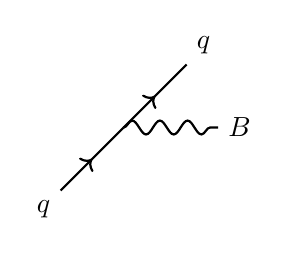
\begin{tikzpicture}[scale=0.8]
\begin{scope}[thick,decoration={
    markings,
    mark=at position 0.5 with {\arrow{>}}}
    ] 
\draw[postaction = {decorate}] (-1,-1) node[below left]{$q$} -- (0,0);
\draw[postaction = {decorate}] (0,0) -- (1,1) node[above right]{$q$};
\end{scope}

\draw[thick, snake it] (0,0) -- (1.5,0) node[right]{$B$};
\end{tikzpicture}}
\qquad
 \subfigure[]{
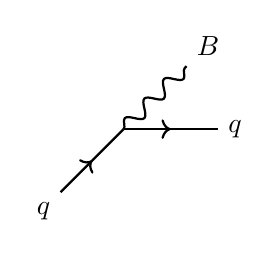
\begin{tikzpicture}[scale=0.8]
\begin{scope}[thick,decoration={
    markings,
    mark=at position 0.5 with {\arrow{>}}}
    ] 
\draw[postaction = {decorate}] (-1,-1) node[below left]{$q$} -- (0,0);
\draw[postaction = {decorate}] (0,0) -- (1.5,0) node[right]{$q$};
\end{scope}

\draw[thick, snake it] (0,0) -- (1,1) node[above right]{$B$};
\end{tikzpicture}}
\qquad
 \subfigure[]{
\begin{tikzpicture}[scale=0.8]
\begin{scope}[thick,decoration={
    markings,
    mark=at position 0.5 with {\arrow{>}}}
    ] 
\draw[postaction = {decorate}] (1,1)  node[above right]{$\bar{q}$}-- (0,0) ;
\draw[postaction = {decorate}] (0,0)  -- (1.5,0) node[right]{$q$};
\end{scope}

\draw[thick, snake it] (-1,-1) node[below left]{$B$} -- (0,0) ;
\end{tikzpicture}}
\qquad
 \subfigure[]{
\begin{tikzpicture}[scale=0.8]
\draw[thick, snake it] (-1,-1) node[below left]{$B$} -- (1,1) node[above right]{$B$};
\end{tikzpicture}}
\caption{The diagrams involving dark photons which contribute to splitting functions. (a), (b), (c), (d) show the contributions to $P_{qq}^{(0,0,1)}(x)$, $P_{Bq}^{(0,0,1)}(x)$, $P_{qB}^{(0,0,1)}(x)$ and $P_{BB}^{(0,0,1)}(x)$, respectively (note at this order, $P_{BB}^{(0,0,1)}(x)$ is proportional to a delta function, $\delta(1-x)$, indicating the lack of possible splitting in this channel).}
\label{fig:splittingfunctions}
\end{figure}

%
The coefficients $P_{ij}^{(0,0,1)}$ can be calculated directly by
finding the most collinearly-divergent parts of the four dark
splitting channels pictured in Fig.~\ref{fig:splittingfunctions}. The only non-zero contributions are given by $ij=qq, qB, Bq$ and $BB$ (the results are the same for antiquarks).
A summary of the calculation is given in App. A of Ref.~\cite{McCullough:2022hzr}; 
however, a detailed calculation is not strictly necessary, since the form
of the interaction Lagrangian Eq.~(\ref{eq:dm_lagrangian}) is identical
to that of the electromagnetic-hadronic interaction in the SM,
except with a universal coupling $\frac{1}{3}g_B$ to all quarks and antiquarks.
It follows that the splitting function contributions provided by the
dark photon $B$ will be identical (up to a factor of $\frac{1}{9}$, due to
our convention for the universal coupling) to those provided by the
photon $\gamma$; in particular, we can quote the required leading-order
splitting functions by comparing to \cite{Bertone:2015lqa}:
\begin{align}
\label{eq:splittingfunctions}
P_{qq}^{(0,0,1)}(x) &= \frac{1}{9}P_{qq}^{(0,1,0)}(x) = \frac{1+x^2}{9(1-x)_+} + \frac{1}{6} \delta(1-x), \notag\\\notag\\
 P_{BB}^{(0,0,1)}(x) &= \frac{1}{9} P_{\gamma\gamma}^{(0,1,0)}(x)= -\frac{2}{27}\delta(1-x), \notag\\ \\
P_{qB}^{(0,0,1)}(x) &= \frac{1}{9} P_{q\gamma}^{(0,1,0)}(x) = \frac{x^2 + (1-x)^2}{9},\notag\\\notag\\
 P_{Bq}^{(0,0,1)}(x) &= \frac{1}{9} P_{\gamma q}^{(0,1,0)}(x) = \frac{1}{9} \left( \frac{1 + (1-x)^2}{x} \right). \notag
\end{align}
%To solve the modified DGLAP equations~\eqref{eq:basicdglap}, we must
%also specify initial conditions for the dark photon at the initial scale $Q_0 = 1.65\ \text{GeV}$. 
%Given that we consider masses $m_B \in [2,80]$ GeV, we set $B(x,Q^2)
%= 0$ for all $Q < m_B$, and we generate the dark photon PDF dynamically
%at the threshold $Q = m_B$ from PDF evolution, similar to the
%treatment of heavy quarks in the ZM-VFN scheme~\cite{Maltoni:2012pa,Bertone:2017djs}, and the tau
%PDF in~\cite{Bertone:2015lqa}. Hence the dark photon PDF is always
%proportional to the dark photon coupling $\alpha_B$ and to
%$\log(Q^2/m_B^2)$ for $Q>m_B$. 

\subsection{PDF sets with dark photons}

We have implemented the modified DGLAP equations described in~Sec. \ref{subsec:dglap} in the
public APFEL PDF evolution code~\cite{Bertone:2013vaa}, which is an accurate and flexible that can be used to perform PDF evolution up to NNLO
in QCD and NLO in QED, using a variety of heavy flavour schemes.
The evolution is performed in $x$-space,\footnote{Rather than Mellin $N$-space, which is an alternative obtained by taking the Mellin transform of the DGLAP equations.} and uses a rotated 
basis of PDFs such that a maximal number of PDF flavour combinations
evolve independently. If we define the following vector of PDFs:
\begin{equation}
\label{eq:singlet}
\vec{q}^S = \begin{pmatrix} g \\ \gamma \\ \Sigma \\ \Delta_{\Sigma} \\ B\end{pmatrix},
\end{equation}
where:
\begin{equation}
\label{eq:singlet2}
\Sigma = \sum_{f=u,d,s,c} (f + \bar{f}), \qquad \Delta_{\Sigma} = \sum_{f=u,c} (f + \bar{f}) - \sum_{f=d,s} (f + \bar{f}),
\end{equation}
then we can choose further independent flavour combinations of PDFs, spanning the
complete space of PDFs, such that all of the remaining flavour combinations' evolution equations decouple;
 this greatly simplifies the computational work. The remaining matrix equation for $\vec{q}^S$ can 
 be shown to take the form:
 \renewcommand{\arraystretch}{0.8}
\begin{equation}
\label{eq:dglapevolution}
\mu_F^2 \frac{\partial \vec{q}^S}{\partial \mu_F^2} = \left(\begin{array}{cccc|c} & & & &  0 \\ & \ddots& \ddots& & 0 \\ & \ddots& \ddots& & P_{q B} \\[1ex] & & & & P_{q B} \\[1ex] \hline 0 & 0 & P_{Bq} & 0 & P_{BB} \end{array}\right) \otimes \vec{q}^S.
\end{equation}
Here, the dots denote the relevant SM matrix, with the quark-quark splitting function corrected with a dark contribution as appropriate. This equation (together with the other decoupled scalar equations) is solved using an adaptive step-size fifth-order Runge-Kutta method, 
as described in~\cite{Bertone:2013vaa}.% and [...].

To solve the modified DGLAP equations~\eqref{eq:basicdglap}, we must
also specify initial conditions for the dark photon;
this is where we make appropriate ans\"{a}tze for the functional form of the dark photon at the initial scale $Q_0 = 1.65\ \text{GeV}$. 
If the mass of the dark photon $m_B$ were less than the scale $Q_0$, we
could postulate a functional form for the initial dark photon PDF
assuming that the dark photon PDF is primarily generated by quark
splitting.
An appropriate initial condition in this case would be given by:
\begin{equation}
\label{eq:lowmassansatz}
B(x,Q_0^2) = \frac{\alpha_B}{2\pi} \log\left( \frac{Q_0^2}{m_B^2} \right) \sum_{j=1}^{n_f} (P_{Bq_j} \otimes (q_j(x,Q_0^2)+ \bar{q}_j(x,Q_0^2)),.
\end{equation}
On the other hand, we shall shortly describe that the region of interest in our case is $m_B \in [2,80]$ GeV;
in this region, we always have $m_B >
2$ GeV. Thus in our case, we always have $m_B > Q_0$; that is, the mass threshold is always greater than
the initial scale. As a result, we set $B(x,Q^2) = 0$ for all $Q < m_B$ and we generate the dark photon PDF dynamically at the threshold $Q = m_B$ from PDF evolution, similar to the treatment of heavy quarks~\cite{Maltoni:2012pa,Bertone:2017djs}, and the tau PDF in~\cite{Bertone:2015lqa}. 



Using the modified code, we produce a PDF set and a corresponding LHAPDF
grid~\cite{Buckley:2014ana} including dark photons, for each given
value of the dark photon mass and coupling that we consider. 
We focus on the introduction of a dark photon into the evolution of the
{\tt NNPDF3.1luxQED} set~\cite{Bertone:2017bme},\footnote{This
    set will be soon superseded by the PDF set including QED effects
    obtained starting from NNPDF4.0~\cite{NNPDF:2021njg}.} which provides our
SM baseline, namely an NNLO
global PDF analysis of all standard parton flavours together with a photon PDF (the photon
PDF in this set is determined using the state-of-the-art {\tt LUXqed}
method~\cite{Manohar:2017eqh}).\\

\noindent For demonstration purposes, we now proceed to display the key
results from a `dark PDF set' in a particular scenario
that is permitted according to the bounds given in
Ref.~\cite{Ilten:2018crw}, namely:
%two scenarios (both of which are permitted according to the bounds given in~\cite{Ilten:2018crw}):
%\begin{itemize}
%\item \textbf{Scenario I.} The dark photon has mass $m_B = 5\ \text{GeV}$ and coupling $\alpha_B = 10^{-3}$.
%\item \textbf{Scenario II.} The dark photon has mass $m_B = 50\ \text{GeV}$ and coupling $\alpha_B = 3 \times 10^{-3}$.
%\end{itemize}
\begin{equation}
  \label{eq:value}
  m_B = 50\,\, \text{GeV}, \qquad \alpha_B = 3 \times 10^{-3},
\end{equation}
which corresponds to taking $g_B = 1.94 \times 10^{-1}$. As described
above, a massless dark photon is generated dynamically at the threshold $Q = m_B$, and is set
to zero before this threshold is reached. We have chosen a sufficiently
high (admissible) value of the coupling to display the impact
upon PDFs and parton luminosities. 
%
\begin{figure}[hbt]
\centering
\includegraphics[width=0.49\textwidth]{darkphoton_figures/vhigh_dark_photon_comparison_100GeV.pdf}
\includegraphics[width=0.49\textwidth]{darkphoton_figures/vhigh_dark_photon_comparison_1TeV.pdf}
\caption{Comparison of $x\gamma(x,Q^2)$ and $xB(x,Q^2)$ at $Q=100\ \text{GeV}$ (left) and $Q=1\ \text{TeV}$ (right)
for the values of dark photon mass and coupling given in
Eq.~\eqref{eq:value}. The percentage relative 68\% C.L. PDF
uncertainties of the photon and the dark photon are
  displayed in the bottom inset.}
  %The dark photon uncertainty is mostly comparable to the photon uncertainty... \JM{perhaps add more comments here?}}
\label{fig:dark_pdfs}
\end{figure}

In Fig.~\ref{fig:dark_pdfs}, we display both the photon and dark
photon PDFs in our representative dark set (obtained by setting the
dark photon coupling and mass at the values given in
Eq.~\eqref{eq:value}) at the scales $Q = 100\ \text{GeV}$ and $Q=1\ \text{TeV}$,
and show their relative PDF uncertainties. As anticipated, the dark photon PDF features 
the same functional form as the photon PDF (this is to be expected
since the photon and dark photon splitting functions are identical up
to scaling), but its density is smaller since $\alpha_B \lesssim
\alpha$. Furthermore, it can be shown that increasing $\alpha_B$, and also moderately decreasing 
$m_B$, increases the similarity of the dark photon and photon PDFs.
The dark photon uncertainty is mostly comparable to the photon
uncertainty up to $x\sim 0.4$, and then increases faster than the photon
uncertainty. This is due to the dark photon being generated off the
singlet PDF (the sum of all quarks and antiquarks) at its mass
threshold with a rather small coupling; in particular, the dark
photon uncertainty is comparable to the uncertainty of the singlet PDF
scaled by a factor of  $\alpha_B$. This makes it comparable to the
photon PDF uncertainty (for the choice of $\alpha_B$ and $m_B$ of
Eq.~\eqref{eq:value}), except in the large-$x$ region where the singlet PDF uncertainty dramatically increases,
resulting in the dark photon PDF uncertainty to consistently increase up to $\sim10\%$ at
$x\sim 0.6$. We have verified that for larger couplings the
uncertainty increases, as one would expect. 


Now that we have introduced a new parton in the proton, it is 
interesting to ask how much `space' it takes up; this can be quantified
by determining the momentum carried by the dark photon at 
different energy scales. By definition, the momentum fraction carried by any given
parton flavour $f$ at the scale $Q$ is given by:
\begin{equation}
\label{eq:momfraction}
\langle x\rangle_f(Q) := \int\limits_{0}^{1} dx\ xf(x,Q).
\end{equation}
In Table.~\ref{tab:dark_momentum}, we give a comparison between the
momentum carried by the dark photon, the photon and the singlet for
the representative dark PDF
set computed using the values specified in Eq.~\eqref{eq:value}, and
compare them to the baseline SM PDF set, at $Q=100$ GeV and $Q=1$ TeV. 
We observe that the fraction of the proton momentum carried by the
dark photon increases with the scale $Q$, which is to be expected 
by analogy with the photon's behaviour. Depending on the coupling
and the mass of the dark photon, the latter carries up to a fraction
of percent of the proton momentum's fraction at $Q\approx1\
\text{TeV}$. 
\begin{table}[tb]
\centering
\begin{tabularx}{\textwidth}{X|C{1.8cm}C{1.8cm}C{1.8cm}C{1.8cm}}
\toprule
$\langle x\rangle_f(Q=100$ GeV) & $f=\Sigma$ & $f=\gamma$ & $f=B$ \\
\midrule
Baseline &  50.23\% &  0.4241\% & 0\% \\
Dark set & 50.17\% & 0.4241\% &0.03214\%  \\
\midrule
$\langle x\rangle_f(Q=1$ TeV) & $f=\Sigma$ & $f=\gamma$ & $f=B$ \\
\midrule
Baseline &  48.36\% &  0.5279\% & 0\% \\
Dark set & 48.12\% &  0.5275\% & 0.1357\%  \\
\bottomrule
\end{tabularx}
%\includegraphics[width=0.7\textwidth]{vhigh_momentum_distribution_log.pdf}
\caption{A comparison between the momentum fraction percentage carried by the
  singlet $\Sigma$, the photon $\gamma$, and the dark photon $B$ at $Q=100$ GeV and $Q=1$ TeV,
  for the baseline SM set and the dark
  PDF set, obtained with the photon coupling and mass given in Eq.~\eqref{eq:value}. The momentum
fraction is computed on the central replica in each case. }
\label{tab:dark_momentum}
\end{table}


Crucially, the presence of a dark photon in the DGLAP equations also
modifies the evolution of all other flavours of PDFs due to the
coupling of the PDFs via the modified DGLAP equations
Eq.~(\ref{eq:basicdglap}).
We expect that the modification of the quark and antiquark 
flavours is strongest, as the dark photon is directly coupled to
them. We also anticipate a modification to the gluon and photon
PDFs, but these will be second order effects, so we expect that they
will be smaller in comparison. Moreover, the density of each of the
flavours should reduce, as the new dark photon `takes up space' in the
proton which was previously occupied by the quark flavours.
\begin{figure}[tb]
\centering
\includegraphics[width=0.49\textwidth]{darkphoton_figures/singlet_ratios_1TeV.pdf}
\includegraphics[width=0.49\textwidth]{darkphoton_figures/uvalence_ratios_1TeV.pdf}
\caption{In solid orange, the ratio between the central singlet PDF $\Sigma$ (left) and central $u$-valence
  PDF (right), drawn from the dark benchmark scenario in Eq.~\eqref{eq:value}, 
  to the baseline SM central replica at $Q = 1\
  \text{TeV}$. In dashed orange, the same ratios but between the SM baseline and a dark PDF set
  produced using $m_B = 50\ \text{GeV}, \alpha_B = 5 \times 10^{-3}$. In each case, the uncertainty bands
  represent the 68\% C.L. PDF uncertainties of the baseline set (in blue) 
  and the projected PDF uncertainties at the HL-LHC, determined
  from Ref.~\cite{Khalek:2018} (in light blue). The deviation when $\alpha_B = 5 \times 10^{-3}$ approaches
  the boundary of the projected HL-LHC uncertainty bands, consistent with the behaviour we see in Fig.~\ref{fig:14tevlumis} later; increasing $\alpha_B$ (and also to a milder extent, decreasing $m_B$) pushes the deviation outside of projected HL-LHC uncertainty bands.
  See the main text for more details.}
\label{fig:ratio_quarks}
\end{figure}
Results are shown in Fig.~\ref{fig:ratio_quarks}, in which the ratio
between the central value of the dark-photon modified singlet
($u$-valence) PDF and the central value of the baseline singlet
($u$-valence) PDF are displayed and compared to the current 68\% C.L. PDF
uncertainty. 

We observe
that the modification of the singlet becomes visible at about $x\sim 0.2$ and
reaches 3\% at larger values of $x\sim 0.5$. This is well within the
68\% C.L. uncertainty of the singlet PDF from the baseline {\tt
  NNPDF3.1luxQED} NNLO set. However, thanks to the inclusion of a vast
number of new datasets and the increased precision of the methodology
used in global PDF analysis, the recent {\tt NNPDF4.0} NNLO
set~\cite{NNPDF:2021njg} 
displays significantly smaller large-$x$ uncertainty. Such a
decrease in PDF uncertainties goes in the direction indicated by the
dedicated study on how PDF
uncertainties will decrease in future, thanks to the inclusion of precise
HL-LHC measurements~\cite{Khalek:2018}. In particular, to give an indication
of how the modification of PDFs due to the presence of a dark photon might
come into tension with decreasing PDF uncertainties during the HL-LHC phase, 
we display the projected 68\% PDF uncertainties at
the HL-LHC determined in the `optimistic' scenario, Scenario 3, of Ref.~\cite{Khalek:2018}.
In this case, should PDF uncertainties decrease to the
level predicted by Ref.~\cite{Khalek:2018}, the distorted singlet PDF approaches the edge of the
projected PDF uncertainty at $x\sim \,0.1-0.3$ region, for the values given
in Eq.~\eqref{eq:value}. This is particularly relevant for the
analysis that we present in the next section. 




\newpage
\section{Phenomenological implications and projected bounds}
\label{sec:dark_pheno}

In this section we review the existing constraints on the dark photon.
Subsequently, in order to assess the impact of a non-zero dark photon
parton density on physical observables, we plot the parton luminosities
when the dark photon is included, as compared to our baseline SM set. 
We compare the predicted deviations with the current PDF
uncertainties and with the projected PDF uncertainties at the HL-LHC.
Finally, we motivate and present an analysis of projected HL-LHC Drell-Yan data 
and compare the maximal sensitivity we can achieve to the existing
bounds derived in the literature.

\subsection{Review of existing constraints on the dark photon}
\label{sec:existingconstraints}
To appreciate the utility of the dark photon PDF at colliders, we may compare to alternative probes.  Recent works considering this class of baryonic dark photon models include \cite{Dobrescu:2014fca,Dror:2017ehi,Ismail:2017fgq,Dror:2018wfl,Ilten:2018crw,Dobrescu:2021vak}.  There are a variety of competing constraints on this scenario, of varying theoretical robustness.

One class of constraints, first considered in detail in
\cite{Dobrescu:2014fca}, is theoretical and concerns the mixed $\text{U}(1)_B-$EW anomalies.  Suppose we envisage that the UV-completion of the model Eq.~\eqref{eq:value} is perturbative with $\text{U}(1)_B$ linearly realised.  In that case, the mixed anomaly must be UV-completed by some fermions with electroweak charges.  Early studies of the classes of fermions that can achieve this include \cite{Duerr:2013dza,FileviezPerez:2014lnj}.\footnote{Note also that the required fermions could serve as potential dark matter candidates, as discussed in \cite{FileviezPerez:2019jju,Perez:2020jyg,Perez:2021rbo}.}   In this perturbative UV-completion they will obtain their mass from spontaneous $\text{U}(1)_B$-breaking.  As a result, they will be coupled to the longitudinal mode of $B$ and an additional Higgs-like scalar with a Yukawa coupling $\lambda \propto M_F/v_B$, where $M_F$ is the fermion mass, $v_B$ is the $\text{U}(1)_B$-breaking expectation value, and we have assumed three sets of fermions with the same charge ($1/3$) as the left-handed fermions, for simplicity.  On the other hand we have $g_B  \propto M_B/v_B$ following from the charge and symmetry-breaking vacuum expectation value.  As a result, we expect:
\begin{equation}
g_B \approx \frac{2 \lambda}{3} \frac{M_B}{M_F} ~~,
\end{equation}
where the precise numerical factors are taken from \cite{Dobrescu:2014fca}.  Thus, requiring perturbativity $\lambda \lesssim 4 \pi$ implies an upper bound on $g_B$, where the factor $1/3$ follows from the fact that each family of fermions is in triplicate to mirror the QCD multiplicity of the SM quarks.  This limit is shown as a dashed line in Fig.~\ref{fig:limits} where we have taken $M_F\geq 90$ GeV for the electroweak-charged fermions. 

However, a number of implicit assumptions have been made which can weaken upon further inspection.  To see this, consider cancelling the anomaly with $N$ copies of the above class of fermions.  In this case the limit becomes:
\begin{equation}
g_B \lesssim \frac{8 \pi}{3} \frac{N}{3} \frac{M_B}{M_F} ~~.
\end{equation}
Hence we see that this theoretical limit makes not only the assumption of a weakly-coupled UV-completion, but also depends on assumptions of minimality of the UV completion as well.  As a result, while this limit does guide the eye as to the nature of the UV-completion, it cannot be considered a strong theoretical limit on the model parameters.

Another constraint which is very relevant in some UV-completions concerns Higgs boson decays.  In some UV-completions the radial mode of spontaneous symmetry breaking may mix with the Higgs boson, giving rise to Higgs decays to $B$'s.  Depending on the magnitude of the mixing angle the corresponding constraints can be strong, as demonstrated in \cite{Perez:2020izb}.  Care must be taken to consider these processes in any specific UV-completion, however as the rates depend strongly on the details of the UV-completion we do not include them in our analysis here, which is focussed on the irreducible model-independent IR physics.

The only truly model-independent theoretical limit comes from considering the scale at which the validity of the IR theory itself breaks down.  Given that the quark interactions are vector-like there is no possibility of tree-level unitarity violation in quark scattering mediated by $B$, thus we must look to quantum effects.  In this case the mixed-anomaly becomes relevant and renders the theory non-unitary unless \cite{Preskill:1990fr}:
\begin{equation}
g_B \lesssim \frac{(4 \pi)^2}{3 \alpha_W} \frac{M_B}{M_\Lambda} ~~,
\end{equation}
where $\alpha_W$ is the $\text{SU}(2)$ fine structure constant at the electroweak scale and $M_\Lambda $ is the energy scale at which the theory becomes strongly coupled.  Numerically this is
\begin{equation}
g_B \lesssim \frac{3M_B}{5 \text{ GeV}} \frac{10 \text{ TeV}}{M_\Lambda} ~~,
\end{equation}
which is too weak to be relevant for our purposes.  As a result we conclude that the effective theory considered here is valid throughout the energy scales under investigation. However, we note that, as shown in
\cite{Dobrescu:2021vak}, the mixing with the $Z$-boson is sensitive to
the details of the UV-completion; for this reason we restrict the mass range under
investigation to $m_B \leq 80\ \text{GeV}$, above which these UV-dependent effects can be important.  %One could impose \ae sthetic constraints on the UV completion in order to constrain the parameters of the IR theory, however in this case the model-dependence of the constraint must be kept in mind.

There are three relevant classes of experimental constraints.  The first
concerns the exotic $Z$-boson decays $Z\to B\gamma$.  These constraints
were calculated in \cite{Dror:2017ehi} based on the LEP analysis for
$Z\to H\gamma$, $H\to$hadrons~\cite{L3:1996dmt}.\footnote{Note that
  this reference does not appear in~\cite{Dror:2017ehi}, but instead
  in~\cite{L3:1991kow,L3:1992kcg}, however the authors of
  \cite{Dror:2017ehi} have confirmed that the limits follow from a
  recasting of \cite{L3:1996dmt}.} This limit, relevant to the higher
mass range, is shown in red in Fig.~\ref{fig:limits}.  The second
class of constraints at lower masses concerns exotic $\Upsilon$ decays
\cite{Carone:1994aa,Aranda:1998fr}, where the constraint is dominated
by limits on $\Upsilon(1S)\to 2$ jets \cite{ARGUS:1986nzm}, shown in
blue in Fig.~\ref{fig:limits}. Finally, there are additional searches for
hadronically decaying resonances at hadron colliders
\cite{Dobrescu:2013cmh,Shimmin:2016vlc,ATLAS:2019itm,Dobrescu:2021vak}.
The strongest are from CMS $B+$ISR searches
\cite{CMS:2019xai,CMS:2019emo}, shown in yellow in
Fig.~\ref{fig:limits}. 

\subsection{Effects of the dark photon on parton luminosities}
In Sec.~\ref{sec:dglap}, we showed that the presence of a dark photon modifies
all other flavours of PDFs via the mixing associated with the
DGLAP evolution equations, with a modification that is proportional to
$\alpha_B$ and the logarithm of $m_B$. 
In order to assess the impact of a dark photon
parton density on physical observables, and thus extract the 
sensitivity that the LHC can achieve on the
parameters of the model, in the following subsection
we compare the size of the dark parton luminosities to luminosities
involving the other partons, and assess the impact of the dark photon
on the dominant partonic channels.

%Given that in the computation of the cross sections of hadron-collider processes, PDF contributions
%factorise in the form of, it
%is useful to study the behaviour of the parton luminosities of the different initial states, by
%including also the dark photon. %{\color{red} Text here very similar to lepton PDF paper.}
Parton luminosities are doubly differential quantities defined as:
\begin{equation}
\frac{d{\cal L}_{ij}}{dyd\tau}=f_i(x_1,Q)f_j(x_2,Q)\qquad x_{1,2}=\sqrt{\tau}\exp(\pm
y)\qquad \tau=\frac{M_X^2}{S},
\end{equation}
where $S$ is the squared centre-of-mass energy of the hadronic collision, $M_X$ is the invariant mass
of the partonic final state, $y$ is the rapidity of the partonic final state, and 
$f_i(x,Q)$ is the PDF of the $i^{\rm th}$ parton evaluated at the
scale $Q$. Different choices for $Q$ can be adopted in order to improve predictions
of a particular process and/or distribution.
At the level of pure luminosities, without the convolution with
any specific matrix element, the factorisation scale can be naturally
set to $Q = M_X$. For plotting purposes, it is useful to define the
$M_X$-differential luminosities, given by:
\begin{equation}
  \label{eq:lumidef}
\Phi_{ij}(M_X) \,=\,\frac{d{\cal L}_{ij}}{dM_X^2}=\frac{1}{S}\,\int\limits_{M_X^2/S}^1
\frac{dx}{x}\ f_i(x,M_X)f_j\left(\frac{M_X^2}{xS},M_X\right).
\end{equation}

%
\begin{figure}[tb]
\centering
% \subfigure[]{
% \includegraphics[scale=0.43]{high_BB_gmgm_luminosity_14TeV.pdf}}
% \quad
%  \subfigure[]{
\includegraphics[width=0.7\textwidth]{darkphoton_figures/vhigh_BB_gmgm_luminosity_14TeV.pdf}
\caption{Comparison of the absolute value of the $\Phi_{BB}$,
  $\Phi_{qB}$ central luminosities and the $\Phi_{\gamma\gamma}$  and
  $\Phi_{qq}$ central luminosities as a function of the invariant mass $M_X$
  at the centre of mass energy $\sqrt{s} = 14\ \text{TeV}$ for the dark PDF set obtained with 
 the dark photon coupling and mass set in Eq.~\eqref{eq:value}.% , in
  % Scenario I and II respectively. Note that in Scenario II, the gradient of
  % $\Phi_{BB}$ and $\Phi_{Bq}$ plateaus as we approach $M_X = 100\ \text{GeV}$ from 
  % above; this is to be expected, since these luminosities vanish for $M_X \leq 50\ \text{GeV}$,
  % and numerical instability increases in their computation as we approach this mass threshold.
}
\label{fig:lowdarkmass}
\end{figure}
%
We first compare the size and the $M_X$-dependence of the different
parton luminosities in the candidate dark PDF set obtained by setting the mass and the coupling to the
values indicated in Eq.~\eqref{eq:value}. In Fig.~\ref{fig:lowdarkmass} we plot $\Phi_{BB},
\Phi_{Bq}$ as compared to $\Phi_{q\bar{q}}$,
$\Phi_{\gamma\gamma}$. We
observe that, while the $BB$ channel is suppressed by two powers of
the dark coupling, and its size never exceeds more than a fraction of a percent of the
$q\bar{q}$ luminosity, the $Bq$ channel grows from about 2\% of the
$q\bar{q}$ luminosity at $M_X\sim$ 1 TeV to about 8\% of the
$q\bar{q}$ luminosity at larger values of the invariant mass. Its
contribution exceeds that of $\gamma\gamma$ scattering by one order of magnitude. 

\begin{figure}[bht]
\centering
% \subfigure[]{
% \includegraphics[scale=0.43]{high_uubar_luminosity_14TeV.pdf}}
% \quad
%  \subfigure[]{
% \includegraphics[scale=0.43]{vhigh_uubar_luminosity_14TeV.pdf}}
% %
 \subfigure[$m_B=50\ \text{GeV}, \alpha_B = 3 \times 10^{-3}$]{
\includegraphics[scale=0.43]{darkphoton_figures/vhigh_qqbar_luminosity_14TeV.pdf}
}
\quad
 \subfigure[$m_B=50\ \text{GeV}, \alpha_B = 5 \times 10^{-3}$]{
\includegraphics[scale=0.43]{darkphoton_figures/mB_50_alphaB_5e-3_qqbar_luminosity_14TeV.pdf}
}
\quad
  \subfigure[$m_B=5\ \text{GeV}, \alpha_B = 3 \times 10^{-3}$]{
 \includegraphics[scale=0.43]{darkphoton_figures/mB_5_alphaB_3e-3_qqbar_luminosity_14TeV.pdf}}
 \quad
  \subfigure[$m_B=5\ \text{GeV}, \alpha_B = 5 \times 10^{-3}$]{
 \includegraphics[scale=0.43]{darkphoton_figures/mB_5_alphaB_5e-3_qqbar_luminosity_14TeV.pdf}}
 %
\caption{The ratio $\Phi_{q\bar{q}}^{\text{Dark}}/\Phi_{q\bar{q}}^{\text{SM}}$ for
  % each of the quark flavours $q = u, d$ and
  the total quark-anti-quark luminosity, at the centre of mass energy
  $\sqrt{S} = 14\ \text{TeV}$ for the values of mass and coupling
  indicated under each panel. 
  In each panel, the dark blue bands correspond to the current PDF
  uncertainty, while the light blue bands show the expected uncertainty on the
  PDF luminosity at the HL-LHC. See main text for more details.}
\label{fig:14tevlumis}
\end{figure}
%
We now turn to assess the change in the other luminosities, as a result of the
inclusion of a non-zero dark photon parton density.
In Fig.~\ref{fig:14tevlumis} we display the ratio of the dark-photon
modified quark-antiquark integrated luminosity
$\Phi_{q\bar{q}}^{\text{Dark}}$ with the baseline one, $\Phi_{q\bar{q}}^{\text{SM}}$ at the centre of mass energy
  $\sqrt{S} = 14\ \text{TeV}$, for different values of the $\alpha_B$
  and $m_B$ parameters, starting from our benchmark values, Eq.~\eqref{eq:value}.
  In each figure, the dark blue band corresponds the 68\% C.L. PDF
  uncertainty of the NNLO baseline {\tt NNPDF3.1luxQED} set, while the
  green bands show the projected PDF uncertainty on the
  parton luminosity at the HL-LHC; this estimate for the uncertainty
  on the PDF luminosity is obtained from the `optimistic' scenario, Scenario 3,
  analysed in \cite{Khalek:2018}, as above. 
  %
%  To compute the projected reduction in the
%  PDF uncertainty at the HL-LHC, we take the ratio of the 68\% C.L. 
%  relative uncertainties of the luminosity computed using the public {\tt
%    PDF4LHC15\_nnlo\_hllhc\_scen3}  PDF set associated with the
%  optimistic scenario released alongside
%  Ref.~\cite{Khalek:2018} and those computed with the reference set in
%  the projection study, namely the {\tt PDF4LHC15} PDF
%  set~\cite{Butterworth:2015oua}. We then multiply the 68\% C.L. PDF
%  uncertainty of the NNLO baseline by the ratio to obtain the
%  projected PDF uncertainty at the LHC. 
  Starting from the values of Eq.~\eqref{eq:value}, we observe that
  the deviation in the $q\bar{q}$ luminosity due to the presence of
  the dark photon is significant compared to the size of the
  projected PDF uncertainties at the HL-LHC. Decreasing the mass of
  the dark photon by a factor of 10 increases the impact of the dark
  photon on $q\bar{q}$ initiated observables, while increasing the
  coupling by less than a factor of 2 brings the luminosity beyond the
  edge of the 68\% C.L. error bands. %The appreciable deviation between
 % the dark luminosity and the projected uncertainties on the baseline
  %SM luminosities encourage the phenomenological study in the sequel.

Crucially, the effect of the dark photon is much larger in the $q\bar{q}$-initiated processes than in
any of the other channels, including $qq$, $qg$ and $gg$. This motivates the study of the high-mass Drell-Yan tails that we put
forward in the following section. 


\subsection{Constraints from precise measurements
  of high-energy Drell-Yan tails}

Given that the $q\bar{q}$ channel is the most affected by the presence of a non-zero dark photon parton density, in this
study we focus on precise measurements of the high-mass Drell-Yan
tails at the HL-LHC. It is important to note that these projected data are not
included in the fit of the input PDF set used as a baseline,
otherwise, as was explicitly shown in ~\cite{Carrazza:2019sec,greljo_parton_2021,Iranipour:2022iak}, the interplay between the fit of the
new physics parameters and the fit of the PDF parametrisation at the
initial scale might distort the results. 

To generate the HL-LHC pseudodata for neutral-current
high-mass Drell-Yan cross sections at $\sqrt{S}=14$ TeV, we follow the procedure of~\cite{greljo_parton_2021}.
Namely, we adopt as reference the CMS  measurement at 13 TeV~\cite{CMS:2018mdl} based on $\mathcal{L}=2.8$ fb$^{-1}$.
%
The dilepton invariant mass distribution $m_{\ell\ell}$ is evaluated using the same selection
and acceptance cuts of~\cite{CMS:2018mdl}, but now with an extended
binning in $m_{\ell\ell}$ to account for the increase in luminosity.
%
We assume equal cuts for electrons and muons, and impose $|\eta_\ell|\le 2.4$,
$p_T^{\rm lead}\ge 20$ GeV, and $p_T^{\rm sublead}\ge 15$ GeV for the two
leading charged leptons of the event.
We restrict ourselves to  events with $m_{\ell\ell}$ greater than $500$ GeV, so that 
the total experimental uncertainty is not limited by our modelling
of the expected systematic errors, by making our projections unreliable.
%
To choose the binning, we require that the expected number of events per bin
is bigger than 30 to ensure the applicability of Gaussian statistics.
%
Taking into account these considerations, our choice of binning
for the $m_{\ell\ell}$ distributions at the HL-LHC both in the muon and electron channels 
are displayed in Fig.~\ref{fig:data-theory} with the highest energy bins reaching $m_{\ell\ell}\simeq 4 $ TeV.
In total, we have two invariant mass distributions of 12 bins each, one in the electron and one in the muon channels.

Concerning uncertainties, in ~\cite{greljo_parton_2021} this data is produced by assuming that the HL-LHC phase will
operate with a total integrated luminosity of $\mathcal{L} = 6\ \text{ab}^{-1}$
(from the combination of ATLAS and CMS, which provide ${\cal L}=3 \,{\rm ab}^{-1}$ each),
and also assuming a five-fold reduction in systematic uncertainty
compared to ~\cite{CMS:2018mdl}. 
We regard this scenario as {\it optimistic} in this paper; we also
manipulated the projected data so that it reflected a more {\it
  conservative} possibility, where the total integrated luminosity of
the high-mass Drell-Yan tail measurements is $\mathcal{L} = 3\
\text{ab}^{-1}$ (say, for example, they are made available only by
either ATLAS or CMS) and with a two-fold (rather than a five-fold) reduction in systematic uncertainties.

For these projections, the reference theory is the SM, with
theoretical predictions evaluated at NNLO in QCD including full 
NLO EW corrections (including in particular the photon-initiated
contributions); note, however, that the Drell-Yan production has been recently computed at
N${}^3$LO in QCD~\cite{Duhr:2020seh,Duhr:2021vwj}. In the kinematical
region that is explored by our HL-LHC projections ($m_{\ell\ell}>500$
GeV), the perturbative convergence of the series is good and
the N${}^3$LO computation is included within the NNLO prediction, with
missing higher order uncertainty going from about 1\% to a fraction of
a percent. Given the good perturbative convergence of
the matrix element calculation, and the absence of N${}^3$LO PDFs that match
the accuracy of the N${}^3$LO computation of the matrix element, we use the NNLO QCD and NLO EW accuracy of our calculations, both for the SM
baseline and for the dark-photon modified PDF set that we use to
compute the maximal sensitivity to the dark photon parameters. 

The central PDF set used as an input to generate the theoretical prediction is the SM baseline
that we use throughout the paper, namely the NNLO {\tt NNPDF3.1luxQED} set.
The central values for the HL-LHC pseudodata are then generated
by fluctuating the reference theory prediction by the expected total experimental
uncertainty, namely
\begin{equation}
  \label{eq:hllhc}
\sigma^{\rm hllhc}_{i} \equiv \sigma^{\rm th}_{i} \left( 1+ \lambda
  \delta_{\cal L}^{\rm exp} +  r_i\delta_{{\rm tot},i}^{\rm exp}   \right) \, , \qquad i=1,\ldots,n_{\rm bin} \, ,
\end{equation}
where $\lambda,r_i$ are univariate Gaussian random numbers, $\delta_{{\rm tot},i}^{\rm exp}$
is the total (relative) experimental uncertainty corresponding to this
specific bin
(excluding the luminosity and normalisation uncertainties), and $\delta_{\cal L}^{\rm exp}$
is the luminosity uncertainty, which is fully correlated amongst all
the pseudodata bins of the same experiment. We take this luminosity uncertainty to be
$\delta_{\cal L}^{\rm exp}=1.5$\%  for both ATLAS and CMS, as done in~\cite{Khalek:2018}.

To obtain bounds on the dark photon mass and coupling, we select a grid of benchmark
points $(m_B, \alpha_B)$ in the dark photon parameter space; our scan consists of $21$ points, distributed as a rectangular grid
with masses $m_B = 2, 5, 8, 10, 20, 50, 80\ \text{GeV}$ and couplings
$\alpha_B = 10^{-3}, 2\times10^{-3}, 3 \times 10^{-3}$. We then construct dark PDF sets at each 
of these benchmark points (thus a total of $21$ PDF sets, in each case including quarks, antiquarks, the gluon, the photon and the dark photon PDFs), using the 
appropriate values of $m_B, \alpha_B$, and hence
compute theoretical predictions in both the \textit{optimistic} and \textit{conservative} scenarios at each grid point. The predictions
are produced assuming that the primary contribution comes from the
$q\bar{q}$ channel; in particular, we note that the partonic diagrams that include a dark
photon in the initial state (such as $Bq\to \bar{q}l^+l^-$ or $B\bar{q}\to
ql^+l^-$) are suppressed by two powers of $\alpha_B$, one from the
dark photon PDF and one from the matrix element, and therefore are
suppressed beyond the accuracy of our calculation. 

\begin{figure}
\centering
\includegraphics[width=0.9\textwidth]{darkphoton_figures/data_theory_comparison.pdf}
\caption{\textbf{Top:} data-theory comparison between HL-LHC pseudodata in the electron channel generated according to
  Eq.~\eqref{eq:hllhc} (grey, with \textit{optimistic} uncertainties displayed), and the theoretical predictions obtained using
  the NNLO baseline PDF set {\tt NNPDF3.1luxQED} (blue) and
  those obtained using the dark PDF sets produced with parameters $(m_B,\alpha_B) = (5\ \text{GeV},3\times 10^{-3}), (5\ \text{GeV}, 5 \times 10^{-3})$ (yellow, green respectively).
\textbf{Middle:} ratio of the baseline SM central predictions obtained using the baseline, and the central predictions
  obtained using the two representative dark PDF sets, to the central values of the pseudodata.  The relative experimental
  uncertainties in both the {\it optimistic} scenario (dark grey) and
  {\it conservative} scenario (light grey) are displayed. \textbf{Bottom:} ratio of the central predictions obtained using the two
  representative dark PDF sets to the baseline SM central predictions, with both the PDF uncertainty from the baseline PDF set (dark blue) and the projected PDF uncertainty
  at the HL-LHC in the optimistic scenario of ~\cite{Khalek:2018}
  (light blue) displayed.
} 
\label{fig:data-theory}
\end{figure}
%
In Fig.~\ref{fig:data-theory} we display the data-theory comparison
between the HL-LHC pseudodata in the electron channel, generated according to
Eq.~\eqref{eq:hllhc}, and both the SM theoretical predictions obtained using
  the NNLO baseline PDF set {\tt NNPDF3.1luxQED} and the predictions
  obtained using the dark PDF sets produced with the dark photon mass
  and coupling set
  to $(m_B=5\,{\rm GeV},\alpha_B=3\times 10^{-3})$ 
  and $(m_B=5\,{\rm GeV},\alpha_B=5\times 10^{-3})$ respectively. We also display 
 the ratio between the central values of those predictions and the
 central values of the pseudodata as compared to their relative
 experimental uncertainty in both the
 {\it optimistic} and {\it conservative} scenarios.
We see that whilst the SM predictions are within the $1\sigma$
experimental uncertainty (by construction), the dark-photon modified
predictions display significant deviations. 
In the bottom inset we show the ratio between the predictions
obtained in the two representative dark photon scenarios to the
central SM theoretical predictions obtained with the
the baseline SM PDF set. PDF uncertainties are shown; we display
both the current PDF uncertainty of the NNLO baseline PDF set {\tt
  NNPDF3.1luxQED} and the projected PDF uncertainties 
  at the HL-LHC, obtained as described at the beginning of this
  section. Comparing the size of the PDF uncertainties to the size of the
  projected experimental uncertainties at the HL-LHC, we observe
  that whilst the current PDF uncertainties are comparable to the
  experimental uncertainties of the projected data, the projected
  HL-LHC uncertainties are subdominant as compared to the
  experimental uncertainties of the pseudodata.

The $\chi^2$-statistic of the resulting dark PDF set's predictions on high-luminosity high-mass neutral-current DY data is defined as: 
\begin{equation}
\label{eq:chi2stat}
\chi^2(m_B, \alpha_B) := ||\vec{T}(m_B, \alpha_B) - \vec{D}||^2_{\Sigma^{-1}},
\end{equation}
where $||\vec{v}||_{A}^2 = \vec{v}^T A \vec{v}$, $\vec{D}$ is the projected data, 
$\vec{T}(m_B,\alpha_B)$ are the theoretical predictions using a dark
PDF set containing a dark photon of mass $m_B$ and coupling
$\alpha_B$, and $\Sigma$ is the total
covariance matrix (incorporating both experimental and theoretical
uncertainties):
\begin{equation}
\Sigma = \Sigma^{\rm th}+\Sigma^{\rm exp}.
\end{equation}
From Fig.~\ref{fig:data-theory} we observe that, depending on the assumption we make on PDF
uncertainties in the HL-LHC era, it may be important to
include the PDF uncertainties in the theory covariance matrix, while
the component of the theory covariance matrix associated with the
scale uncertainty of the NNLO computation is subdominant. 
Of course, it would be unrealistic to assume that the PDF uncertainty will not decrease as compared to the
  uncertainty of the {\tt NNPDF3.1luxQED} baseline, given that we already know
  that in the updated {\tt NNPDF4.0} set~\cite{Ball:2021leu} the uncertainty of the large-$x$
  quarks and antiquarks has already decreased by a sizeable amount
  thanks to the inclusion of precise LHC data. We thus decide to use
  the projected PDF uncertainties determined in~\cite{Khalek:2018}; in particular, we use Scenario 1 of ~\cite{Khalek:2018} (the conservative scenario) when we
  consider the {\it conservative} experimental scenario, and we use Scenario 3 of ~\cite{Khalek:2018} (the most optimistic scenario) when we
  consider the {\it optimistic} experimental scenario.  In Appendix C
  we discuss how our results depend on the assumptions we make on PDF
  uncertainties. 
  Assuming that the projected PDF uncertainties at the HL-LHC that we display in the
  bottom inset of Fig.~\ref{fig:data-theory} are realistic, even in
  the most optimistic scenario they still amount to 4\% to 6\% in the
  largest bins. Therefore, their contribution is much larger than the
  scale uncertainty of the Drell-Yan matrix element at NNLO in
  QCD; hence PDF uncertainty is the dominant theory uncertainty on the
   predictions, and thus it is this contribution that is included in the theory covariance matrix. 

To compute the contribution of PDF uncertainties to the theory
covariance matrix, we build the theoretical covariance as defined in~\cite{Hartland:2019bjb}:
\begin{equation}
\Sigma^{\rm th}_{ij} = \langle d\sigma_i^{{\rm th},(r)} d\sigma_j^{{\rm th},(r)}\rangle_{\rm rep} - \langle d\sigma_i^{{\rm th},(r)}\rangle_{\rm rep} \langle d\sigma_j^{{\rm th},(r)}\rangle_{\rm rep},
\end{equation}
where the theoretical predictions for the differential cross section $d\sigma_i^{{\rm th},(r)}$ are computed using the SM theory and the $r^{\rm th}$
replica from the baseline PDF set, with PDF uncertainties rescaled by
the HL-LHC uncertainty reduction, and averages $\langle \cdot \rangle_{\rm rep}$ are performed over the 
$N_{\rm rep} = 100$ replicas of this PDF set.

We define the difference in $\chi^2$ to be:
\begin{equation}
\Delta \chi^2(m_B, \alpha_B) := \chi^2(m_B, \alpha_B) - \chi^2_0,
\end{equation}
where $\chi^2_0$ is the $\chi^2$-statistic when predictions from the baseline set are used instead. For each fixed $m_B = m_B^*$ in the scan, we then model $\Delta \chi^2(m_B^*,\alpha_B)$ as a quadratic in $\alpha_B$ and determine the point at which $\Delta \chi^2 = 3.8$, corresponding to a confidence of 95\% in a one-parameter scan. Hence, we construct 95\% confidence bounds on $m_B, \alpha_B$ (and hence $m_B, g_B$ via an appropriate conversion) as displayed in~Fig. \ref{fig:limits}. There, the purple (dashed) projected bounds are computed in the conservative scenario excluding (including) the PDF theory covariance matrix, and the green (dashed) projected bounds are computed in the optimistic scenario excluding (including) the PDF theory covariance matrix.

\begin{figure}
\centering
\includegraphics[width=0.95\textwidth]{darkphoton_figures/bounds_plot.pdf}
\caption{Comparison of the projected HL-LHC sensitivity computed in
  this work in the optimistic (green) and conservative (purple) scenarios with the
  existing bounds described in Sec.~\ref{sec:existingconstraints}. The solid green and
  purple lines correspond to projected bounds obtained \textit{excluding} projected PDF uncertainty, whilst the 
  dashed lines correspond to projected bounds obtained \textit{including} projected PDF uncertainty, as discussed in
  the text.}
\label{fig:limits}
\end{figure}

We observe that the projected HL-LHC sensitivity to the detection of a dark photon is competitive with existing experimental bounds, across a large range of possible masses, especially $m_B \in [2,6] \cup [25, 50]\ \text{GeV}$. Even in the most conservative scenario including PDF uncertainty (shown as a dashed purple line), the projected sensitivity remains competitive with experiment. Furthermore, one of the useful features of our projected sensitivity is that it is uniformly excluding across a large range (because of the logarithmic dependence on $m_B$); when compared to individual bounds one at a time, for example the $\Upsilon$-decay bounds, or the anomaly bounds, our projected sensitivity is powerful.



\newpage
\section{Future directions}
\label{sec:dark_future}

We have made several approximations in this chapter which should be lifted in future work.


 


\newpage
\chapter{Parton distributions in the SMEFT from high-energy Drell-Yan tails}
\label{chap:smeftdy}

In Chapter~\ref{chap:darkphoton}, we... 


\section{The Standard Model as an effective field theory}

Effective field theories background; in particular, bases etc. The Warsaw basis.

We are now in a position where we can classify all dimension five operators in the SMEFT. 

\section{}




\newpage
\chapter{Parton distributions in the SMEFT from the LHC Run II top dataset}
\label{chap:top}

In Chapter~\ref{chap:smeftdy}, we introduced the SMEFT, and demonstrated that a simultaneous extraction of PDFs and SMEFT Wilson coefficients may be necessary for the high luminosity LHC. However, this study was limited in scope, fitting only two Wilson coefficients together with PDFs. In this chapter, we perform a much more comprehensive simultaneous extraction of PDFs, together with more than twenty SMEFT Wilson coefficients, focussing this time on those which affect processes involving top quark production.

We begin in Sect.~\ref{sec:exp} with a review of our dataset, which combines standard data entering SM PDF fits with the broadest and most up-to-date subset of the Run II LHC top data ever considered. In Sect.~\ref{sec:theory}, we continue to describe the SM theory predictions used for the top quark data given in Sect.~\ref{sec:exp}. In Sect.~\ref{sec:}, we introduce the SMEFT operators which affect the top processes considered in Sect.~\ref{sec:exp}. We describe the generation of the SMEFT theory predictions, and how these augment the existing SM theory calculations.


\section{The Run II top quark dataset}
\label{sec:exp}

In this section, we describe the experimental data used in our subsequent analysis of PDFs and SMEFT Wilson coefficients. We begin in Sect.~\ref{sec:baseline_data} by 
describing the datasets that we consider, with
emphasis on the top quark production measurements. We proceed in Sect.~\ref{sec:dataselection} 
to use a modified version of the selection criteria
defined in~\cite{NNPDF:2021njg}
to determine a maximally consistent dataset.

\subsection{Experimental data}
\label{sec:baseline_data}

With the exception of the top quark measurements, the dataset used in
this chapter for fitting the PDFs both in the SM-PDF and SMEFT-PDF cases
overlaps with that of the NNPDF determination presented in Ref.~\cite{NNPDF:2021njg}.
%
In particular,
the no-top variant of the NNPDF dataset consists of 4535 data points
corresponding to a wide variety of processes in
deep-inelastic lepton-proton scattering~\cite{Arneodo:1996kd,Arneodo:1996qe,Whitlow:1991uw,Benvenuti:1989rh,Onengut:2005kv,Goncharov:2001qe,MasonPhD,Abramowicz:2015mha,H1:2018flt}
and in hadronic proton-proton collisions~\cite{Moreno:1990sf,Webb:2003ps,Towell:2001nh,Aaltonen:2010zza,Abazov:2007jy,Abazov:2013rja,D0:2014kma,Abulencia:2007ez,Aad:2011dm,Aaboud:2016btc,Aad:2014qja,Aad:2013iua,Chatrchyan:2012xt,Chatrchyan:2013mza,Chatrchyan:2013tia,Khachatryan:2016pev, Aaij:2012mda,Aaij:2015gna,Aaij:2015vua,Aaij:2015zlq,Aad:2016zzw,Aaboud:2017ffb,Aad:2019rou,Aaij:2016qqz,Aad:2016naf,Aaij:2016mgv,Aad:2015auj,Khachatryan:2015oaa, Aaboud:2017soa, Sirunyan:2017wgx,Aad:2011fc,Aad:2013lpa,Aad:2014vwa,Chatrchyan:2012bja,Khachatryan:2015luy,Aaboud:2017dvo,Khachatryan:2016mlc,Aad:2016xcr,ATLAS:2017nah}; see~\cite{NNPDF:2021njg}
for more details.

Concerning the LHC top quark measurements considered in the present
analysis,
they partially overlap, but significantly extend, the top datasets included in
global PDF fits such as NNPDF ~\cite{NNPDF:2021njg} as well as in SMEFT analyses of the top quark sector~\cite{Ellis:2020unq,Ethier:2021bye}.
%
Here we discuss in turn the different types of measurements to be included: inclusive $t\bar{t}$ cross sections and differential distributions; $t\bar{t}$ production asymmetries; the $W$-helicity fractions;
 associated top pair production with vector bosons and heavy quarks, including $\bar{t}t Z$, $\bar{t}t W$, $\bar{t}t \gamma$, $\bar{t}t\bar{t}t$, $\bar{t}t\bar{b}b$;
 $t-$ and $s-$channel single top production;
 and associated single top and vector boson production.

 \paragraph{Choice of kinematic distribution.}
 %
 Many of these measurements, in particular those targeting
 top quark pair production, are available
  differentially in several kinematic variables,
 as well as either absolute distributions, or distributions normalised
 to the fiducial cross-section.
 %
We must decide which of the
 available kinematic distributions associated to
 a given measurement should be included in the fit,
 and whether it is more advantageous to consider
 absolute or normalised distributions.
 
Regarding the former, we note that correlations between
 kinematic distributions are in general not available, and only one
 distribution at a time can be included without double-counting 
 (one exception is the ATLAS $t\bar{t}$ lepton+jet measurement
 at $\sqrt{s}=8$ TeV~\cite{Aad:2015mbv}
 where the full correlation matrix is provided). Therefore, wherever
 possible we include the top-pair invariant mass $m_{t\bar{t}}$ distributions
 with the rationale that these have enhanced sensitivity to SMEFT
 operators via energy-growing effects; they also provide
 direct information on the large-$x$ PDFs.
 Otherwise, we consider the top or top-pair rapidity distributions,
 $y_{t}$ and $y_{t\bar{t}}$ respectively, which also provide
 the sought-for information on the large-$x$ PDFs;
 furthermore they benefit from moderate
higher-order QCD and electroweak corrections~\cite{Czakon:2016olj}.

Regarding the choice of absolute versus normalised distributions, we elect to use normalised
distributions together with corresponding fiducial cross-sections throughout.
%
Normalised distributions are typically more precise that their absolute counterparts, since
experimental and theoretical errors partially cancel out when normalising.
%
In addition, normalisation does not affect the PDF and EFT sensitivity of the measurement,
provided the fiducial cross section measurements used for normalising are also accounted for.
%
%With this in mind, we have implemented also the absolute distributions and in
%Sect.~\ref{sec:res_smeft} we assess the impact of our choice at the level of the EFT
%Wilson coefficients in the fixed-PDF case.
%
From the implementation point of view, since in a normalised measurement one bin is dependent on the others,
we choose to exclude the bin with lowest $m_{t\bar{t}}$ value (the production threshold) to avoid
losing sensitivity arising from the high-energy tails.

%%%%%%%%%%%%%%%%%%%%%%%%%%%%%%%% ttbar %%%%%%%%%%%%%%%%%%%%%%%%%%%%%
\paragraph{Inclusive $t\bar{t}$ production.}
A summary of the inclusive $t\bar{t}$ fiducial cross sections
and differential distributions considered in this work is provided
in Table~\ref{tab:input_datasets_toppair}.
%
We indicate in each case
 the centre of mass energy $\sqrt{s}$, the final-state
 channel, the observable(s) used in the fit, the luminosity, and the
 number of data points $n_{\rm dat}$, together
 with the corresponding publication reference.
 %
 In the last two columns, we indicate
 with a $\checkmark$ the datasets
 that are included for the first time here in a global PDF fit (specifically, those which
 are new with respect to NNPDF)
 and in a SMEFT interpretation (specifically, in comparison
 with the global fits of~\cite{Ellis:2020unq,Ethier:2021bye}).
 %
 The sets marked with brackets have already been included in
 previous studies, but are implemented here in a different manner
 (e.g. by changing spectra or normalisation), as indicated in the
 table; more details are given in each paragraph of the section. 

 The ATLAS dataset comprises six total cross section measurements
 and five differential normalised cross section measurements.
 %
 Concerning the latter, at $8$ TeV we include three distributions
 from the dilepton and $\ell+$jets channels.
%
 In the $\ell+$jets channel, several kinematic distributions are available
 together with their correlations.
 %
 Following the dataset selection analysis carried out in~\cite{NNPDF:2021njg},
 we select to fit the $y_t$ and $y_{t\bar{t}}$ distributions as done in the
 NNPDF baseline.
%
 At $13$ TeV, we include the normalised cross sections
 differential in $m_{t\bar{t}}$ from the $\ell+$jets 
 and  hadronic channels, with both measurements being considered
 for the first time here in the context of a PDF analysis.

 Moving to CMS, in the inclusive $t\bar{t}$ category
 we consider five total cross section  and four normalised differential cross section
 measurements.
%
 At $\sqrt{s}=8$ TeV we include differential distributions in the 
 $\ell+$jets and dilepton channels, the latter being doubly differential
 in $y_{t\bar{t}}$ and $m_{t\bar{t}}$.
 %
 The double-differential 8 TeV measurement is part of NNPDF, but there
 the $(y_{t},m_{t\bar{t}})$ distribution was fitted instead.
%
 At $13$ TeV, we include the $m_{t\bar{t}}$  distributions
 in the dilepton and $\ell+$jets channels.
 %
 In the latter case we  include the single $m_{t\bar{t}}$ distribution
 rather than the double-differential one in $(m_{t\bar{t}},
 y_{t\bar{t}})$, which is also available, since we find that the
 latter cannot be reproduced by the NNLO SM predictions. We present a
 dedicated analysis of the double-differential distribution in Sect.~\ref{sec:cms2d}.
 %
 As mentioned above, we will study the impact of our dataset selection choices
 by presenting variations of the baseline SM-PDF, fixed-PDF, and SMEFT-PDF analyses
 in the following sections.

%. Our reasoning is as follows: \JM{insert Rene's reasoning here.} Whilst these considerations have convinced us that it is safer to use the one-dimensional distribution rather than the two-dimensional distribution, we will study the impact of its inclusion as variants of our final SMEFT and simultaneous PDF-SMEFT analyses.\\
%On the other hand, the measurement in the $\ell+$jets channel supersedes the corresponding measurements previously included in both the SMEFiT and FitMaker paper; furthermore, it has never been included in a PDF fit before. Therefore, it was implemented especially for this work following the NNPDF theory pipeline described above (with the same top mass and scale settings, and with QCD C-factors from HighTea); a data-theory comparison for the new set is given in Fig.~\ref{fig:cms2D}. \JM{The set has an unusually high $\chi^2$ of 7.14 which is currently unexplained; we should probably comment on this here if we are going to use it in this work. Then again, maybe we'll find something wrong with it eventually!}\\
%%%  \JM{Note no filter rule is required for the CMS $8$TeV dilepton distribution - Emanuele explained why here: https://github.com/NNPDF/nnpdf/issues/1600.}

%%%%%%%%%%%%%%%%%%%%%%%%%%%%%%%%%%%%%%%%%%%%%%%%
%%%%%%%%%%%%%%%%%%%%%%%%%%%%%%%%%%%%%%%%%%%%%%%%%%%%%%%%%%%%%%%%%%%%%%%%%%%%%%%%%%%%%%%
\begin{table}[H]
  \begin{center}
{\fontsize{8pt}{8pt}\selectfont
%\begin{table}[t]
  \centering
   \renewcommand{\arraystretch}{1.5}
   \setlength{\tabcolsep}{2pt}
   \begin{tabular}{lcccccc|c|c}
     \toprule \textbf{Exp.}   & $\bf{\sqrt{s}}$ \textbf{(TeV)}    &   \textbf{Channel}
    &  \textbf{Observable} & $\mathcal{L}$ (fb${}^{-1}$) & $\mathbf{n_{\rm dat}}$ & \textbf{Ref.}
     &\textbf{New (PDF fits)}
    &  \textbf{New (SMEFT fits)}\\
    \toprule
    \multirow{1}{*}{
      \bf ATLAS}
      & 7
      & dilepton
      & $\sigma(t\bar{t})$
      & $4.6$
      & 1
      & \cite{ATLAS:2014nxi}
      &
      & ($\checkmark$)\\\midrule
%-------------------------------------------------------------------------------
      & 8
      & dilepton
      & $\sigma(t\bar{t})$
      & $20.3$
      & 1
      & \cite{ATLAS:2014nxi}
      &
      & ($\checkmark$)\\
%-------------------------------------------------------------------------------
      & 
      & 
      & $1/\sigma d\sigma/dm_{t\bar{t}}$
      & $20.2$
      & 5
      & \cite{Aaboud:2016iot}
      & ($y_{t\bar{t}} \rightarrow m_{t\bar{t}}$)
      & (absolute $\rightarrow$ ratio)\\
%-------------------------------------------------------------------------------
      & 
      & $\ell+$jets
      & $\sigma(t\bar{t})$
      & $20.2$
      & 1
      & \cite{ATLAS:2017wvi}
      & $\checkmark$
      & ($\checkmark$)\\
%-------------------------------------------------------------------------------
      & 
      & 
      & $1/\sigma d\sigma/d|y_{t}|$
      & $20.3$
      & 4
      & \cite{Aad:2015mbv}
      &
      & ($m_{t\bar{t}}, p_t^T \rightarrow |y_t|, |y_{t\bar{t}}|$)\\
%-------------------------------------------------------------------------------
      & 
      &
      & $1/\sigma d\sigma/d|y_{t\bar{t}}|$
      & $20.3$
      & 4
      & \cite{Aad:2015mbv}
      &
      & ($m_{t\bar{t}}, p_t^T \rightarrow |y_t|, |y_{t\bar{t}}|$)\\\midrule
%-------------------------------------------------------------------------------
      & 13
      & dilepton
      & $\sigma(t \bar{t})$
      & $36.1$
      & 1
      & \cite{ATLAS:2019hau}
      & $\checkmark$
      & $\checkmark$\\
%-------------------------------------------------------------------------------
      &
      & hadronic
      & $\sigma(t \bar{t})$
      & $36.1$
      & 1
      & \cite{ATLAS:2020ccu}
      & $\checkmark$
      & $\checkmark$\\
%-------------------------------------------------------------------------------
      &
      &
      & $1/\sigma d^2\sigma/d|y_{t\bar{t}}|dm_{t\bar{t}}$
      & $36.1$
      & 10
      & \cite{ATLAS:2020ccu}
      & $\checkmark$
      & $\checkmark$\\
%-------------------------------------------------------------------------------
      & 
      & $\ell+$jets
      & $\sigma(t \bar{t})$
      & $139$
      & 1
      & \cite{ATLAS:2020aln}
      & 
      & ($\checkmark$) \\
%-------------------------------------------------------------------------------
      &
      & 
      & $1/\sigma d\sigma/dm_{t\bar{t}}$
      & $36$
      & 8
      & \cite{Aad:2019ntk}
      & $\checkmark$
      & (absolute $\rightarrow$ ratio)\\
%-------------------------------------------------------------------------------
     \midrule \midrule
       \multirow{1}{*}{\bf CMS}      & 5
      & combination
      & $\sigma(t \bar{t})$
      & 0.027
      & 1
      & \cite{CMS:2017zpm}
      & 
      & $\checkmark$\\ \midrule
%-------------------------------------------------------------------------------
      & 7
      & combination
      & $\sigma(t \bar{t})$
      & $5.0$
      & 1
      & \cite{Spannagel:2016cqt}
      & 
      & $\checkmark$\\\midrule
%-------------------------------------------------------------------------------
      & 8
      & combination
      & $\sigma(t \bar{t})$
      & $19.7$
      & 1
      & \cite{Spannagel:2016cqt}
      & 
      & $\checkmark$\\     
%-------------------------------------------------------------------------------
      &
      & dilepton
      & $1/\sigma d^2\sigma/dy_{t\bar{t}}dm_{t\bar{t}}$
      & $19.7$
      & 16
      & \cite{Sirunyan:2017azo}
      & ($m_{t\bar{t}}, y_t \rightarrow m_{t\bar{t}}, y_{t\bar{t}}$)
      & \\
%-------------------------------------------------------------------------------
      &
      & $\ell+$jets
      & $1/\sigma d\sigma/dy_{t\bar{t}}$
      & $19.7$
      & 9
      & \cite{Khachatryan:2015oqa}
      & 
      & \\\midrule
%-------------------------------------------------------------------------------
	& 13
	& dilepton
	& $\sigma(t \bar{t})$
	& $43$
	  & 1
	  & \cite{CMS:2015yky}
      & 
      & ($\checkmark$)\\
%-------------------------------------------------------------------------------
      &
      &
       & $1/\sigma d\sigma/dm_{t\bar{t}}$
       & $35.9$
      & 5
      & \cite{Sirunyan:2018ucr}
      & % (? - different reference?) MU: clicking on the refs they
        % point to the same .pdf 
      & (absolute $\rightarrow$ ratio)\\   
%-------------------------------------------------------------------------------
	& 
	& $\ell+$jets
	& $\sigma(t \bar{t})$
	& $137$
        & 1
        & \cite{CMS:2021vhb}
        & $\checkmark$
       & $\checkmark$\\
%-------------------------------------------------------------------------------
      &
      & 
      & $1/\sigma  d\sigma/dm_{t\bar{t}}$
      & $137$
      & 14
      & \cite{CMS:2021vhb}
        & $\checkmark$
       & $\checkmark$\\     
%%-------------------------------------------------------------------------------
% This is the double-differential distribution which we elect not to use.
%      &
%      & 
%      & $1/\sigma  d^2\sigma/d|y_{t\bar{t}}|dm_{t\bar{t}}$
%      & 34/35
%      & \cite{CMS:2021vhb}
%        & $\checkmark$
%       & $\checkmark$\\       
\bottomrule
   \end{tabular}
   \vspace{0.3cm}
   \caption{\small
    The inclusive cross-sections and differential distributions
    for top quark pair production from ATLAS
    and CMS that we consider in this analysis.
    %
    For each dataset, we indicate the experiment,
    the centre of mass energy $\sqrt{s}$, the final-state
    channel, the observable(s) used in the fit, the integrated luminosity $\mathcal{L}$ in inverse femtobarns, and the
    number of data points $n_{\rm dat}$, together
    with the corresponding publication reference.
%
    In the last two columns, we indicate
    with a $\checkmark$ the datasets
    that are included for the first time here in a global PDF fit
    and in a SMEFT interpretation, respectively.
  %
    The sets marked with brackets have already been included in
    previous studies but here we account for their constraints
    in different manner (e.g. by changing spectra or normalisation), as indicated in the table and in the
    text description.
    \label{tab:input_datasets_toppair}
}
}
\end{center}
\end{table}
%%%%%%%%%%%%%%%%%%%%%%%%%%%%%%%%%%%%%%%%%%%%%%%%%%%%%%%%%%%%%%%%%%%%%%%%%%%%%%%%

%%%%%%%%%%%%%%%%%%%%%%%%%%%%%%%%%%%%%%%%%%%%%%%


%%%%%%%%%%%%%%%%%%%%%%%%%%%%%%%% ttbar asymmetry  %%%%%%%%%%%%%%%%%%%%
 \paragraph{$t\bar{t}$ asymmetry measurements.} The $t\bar{t}$ production asymmetry
 at the LHC is defined as:
 \begin{equation}
   \label{eq:ac}
A_C = \frac{N(\Delta |y| > 0) - N(\Delta |y| < 0)}{N(\Delta |y| > 0) + N(\Delta |y| < 0)} \, ,
\end{equation}
with $N(P)$ being the number of events satisfying the kinematical condition $P$, and $\Delta |y| = |y_t| - |y_{\bar{t}}|$ is the difference between the absolute values of the top quark and anti-top quark rapidities.
%
The asymmetry $A_C$ can be measured either integrating over the fiducial phase space
or differentially, for example binning in the invariant mass $m_{t\bar{t}}$.
%
Measurements of $A_C$ are particularly important in constraining certain SMEFT directions,
in particular those associated to the two-light-two-heavy operators.
%
However, they are unlikely to have an impact on PDF fitting due to their large
experimental uncertainties; nevertheless, with the underlying 
motivation of a comprehensive SMEFT-PDF interpretation
of top quark data, we consider here the $A_C$ measurement as part of our baseline dataset,
and hence study whether or not they also provide relevant PDF information. 
% 
A summary of the asymmetry measurements included in this work is given in Table~\ref{tab:input_datasets_topasymmetries}.

%%%%%%%%%%%%%%%%%%%%%%%%%%%%%%%%%%%%%%%%%%%%%%%%%%%%%%
%%%%%%%%%%%%%%%%%%%%%%%%%%%%%%%%%%%%%%%%%%%%%%%%%%%%%%%%%%%%%%%%%%%%%%%%%%%%%%%%%%%%%%%
\begin{table}[H]
  \begin{center}
{\fontsize{8pt}{8pt}\selectfont
%\begin{table}[t]
  \centering
   \renewcommand{\arraystretch}{1.5}
   \setlength{\tabcolsep}{2pt}
   \begin{tabular}{lcccccc|c|c}
     \toprule \textbf{Experiment}     & $\bf{\sqrt{s}}$\textbf{(TeV)}
     & \textbf{Channel}  &  \textbf{Observable} & $\mathcal{L}$ (fb${}^{-1}$) & $\mathbf{n_{\rm dat}}$ & \textbf{Ref.}   &\textbf{New (PDF fits)}
    &  \textbf{New (SMEFT fits)} \\
    \toprule
      \multirow{2}{*}{ATLAS}
      & 8
      & dilepton
      & $A_C$
      & $20.3$
      & 1
      & \cite{Aad:2016ove}
      & $\checkmark$                                                                     
      &  \\
%-------------------------------------------------------------------------------
      & 13
      & $\ell+$jets
      & $A_C$
      & $139$
      & 5
      & \cite{ATLAS:2022waa}
      & $\checkmark$                                                                     
      & $\checkmark$   \\
%-------------------------------------------------------------------------------
     \midrule
      \multirow{2}{*}{CMS}
      & 8
      & dilepton
      & $A_C$
      & $19.5$
      & 3
      & \cite{Khachatryan:2016ysn}
      & $\checkmark$                                                                     
      &  \\
%-------------------------------------------------------------------------------
      & 13
      & $\ell+$jets
      & $A_C$
      & $138$
      & 3
      & \cite{CMS-PAS-TOP-21-014}
      & $\checkmark$                                                                     
      &  \\
%-------------------------------------------------------------------------------
\midrule
      ATLAS/CMS comb.
      & 8
      & $\ell+$jets
      & $A_C$
      & $20$
      & 6
      & \cite{Sirunyan:2017lvd}
      & $\checkmark$                                                                     
      &  \\
\bottomrule
   \end{tabular}
   \vspace{0.3cm}
   \caption{\small Same as Table~\ref{tab:input_datasets_toppair} for the $t\bar{t}$
     asymmetry datasets.
   \label{tab:input_datasets_topasymmetries} \label{tab:asymmetries}
}
}
\end{center}
\end{table}
%%%%%%%%%%%%%%%%%%%%%%%%%%%%%%%%%%%%%%%%%%%%%%%%%%%%%%%%%%%%%%%%%%%%%%%%%%%%%%%%

%%%%%%%%%%%%%%%%%%%%%%%%%%%%%%%%%%%%%%%%%%%%%%%%%%%%%%%%%%

%%%%%%%%%%%%%%%%%%%%%%%%%%%%%%%% W helicity %%%%%%%%%%%%%%%%%%%%%%%%%%
\paragraph{$W$-helicity fractions.}
%
The $W$-helicity fractions $F_0, F_L$ and $F_R$ are PDF-independent observables
sensitive to SMEFT corrections, and the dependence of the theory predictions
with respect to the Wilson coefficients can be computed
analytically.
%
Since these $W$-helicity fractions are PDF-independent observables, to include them
in the joint SMEFT-PDF analysis one has to extend the methodology presented in~\cite{Iranipour:2022iak}
to include in the fit datasets that either lack, or have negligible, PDF sensitivity
and depend only on the EFT coefficients.
%
We describe how this can be achieved within the \simunet{} framework
in Sect.~\ref{sec:methodology}. 

In Table~\ref{tab:input_datasets_helicityfractions} we list
the LHC measurements of the $W$-helicity fractions considered in the current analysis.
%
At $\sqrt{s}=8$ TeV we include the combined ATLAS and CMS measurement from~\cite{Aad:2020jvx},
while at $13$ TeV we consider the ATLAS measurement of the $W$-helicities from~\cite{ATLAS:2022bdg},
for the first time in a SMEFT fit.

%%%%%%%%%%%%%%%%%%%%%%%%%%%%%%%%%%%%%%%%%%%%%%%%
%%%%%%%%%%%%%%%%%%%%%%%%%%%%%%%%%%%%%%%%%%%%%%%%%%%%%%%%%%%%%%%%%%%%%%%%%%%%%%%%%%%%%%%
\begin{table}[H]
  \begin{center}
{\fontsize{7pt}{7pt}\selectfont
%\begin{table}[t]
  \centering
   \renewcommand{\arraystretch}{1.5}
   \setlength{\tabcolsep}{2pt}
   \begin{tabular}{lccccc|c}
     \toprule \textbf{Experiment}     & $\bf{\sqrt{s}}$\textbf{(TeV)}
     &   \textbf{Observable} & $\mathcal{L}$ (fb${}^{-1}$) & $\mathbf{n_{\rm dat}}$ & \textbf{Ref.}   
    &  \textbf{New (SMEFT fits)} \\
     \toprule
           ATLAS/CMS comb.
      & 8
      & $F_0, F_L$
      & $20$
      & 2
      & \cite{Aad:2020jvx}
      &  \\
 \midrule
       ATLAS
      & 13
      & $F_0, F_L$
      & $139$
      & 2
      & \cite{ATLAS:2022bdg}
      & $\checkmark$     \\
\bottomrule
   \end{tabular}
   \vspace{0.3cm}
  \caption{\small Same as Table~\ref{tab:input_datasets_toppair} for
    the $W$-helicity fraction measurements.
    %
    These helicity fractions are PDF-independent and hence
    are only relevant in constraining the EFT coefficients.
    \label{tab:whelicities}
   \label{tab:input_datasets_helicityfractions}
}
}
\end{center}
\end{table}
%%%%%%%%%%%%%%%%%%%%%%%%%%%%%%%%%%%%%%%%%%%%%%%%%%%%%%%%%%%%%%%%%%%%%%%%%%%%%%%%

%%%%%%%%%%%%%%%%%%%%%%%%%%%%%%%%%%%%%%%%%%%%%%%%

%%%%%%%%%%%%%%%%%%%%%%% Associated top pair production %%%%%%%%%%%%%%%%%%%
\paragraph{Associated top quark pair production.}
%
The next class of observables that we discuss is associated $t\bar{t}$ production with a $Z$- or a $W$-boson (Table~\ref{tab:input_datasets2}), a photon $\gamma$ (Table~\ref{tab:input_datasets2b}), or a heavy quark pair ($t\bar{t}b\bar{b}$ or $t\bar{t}t\bar{t}$, Table~\ref{tab:input_datasets2c}).
%
While measurements of $t\bar{t}V$ have been considered for SMEFT interpretations,
we use them for the first time here in the context of a PDF determination.
%
The rare processes $t\bar{t}\gamma$, $t\bar{t}b\bar{b}$, and $t\bar{t}t\bar{t}$ exhibit
a very weak PDF sensitivity and hence in the present analysis their theory predictions
are obtained using a fixed PDF, in the same manner as the $W$-helicity fractions
in Table~\ref{tab:input_datasets_helicityfractions}.

%%%%%%%%%%%%%%%%%%%%%%%%%%%%%%%%%%%%%%%%%%%%%%%%%%%%
%%%%%%%%%%%%%%%%%%%%%%%%%%%%%%%%%%%%%%%%%%%%%%%%%%%%%%%%%%%%%%%%%%%%%%%%%%%%%%%%%%%%%%%
\begin{table}[t]
  \begin{center}
{\fontsize{8pt}{8pt}\selectfont
%\begin{table}[t]
  \centering
   \renewcommand{\arraystretch}{2}
   \setlength{\tabcolsep}{5pt}
   \begin{tabular}{lccccc|c|c}
     \toprule \textbf{Exp.}   & $\bf{\sqrt{s}}$ \textbf{(TeV)}    
    &  \textbf{Observable} & $\mathcal{L}$ (fb${}^{-1}$) & $\mathbf{n_{\rm dat}}$ & \textbf{Ref.}
     &\textbf{New (PDF fits)}
    &  \textbf{New (SMEFT fits)}\\
    \toprule
    {\bf ATLAS}
    & 8
    & $\sigma(t\bar{t}Z)$
    & $20.3$
    & 1
    &  \cite{Aad:2015eua}
      & $\checkmark$                                                                     
      &  \\
  %-----------------------------------------------------------------------------------------
    & 
    & $\sigma(t\bar{t}W)$
    & $20.3$
    & 1
    & \cite{Aad:2015eua}
      & $\checkmark$                                                                     
      &  \\\midrule
  %-----------------------------------------------------------------------------------------
    & 13
    & $\sigma(t\bar{t}Z)$
    & $36.1$
    & 1
    &\cite{Aaboud:2019njj}
       & $\checkmark$                                                                     
      &  \\
  %-----------------------------------------------------------------------------------------
    & 
    & $1/\sigma d\sigma(t\bar{t}Z)/dp_T^Z$
    & $139$
    & 6
    &  \cite{ATLAS:2021fzm}
      & $\checkmark$                                                                     
      & $\checkmark$ \\
  %-----------------------------------------------------------------------------------------
    & 
    & $\sigma(t\bar{t}W)$
    & $36.1$
    & 1
    &  \cite{Aaboud:2019njj}
      & $\checkmark$                                                                     
      &  \\
  %-----------------------------------------------------------------------------------------
  \midrule
     {\bf  CMS}
    & 8
    & $\sigma(t\bar{t}Z)$
    & $19.5$
    & 1
    & \cite{Khachatryan:2015sha}
       & $\checkmark$                                                                     
      &  \\
  %-----------------------------------------------------------------------------------------
    & 
    & $\sigma(t\bar{t}W)$
    & $19.5$
    & 1
    & \cite{Khachatryan:2015sha}
      & $\checkmark$                                                                     
      &  \\ \midrule
   %-----------------------------------------------------------------------------------------
    & 13
    & $\sigma(t\bar{t}Z)$
    & $35.9$
    & 1
    & \cite{Sirunyan:2017uzs}
        & $\checkmark$                                                                     
      &  \\
   %-----------------------------------------------------------------------------------------
    & 
    & $1/\sigma d\sigma(t\bar{t}Z)/dp_T(Z)$
    & $77.5$
    & 3
    & \cite{CMS:2019too}
      & $\checkmark$                                                                     
      & (absolute $\rightarrow$ ratio) \\
   %-----------------------------------------------------------------------------------------
    & 
    & $\sigma(t\bar{t}W)$
    & $35.9$
    & 1
    &  \cite{Sirunyan:2017uzs}
       & $\checkmark$                                                                     
      &  \\
\bottomrule
   \end{tabular}
   \vspace{0.3cm}
   \caption{\small Same as Table~\ref{tab:input_datasets_toppair} for the measurements
     of top quark production
     in association with a vector boson.
     \label{tab:input_datasets2}
   }
}
\end{center}
\end{table}
%%%%%%%%%%%%%%%%%%%%%%%%%%%%%%%%%%%%%%%%%%%%%%%%%%%%%%%%%%%%%%%%%%%%%%%%%%%%%%%%%%%%%%%%%%%%%%%%%%%%


%%%%%%%%%%%%%%%%%%%%%%%%%%%%%%%%%%%%%%%%%%%%%%%%%%%%

%%%%%%%%%%%%%%%%%%%%%%%%%%%%%%%%%%%%%%%%%%%%%%%%
\begin{table}[t]
{\fontsize{8pt}{8pt}\selectfont
%\begin{table}[t]
  \centering
   \renewcommand{\arraystretch}{2}
   \setlength{\tabcolsep}{5pt}
   \begin{tabular}{lccccc|c}
     \toprule \textbf{Experiment}     & $\bf{\sqrt{s}}$\textbf{(TeV)}
     &   \textbf{Observable} & $\mathcal{L}$ (fb${}^{-1}$) & $\mathbf{n_{\rm dat}}$ & \textbf{Ref.}   
    &  \textbf{New (SMEFT fits)} \\
    \toprule
    ATLAS
    & 8
    & $\sigma(t\bar{t}\gamma)$
    & $20.2$
    & 1
    &\cite{Aaboud:2017era}
    & \\
  %-----------------------------------------------------------------------------------------
%    & 13
%    & $d\sigma(t\bar{t}\gamma)/dp_T(\gamma)$
%    & $139$
%    & 11
%    &   \cite{Aad:2020axn}
%    & \\
  %-----------------------------------------------------------------------------------------
  \midrule
      CMS
    & 8
    & $\sigma(t\bar{t}\gamma)$
    & $19.7$
    & 1
    & \cite{Sirunyan:2017iyh}
    & \\
\bottomrule
   \end{tabular}
   \vspace{0.3cm}
  \caption{\small Same as Table~\ref{tab:input_datasets_toppair} for
     $t\bar{t}$ production in association with a photon.
    \label{tab:input_datasets2b}
    %
    Theory predictions for these observables adopt a fixed PDF.
   }
   }
\end{table}
%%%%%%%%%%%%%%%%%%%%%%%%%%%%%%%%%%%%%%%%%%%%%%%%%%%%%%%%%%%%%%%%%%%%%%%%%%%%%%%%%%%%%%%%%%%%%%%%%%%%


%%%%%%%%%%%%%%%%%%%%%%%%%%%%%%%%%%%%%%%%%%%

%%%%%%%%%%%%%%%%%%%%%%%%%%%%%%%%%%%%%%%%%%%%%%%%
\begin{table}[t]
  \begin{center}
{\fontsize{8pt}{8pt}\selectfont
%\begin{table}[t]
  \centering
   \renewcommand{\arraystretch}{2.3}
   \setlength{\tabcolsep}{5pt}
   \begin{tabular}{lcccccc|c}
     \toprule \textbf{Experiment}     & $\bf{\sqrt{s}}$\textbf{(TeV)}
     &   \textbf{Channel} & \textbf{Observable} & $\mathcal{L}$ (fb${}^{-1}$) & $\mathbf{n_{\rm dat}}$ & \textbf{Ref.}   
    &  \textbf{New (SMEFT fits)} \\
    \toprule
    ATLAS
    & 13
    & multi-lepton
    & $\sigma_{\text{tot}}(t\bar{t}t\bar{t})$
    & $139$
    & 1
    &\cite{ATLAS:2020hpj}
    & \\
  %-----------------------------------------------------------------------------------------
    & 
    & single-lepton
    & $\sigma_{\text{tot}}(t\bar{t}t\bar{t})$
    & $139$
    & 1
    & \cite{ATLAS:2021kqb}
    & $\checkmark$ \\
  %-----------------------------------------------------------------------------------------
        & 
    & $\ell+$jets
    & $\sigma_{\text{tot}}(t\bar{t}b\bar{b})$
    & $36.1$
    & 1
    & \cite{ATLAS:2018fwl}
    & \\
  %-----------------------------------------------------------------------------------------
  \midrule
      CMS
    % & 8
    % & dilepton
    % & $\sigma_{\text{tot}}(t\bar{t}b\bar{b})$
    % & 1
    % & \cite{CMS:2014yxa}
    % & $\checkmark$ \\
   %-----------------------------------------------------------------------------------------
     & 13
    & multi-lepton
    & $\sigma_{\text{tot}}(t\bar{t}t\bar{t})$
    & $137$
    & 1
    & \cite{CMS:2019rvj}
    &  \\
   %-----------------------------------------------------------------------------------------
     & 
    & single-lepton
    & $\sigma_{\text{tot}}(t\bar{t}t\bar{t})$
    & $35.8$
    & 1
    & \cite{CMS:2019jsc}
    &  \\
   %-----------------------------------------------------------------------------------------
     & 
    & all-jet
    & $\sigma_{\text{tot}}(t\bar{t}b\bar{b})$
    & $35.9$
    & 1
    & \cite{CMS:2019eih}
    &  \\
   %-----------------------------------------------------------------------------------------
     & 
    & dilepton
    & $\sigma_{\text{tot}}(t\bar{t}b\bar{b})$
    & $35.9$
    & 1
    & \cite{CMS:2020grm}
    & \\
   %-----------------------------------------------------------------------------------------
     & 
    & $\ell$+jets
    & $\sigma_{\text{tot}}(t\bar{t}b\bar{b})$
    & $35.9$
    & 1
    & \cite{CMS:2020grm}
    &$\checkmark$ \\
\bottomrule
   \end{tabular}
   \vspace{0.3cm}
  \caption{\small  Same as Table~\ref{tab:input_datasets_toppair} for
    the measurements of $t\bar{t}$ production in association with a heavy quark
    pair.
    %
    Theory predictions for these observables adopt a fixed PDF.
     \label{tab:input_datasets2c}
   }
}
\end{center}
\end{table}
%%%%%%%%%%%%%%%%%%%%%%%%%%%%%%%%%%%%%%%%%%%%%%%%%%%%%%%%%%%%%%%%%%%%%%%%%%%%%%%%%%%%%%%%%%%%%%%%%%%%


%%%%%%%%%%%%%%%%%%%%%%%%%%%%%%%%%%%%%%%%%%%%%%%%%

Concerning the $t\bar{t}Z$ and $t\bar{t}W$ data,
from both ATLAS and CMS we use four fiducial cross section measurements at 8 TeV
and 13 TeV,
and one distribution differential in $p_T^Z$ at 13 TeV.
%
These measurements are particularly interesting to probe SMEFT coefficients that
modify the interactions between the top quark and the electroweak sector.
%
For top-quark production associated with a photon, we include the fiducial
cross-section measurements from ATLAS and CMS at 8 TeV; also available is a
differential distribution at 13 TeV from ATLAS binned in the photon transverse
momentum $p_T^\gamma$~\cite{Aad:2020axn}, but we exclude this from our analysis because of the difficulty in
producing SMEFT predictions in the fiducial phase space (in the \fitm analysis, its inclusion
is only approximate, and in \smefit this distribution is neglected entirely).
%
Finally, we include fiducial measurements of
$t\bar{t}b\bar{b}$ and $t\bar{t}t\bar{t}$ production at 13 TeV considering
the data with highest luminosity for each available final state.
%
%As mentioned above, we neglect the weak PDF sensitivity of the
%$t\bar{t}\gamma$, $t\bar{t}b\bar{b}$, and $t\bar{t}t\bar{t}$ processes
%and use to describe them theory predictions which are PDF-independent.

%%%%%%%%%%%%%%%%%%%%%%% Single top pair production %%%%%%%%%%%%%%%%%%%%%%%
\paragraph{Inclusive single-top pair production.}
%
The inclusive single-top production data considered here
and summarised in Table~\ref{tab:input_datasets_3}
comprises measurements of
single-top production in the $t$-channel, which have previously been included
in PDF fits~\cite{Nocera:2019wyk,NNPDF:2021njg}, as well as measurements of single-top production in the $s$-channel, which in the context of PDF studies have been implemented for the first time in this study.
%
For $t$-channel production, we consider the ATLAS and CMS top and anti-top fiducial cross sections
$\sqrt{s}=7,8,$ and 13 TeV, as well as normalised $y_t$ and $y_{\bar{t}}$ distributions
at 7 and 8 TeV (ATLAS) and at 13 TeV (CMS).
%
For  $s$-channel production, no differential measurements are available and hence
we consider fiducial cross-sections at 8 and 13 TeV from ATLAS and CMS.

%%%%%%%%%%%%%%%%%%%%%%%%%%%%%%%%%%%%%%%%%%%%%%
%%%%%%%%%%%%%%%%%%%%%%%%%%%%%%%%%%%%%%%%%%%%%%%%%%%%%%%%%%%%%%%%%%%%%%%%%%%%%%%%
\begin{table}[t]
  \begin{center}
{\fontsize{8pt}{8pt}\selectfont
%\begin{table}[t]
  \centering
   \renewcommand{\arraystretch}{2}
   \setlength{\tabcolsep}{5pt}
   \begin{tabular}{lcccccc|c|c}
     \toprule \textbf{Exp.}   & $\bf{\sqrt{s}}$ \textbf{(TeV)}    &   \textbf{Channel}
    &  \textbf{Observable} & $\mathcal{L}$ (fb${}^{-1}$) & $\mathbf{n_{\rm dat}}$ & \textbf{Ref.}
     &\textbf{New (PDF fits)}
    &  \textbf{New (SMEFT fits)}\\
    \toprule
    {\bf ATLAS}
    & 7
    & $t$-channel
    & $\sigma_\text{tot}(t)$ 
    & $4.59$
    & 1
    & \cite{ATLAS:2014sxe}
      & ($\checkmark$)                                                                    
      &   $\checkmark$     \\
  %-----------------------------------------------------------------------------------------
    & 
    & 
    & $\sigma_\text{tot}(\bar{t})$ 
    & $4.59$
    & 1
    & \cite{ATLAS:2014sxe}
          & ($\checkmark$)                                                                    
      &   $\checkmark$     \\
  %-----------------------------------------------------------------------------------------
    & 
    &
    & $1/\sigma d\sigma(tq)/dy_t$ 
    & $4.59$
    & 3
    & \cite{ATLAS:2014sxe}
     &                                                                  
      & $\checkmark$       \\
  %-----------------------------------------------------------------------------------------
    & 
    &
    & $1/\sigma d\sigma(\bar{t}q)/dy_{\bar{t}}$ 
    & $4.59$
    & 3
    & \cite{ATLAS:2014sxe}
     &                                                                
    &  $\checkmark$      \\
    \midrule
   %-----------------------------------------------------------------------------------------
    & 8
    & $t$-channel
    & $\sigma_{\text{tot}}(t)$
    & $20.2$
    & 1
    & \cite{Aaboud:2017pdi}
      & ($\checkmark$)                                                                    
      &  $\checkmark$      \\
   %-----------------------------------------------------------------------------------------
    & 
    & 
    & $\sigma_{\text{tot}}(\bar{t})$
    & $20.2$
    & 1
    & \cite{Aaboud:2017pdi}
          & ($\checkmark$)                                                                    
      &   $\checkmark$     \\
  %-----------------------------------------------------------------------------------------
    & 
    &
    & $1/\sigma d\sigma(tq)/dy_t$ 
    & $20.2$
    & 3
    & \cite{Aaboud:2017pdi}
     &
       & ($\checkmark$)\\
  %-----------------------------------------------------------------------------------------
    & 
    &
    & $1/\sigma d\sigma(\bar{t}q)/dy_{\bar{t}}$ 
    & $20.2$
    & 3
    & \cite{Aaboud:2017pdi}
     &
       & ($\checkmark$)\\
  %-----------------------------------------------------------------------------------------
    & 
    & $s$-channel
    & $\sigma_{\text{tot}}(t + \bar{t})$
    & $20.3$
    & 1
    & \cite{Aad:2015upn} 
     & $\checkmark$
    & \\
    \midrule
  %-----------------------------------------------------------------------------------------
    & 13
    & $t$-channel
    & $\sigma_{\text{tot}}(t)$
    & $3.2$
    & 1
    & \cite{Aaboud:2016ymp}  
     & ($\checkmark$)
     & \\
  %-----------------------------------------------------------------------------------------
    & 
    &
    & $\sigma_{\text{tot}}(\bar{t})$
    & $3.2$
    & 1
    &  \cite{Aaboud:2016ymp}  
     & ($\checkmark$)
     & \\
  %-----------------------------------------------------------------------------------------
    & 
    & $s$-channel
    & $\sigma_{\text{tot}}(t + \bar{t})$ 
    & $139$
    & 1
    & \cite{ATLAS:2022wfk}
     & $\checkmark$
     & $\checkmark$\\
  %-----------------------------------------------------------------------------------------
    \midrule
    \midrule
      {\bf CMS}
     & 7
    & $t$-channel
    & $\sigma_{\text{tot}}(t) + \sigma_{\text{tot}}(\bar{t})$  
    & $1.17, 1.56$
    & 1
    & \cite{CMS:2012xhh}
     &
      & $\checkmark$\\
      \midrule
  %-----------------------------------------------------------------------------------------
    & 8
    & $t$-channel
    & $\sigma_{\text{tot}}(t)$
    & $19.7$
    & 1
    & \cite{Khachatryan:2014iya}
     & ($\checkmark$)
     & \\
  %-----------------------------------------------------------------------------------------
    & 
    &
    & $\sigma_{\text{tot}}(\bar{t})$
    & $19.7$
    & 1
    & \cite{Khachatryan:2014iya}
     & ($\checkmark$)
     & \\
   %-----------------------------------------------------------------------------------------
    & 
    & $s$-channel
    & $\sigma_{\text{tot}}(t + \bar{t})$
    & $19.7$
    & 1
    & \cite{Khachatryan:2016ewo}  
     & $\checkmark$
      & \\
      \midrule
   %-----------------------------------------------------------------------------------------
    & 13
    & $t$-channel
    & $\sigma_{\text{tot}}(t)$
    & $2.2$
    & 1
    & \cite{Sirunyan:2016cdg} 
        & ($\checkmark$)
     & \\
   %-----------------------------------------------------------------------------------------
    &
    & 
    & $\sigma_{\text{tot}}(\bar{t})$
    & $2.2$
    & 1
    & \cite{Sirunyan:2016cdg} 
      & ($\checkmark$)
     & \\
    %-----------------------------------------------------------------------------------------
    &
    & 
    & $1/\sigma d\sigma/d|y^{(t)}|$
    & $35.9$
    & 4
    & \cite{Sirunyan:2019hqb}
     & $\checkmark$
     & \\
\bottomrule
   \end{tabular}
   \vspace{0.3cm}
  \caption{\small Same as Table~\ref{tab:input_datasets_toppair} for
    the inclusive single-top production datasets.
     \label{tab:input_datasets_3}
   }
}
\end{center}
\end{table}
%%%%%%%%%%%%%%%%%%%%%%%%%%%%%%%%%%%%%%%%%%%%%%%%%%%%%%%%%%%%%%%%%%%%%%%%%%%%%%%%%%%%%%%%%%%%%%%%%%%%



%%%%%%%%%%%%%%%%%%%%%%%%%%%%%%%%%%%%%%%%%%%%%%%%%%%%%%%%%%%%%%%%%%%%%%%%%%%%%%%%%%%%%%%
%\begin{table}[htbp]
%\begin{table}[h!]
%  \centering
%  \scriptsize
%    \renewcommand{\arraystretch}{1.0}
%   \setlength{\tabcolsep}{1.0pt}
%  \begin{tabular}{l|c|c|c|c|c|c}
%	  Dataset   &  $\sqrt{s}, \mathcal{L}$ & Info  &  Observables  & $N_{\rm dat}$ & Ref & Comment  \\
%\toprule
%    {\tt CMS\_t\_tch\_8TeV\_inc}  \\ ({\color{orange} APPLgrids available!})
%    & {\bf 8 TeV, 19.7~{\rm \bf fb}$^{-1}$ }
%    & $t$-channel
%    & $\sigma_{\rm tot}(t),\sigma_{\rm tot}(\bar{t})$  & 2
%    & \cite{Khachatryan:2014iya}  
%    & $\ast$ $\star$\\
%%----------------------------------------------------------------------------
%\midrule
%    {\tt CMS\_t\_tch\_8TeV\_dif}
%    & {\bf 8 TeV, 19.7~{\rm \bf fb}$^{-1}$}
%    & $t$-channel
%    & $1/ \sigma d\sigma/d|y^{(t+\bar{t})}|$
%    & 6
%    & \cite{CMS-PAS-TOP-14-004}  
%    & $\ast$ $\star$\\ 
%%--------------------------------------------------------------------------
%\midrule
%    {\tt ATLAS\_t\_tch\_8TeV} \\ ({\color{orange} APPLgrids available!})
%    & {\bf 8 TeV, 20.2~{\rm \bf fb}$^{-1}$}
%    & $t$-channel
%	  & $d\sigma(tq)/dy_{t}$, $d\sigma(\bar{t}q)/dy_{\bar{t}}$
%    & 5+5
%    & \cite{Aaboud:2017pdi}
%    & $\ast$\\
%%-----------------------------------------------------------------------------
%\midrule
%\midrule
%    {\tt CMS\_t\_sch\_8TeV}
%    & {\bf 8 TeV, 19.7~{\rm \bf fb}$^{-1}$}
%    & $s$-channel
%    & $\sigma_{\rm tot}(t+\bar{t})$
%    & 1
%    & \cite{Khachatryan:2016ewo}  
%    & $\ast$ $\star$\\ 
%%------------------------------------------------------------------------------
%\midrule
%    {\tt ATLAS\_t\_sch\_8TeV}
%    & {\bf 8 TeV, 20.3~{\rm \bf fb}$^{-1}$ }
%    & $s$-channel
%    & $\sigma_{\rm tot}(t+\bar{t})$
%    & 1
%    & \cite{Aad:2015upn}  
%    & $\ast$ $\star$ \\ 
%%------------------------------------------------------------------------------
%\midrule
%\midrule
%    {\tt ATLAS\_t\_tch\_13TeV} \\ ({\color{orange} APPLgrids available!})
%    & {\bf 13 TeV, 3.2~{\rm \bf fb}$^{-1}$}
%    & $t$-channel
%    & $\sigma_{\rm tot}(t),\sigma_{\rm tot}(\bar{t})$
%    & 2
%    & \cite{Aaboud:2016ymp}  
%    & $\star$ \\ 
%%------------------------------------------------------------------------------
%    \midrule
%    {\tt CMS\_t\_tch\_13TeV\_inc} \\ ({\color{orange} APPLgrids available!})
%    & {\bf 13 TeV, 2.2~{\rm \bf fb}$^{-1}$}
%    & $t$-channel
%    & $\sigma_{\rm tot}(t),\sigma_{\rm tot}(\bar{t})$
%    & 2
%    & \cite{Sirunyan:2016cdg}  
%     & $\ast$ $\star$\\ 
%%------------------------------------------------------------------------------
%    \midrule
%    {\tt CMS\_t\_tch\_13TeV\_2016} 
%    & {\bf 13 TeV, 35.9~{\rm \bf fb}$^{-1}$}
%    & $t$-channel
%    & $1/\sigma d\sigma/d|y^{(t)}|$
%    & 4
%    & \cite{Sirunyan:2019hqb}  
%     &$\ast$ $\star$ \\ 
%%------------------------------------------------------------------------------
%\bottomrule
%  \end{tabular}
%  \caption{Same as Table~\ref{tab:input_datasets_toppair} for inclusive single top production.
%     \label{tab:input_datasets3}
%  }
%\end{table}
%%%%%%%%%%%%%%%%%%%%%%%%%%%%%%%%%%%%%%%%%%%%%%%%%%%%%%%%%%%%%%%%%%%%%%%%%%%%%%%%%%%%%%%%%%%%%%%%%%%%

%%%%%%%%%%%%%%%%%%%%%%%%%%%%%%%%%%%%%%%%%%%5

%%%%%%%%%%%%% Associated single top-quark production with weak bosons %%%%%%%%%%
\paragraph{Associated single top-quark production with weak bosons.}
%
Finally, Table~\ref{tab:input_datasets_4}
lists the measurements of associated single-top production with vector bosons
included in  our analysis.
%
We consider fiducial cross-sections for $tW$ production at 8 and 13 TeV
from ATLAS and CMS in the dilepton and single-lepton final states,
as well as the $tZj$ fiducial cross-section at 13 TeV from ATLAS and CMS in
the dilepton final state.
%
In addition, kinematical distributions in $tZj$ production from CMS
at 13 TeV are considered
 for the first time here in an EFT fit.
%
 For these differential distributions, the measurement is presented binned in either $p_T^Z$ or $p_T^t$;
 here, we take the former as default for consistency with the corresponding $t\bar{t}Z$ analysis.

%%%%%%%%%%%%%%%%%%%%%%%%%%%%%%%%%%%%%%%%
\begin{table}[t]
  \begin{center}
{\fontsize{8pt}{8pt}\selectfont
%\begin{table}[t]
  \centering
   \renewcommand{\arraystretch}{2}
   \setlength{\tabcolsep}{5pt}
   \begin{tabular}{lcccccc|c}
     \toprule \textbf{Experiment}     & $\bf{\sqrt{s}}$\textbf{(TeV)}
     &   \textbf{Channel} & \textbf{Observable} & $\mathcal{L}$ (fb${}^{-1}$) & $\mathbf{n_{\rm dat}}$ & \textbf{Ref.}   
     &  \textbf{New (SMEFT fits)} \\
    \toprule
      {\bf ATLAS}
      & 8
      & dilepton
      & $\sigma_{\text{tot}}(tW)$
      & $20.3$
      & 1
      & \cite{Aad:2015eto}
      & \\
%-------------------------------------------------------------------------------
      & 
      & single-lepton
      & $\sigma_{\text{tot}}(tW)$
      & $20.2$
      & 1
      & \cite{Aad:2020zhd}
      & \\
      \midrule
%-------------------------------------------------------------------------------
      & 13
      & dilepton
      & $\sigma_{\text{tot}}(tW)$
      & $3.2$
      & 1
      & \cite{Aaboud:2016lpj}
     &  \\
     % -------------------------------------------------------------------------------
      & 
      & dilepton
      & $\sigma_{\text{fid}}(tZj)$
      & $139$
      & 1
      & \cite{Aad:2020wog}
      & \\
     \midrule
      {\bf CMS}
      & 8
      & dilepton
      & $\sigma_{\text{tot}}(tW)$
      & $12.2$
      & 1
      & \cite{Chatrchyan:2014tua}
      &   \\
      \midrule
%-------------------------------------------------------------------------------
      & 13
      & dilepton
      & $\sigma_{\text{tot}}(tW)$
      & $35.9$
      & 1
      & \cite{Sirunyan:2018lcp}
      & \\
 %-------------------------------------------------------------------------------
      & 
      & dilepton
      & $\sigma_{\text{fid}}(tZj)$
      & $77.4$
      & 1
      & \cite{Sirunyan:2018zgs}
     & \\
 %-------------------------------------------------------------------------------
      &
      & dilepton
      & $d\sigma_{\text{fid}}(tZj)/dp_T^t$
      & $138$
      & 3
      & \cite{CMS:2021rvz}
      & $\checkmark$\\
%-------------------------------------------------------------------------------
      & 
      & single-lepton
      & $\sigma_{\text{tot}}(tW)$
      & $36$
      & 1
      & \cite{CMS:2021vqm}
      & $\checkmark$\\
\bottomrule
   \end{tabular}
   \vspace{0.3cm}
  \caption{\small Same as Table~\ref{tab:input_datasets_toppair} for
    single-top production in association with an electroweak bosons.
}
   \label{tab:input_datasets_4}
}
\end{center}
\end{table}
%%%%%%%%%%%%%%%%%%%%%%%%%%%%%%%%%%%%%%%%%%%%%%%%%%%%%%%%%%%%%%%%%%%%%%%%%%%%%%%%%%%%%%%%%%%%%%%%%%%%

%%%%%%%%%%%%%%%%%%%%%%%%%%%%%%%%%%%%%%%%%%


\clearpage

\subsection{Dataset selection}
\label{sec:dataselection}

The top quark production measurements listed in
Tables~\ref{tab:input_datasets_toppair}-\ref{tab:input_datasets_4} 
summarise all datasets that have been considered for the present analysis.
In principle, however, some of these may need to be excluded from the baseline 
fit dataset to ensure that the baseline dataset is maximally consistent.
%
Following the dataset selection procedure adopted
in~\cite{NNPDF:2021njg}, here our baseline dataset is chosen to exclude datasets that may be either internally
inconsistent or inconsistent with other measurements of the same process type.
%
These inconsistencies can be of experimental origin, for instance due to
unaccounted (or underestimated) systematic errors,
or numerically unstable correlation models, as well as originating in theory,
for example whenever a given process is affected
by large missing higher-order perturbative uncertainties.
%
Given that the ultimate goal of a global SMEFT analysis, such as the present one,
is to unveil deviations from the SM, one should strive to deploy
objective dataset selection criteria that exclude datasets affected by such
inconsistencies, which are unrelated to BSM physics.

The first step is to run a global SM-PDF fit including all the datasets
summarised in Tables~\ref{tab:input_datasets_toppair}-\ref{tab:input_datasets_4}
(and additionally a fit with the data summarised therein, but with the CMS measurement of 
the differential $t\bar{t}$ cross-section at $13$ TeV in the $\ell+$jets channel replaced with 
the double-differential measurement) and monitor in each case the following two statistical estimators:

\begin{itemize}
%
\item The total $\chi^2$ per data point and the number of standard deviations $n_\sigma$ by which the value of the
  $\chi^2$ per data point differs from the median of the $\chi^2$ distribution
  for a perfectly consistent dataset,
  \begin{equation}\label{eq:nsigma}
    n_\sigma\equiv
    \frac{|\chi^2-1|}{\sigma_{\chi^2}}=\frac{|\chi^2-1|}{\sqrt{2/n_{\rm dat}}} \, ,
  \end{equation}
  where the $\chi^2$ in this case (and in the rest of the paper unless
  specified) is the experimental $\chi^2$ per
  data point, which is defined as
  \begin{equation}\label{eq:chi2exp}
\chi^2 \equiv \chi^2_{\rm exp}/n_{\rm dat} \,=  \,\frac{1}{n_{\rm
    dat}}\,\sum_{i,j=1}^{n_{\rm dat}} (D_i-T_i^0)\,\,\left({\rm cov}_{\rm exp}^{-1}\right)_{ij}  \,(D_j-T_j^0),
  \end{equation}
  where $T_i^0$ are the theoretical predictions computed with the
  central PDF replica, which is the average over the PDF replicas, and
  the experimental covariance matrix is the one defined for example in
  Eq.~(3.1) of Ref.~\cite{Ball:2022uon}.
  
  Specifically, we single out for further examination datasets for which $n_\sigma\ge  3$
  and $\chi^2 \ge 2$ per data point, where the poor description of the data is unlikely
  to be caused by a statistical fluctuation (note that these conditions relax those given 
  in~\cite{NNPDF:2021njg}, which we hope gives the opportunity for the EFT to account for
  poor quality fits to data, rather than immediately attributing poor fits to inconsistencies).
  %
  The question is then to ascertain whether this poor $\chi^2$ can be explained
  by non-zero EFT coefficients (and in such case it should be retained
  for the fit) or if instead there one can find other explanations,
  such as the ones mentioned above, that justify removing it from the baseline
  dataset.

%
\item The metric $Z$ defined in Ref.~\cite{Kassabov:2022pps} which
quantifies the stability of the $\chi^2$ with respect
to potential inaccuracies affecting the modelling of the experimental correlations.
%
The calculation of $Z$ relies  exclusively on the experimental covariance matrix
and is independent of the theory predictions.
%
A large value of the stability metric $Z$ corresponds to
datasets with an unstable covariance matrix, in the sense that small changes
in the values of the correlations between data points lead to large
increases in the corresponding $\chi^2$.
%
Here we single out for further inspection  datasets with $Z\ge 4$.

As also described in~\cite{Kassabov:2022pps}, it is possible to regularise
covariance matrices in a minimal manner to assess the impact of these numerical
instabilities at the PDF or SMEFT fit level, and determine how
they affect the resulting pre- and post-fit $\chi^2$.
%
To quantify whether datasets with large $Z$ distort the fit results in a sizable
manner, one can run fit variants applying this decorrelation procedure such that all datasets
exhibit a value of the $Z$-metric below the threshold. We do not find it necessary
to run such fits in this work.

\end{itemize}

\noindent
In  Tables~\ref{tab:datasets_selection_atlas} and~\ref{tab:datasets_selection_cms}
we list the outcome of such a global SM-PDF fit, where entries that lie above the corresponding threshold values for $\chi^2$, $n_{\sigma}$, or $Z$ are highlighted in boldface.
%
In the last column, we indicate whether the dataset is flagged.
%
For the flagged datasets, we carry out the following tests to ascertain whether
it should be retained in the fit:

\begin{itemize}

\item For datasets with  $n_\sigma> 3$ and $Z>4$,  we run a fit variant in which the covariance matrix is regularised.
%
  If, upon regularisation of the covariance matrix, the PDFs are
  stable and both the $\chi^2$ per data point and the $|n_\sigma|$ decrease to a value below the
  respective thresholds of 2.0 and 3.0, we retain the dataset, else we exclude it.

\item For datasets with $\chi^2>2.0$ and $n_\sigma>3$ we carry out a fit variant
  where this dataset is given a very high weight.
  %
  If in this high-weight fit variant the $\chi^2$ and $n_\sigma$ estimators
  improve to the point that their values lie below the thresholds  without
  deteriorating the description of any of the other datasets included
  the dataset is kept, then the specific measurement is not
  inconsistent, it just does not have enough weight compared to the
  other datasets. See Ref.~\cite{NNPDF:2021njg} for a detailed
  discussion on the size of the weight depending on the size of the
  dataset. 
\end{itemize}

  %%%%%%%%%%%%%%%%%%%%%%%%%%%%%%%%%%%%%%%%%%%%%%%%%%%%
  %%%%%%%%%%%%%%%%%%%%%%%%%%%%%%%%%%%%%%%%%%%%%%%%%%%%%%%%%%%%%%%%%%%%%%%%%%%%%%%%%%%%%%%
\begin{table}[htbp]
  \begin{center}
{\fontsize{8pt}{8pt}\selectfont
%\begin{table}[t]
  \centering
   \renewcommand{\arraystretch}{2}
   \setlength{\tabcolsep}{5pt}
   \begin{tabularx}{\textwidth}{ccXccccl}
  \toprule
  \textbf{Experiment}
  &\textbf{$\sqrt{s}$ (TeV)}
  &\textbf{Observable, Channel}
  & \textbf{$n_{\rm dat}$}
  & $\chi^2_{\rm exp}/n_{\rm dat}$
  & \textbf{$n_\sigma$}
  & $Z$
  & \textbf{flag}\\
  \midrule
 %----------------------------
  {\bf ATLAS }
  & 7
  & $\sigma_{t\bar{t}}^{\rm tot}$, dilepton
  & 1
  & {\bf 4.63}  
  & 2.57
  & 1.00
  & no  \\
%---------------------------
  & 
  & $\sigma^{\rm tot}(t)$, $t$-channel
  & 1
  &  0.76 
  & -0.17
  & 1.00
  & no  \\
%---------------------------
  & 
  & $\sigma^{\rm tot}(\bar{t})$, $t$-channel
  & 1
  &  0.29
  & -0.50
  & 1.00
  & no  \\
%---------------------------
  & 
  & $1/\sigma d(tq)/dy_t$, $t$-channel
  & 3
  & 0.97 
  & -0.04
  & 1.28
  & no  \\
%---------------------------
  & 
  & $1/\sigma d(\bar{t}q)/dy_{\bar{t}}$, $t$-channel
  & 3
  & 0.06 
  & -1.15
  & 1.39
  & no  \\ \midrule
 %----------------------------
  & 8
    & $\sigma_{t\bar{t}}^{\rm tot}$, dilepton
  & 1
  & 0.03
  & -0.69
  & 1.00
  & no \\
    &
    & $1/\sigma d\sigma/dm_{t\bar{t}}$, dilepton
  & 5
  & 0.29
  & -1.12
  & 1.61
  & no \\
    &
    & $\sigma_{t\bar{t}}^{\rm tot}$, $\ell+$jets 
  & 1
  & 0.28 
  & -0.51
  & 1.00 
  & no \\
     &
     & $1/\sigma d\sigma/d|y_t|$, $\ell+$jets
  & 4
  & {\bf 2.86} 
  & 2.63 
  & 1.65
  & no \\
  &
     & $1/\sigma d\sigma/d|y_{t\bar{t}}|$, $\ell+$jets 
  & 4
  & {\bf 3.37}
  & {\bf 3.35}
  & 2.19 
  & {\bf yes (kept)} \\
  &
  & $A_C$, dilepton
  & 1
  & 0.67
  & -0.23
  & 1.00
  & no\\
  & 
  & $\sigma(t\bar{t}Z)$
  & 1
  & 0.23
  & -0.54
  & 1.00
  & no \\
  & 
  & $\sigma(t\bar{t}W)$
  & 1
  & {\bf 2.44}
  & 1.01
  & 1.00
  &  no \\
%---------------------------
  & 
  & $\sigma^{\rm tot}(t + \bar{t})$, $s$-channel
  & 1
  & 0.21 
  & -0.56
  & 1.00
  & no  \\
%---------------------------
  & 
  & $\sigma^{\rm tot}(t W)$, dilepton
  & 1
  & 0.54 
  & -0.33
  & 1.00
  & no  \\
%---------------------------
  & 
  & $\sigma^{\rm tot}(t W)$, single-lepton
  & 1
  & 0.71  
  & -0.21
  & 1.00
  & no  \\
  \midrule
%-------------------------
 &13
  & $\sigma_{t\bar{t}}^{\rm tot}$, dilepton
  & 1
  & 1.41
  & 0.29
  & 1.00
  & no \\
     &
     & $\sigma_{t\bar{t}}^{\rm tot}$, hadronic
  & 1
  & 0.23 
  & -0.54
  & 1.000
  & no \\
     &
     & $1/\sigma d^2\sigma/d|y_{t\bar{t}}|dm_{t\bar{t}}$, hadronic 
  & 10
  & 1.95 
  & 2.12
  & 2.33
  & no\\ 
     &
     & $\sigma_{t\bar{t}}^{\rm tot}$, $\ell+$jets 
  & 1
  & 0.50
  & -0.35
  & 1.00 
  & no\\ 
     &
     & $1/\sigma d\sigma/dm_{t\bar{t}}$, $\ell+$jets
  & 8
  & 1.83
  & 1.66
  & {\bf 7.61}
  & no\\
  &
  & $A_C$, $\ell+$jets
  & 5
  & 0.99
  & -0.02
  & 1.41
  & no\\
  & 
  & $\sigma(t\bar{t}Z)$
  & 1
  & 0.75
  & -0.18
  & 1.00
  &  no \\
  &
  & $1/\sigma d\sigma(t\bar{t}Z)/dp_T(Z)$
  & 5
  & 1.93
  & 1.47
  & 2.27 
  & no\\
  &
  & $\sigma(t\bar{t}W)$
  & 1
  & 1.43
  & 0.30
  & 1.00 
  & no\\
%---------------------------
  & 
  & $\sigma^{\rm tot}(t)$, $t$-channel
  & 1
  & 0.72  
  & -0.20
  & 1.00
  & no  \\
%---------------------------
  & 
  & $\sigma^{\rm tot}(\bar{t})$, $t$-channel
  & 1
  & 0.39 
  & -0.43
  & 1.00
  & no  \\
%---------------------------
  & 
  & $\sigma^{\rm tot}(t + \bar{t})$, $s$-channel
  & 1
  & 0.70
  & -0.21
  & 1.00
  & no  \\
%---------------------------
  & 
  & $\sigma^{\rm tot}(t W)$, dilepton
  & 1
  & 1.15
  & 0.36
  & 1.00
  & no  \\
%-------------------------
  \bottomrule
   \end{tabularx}
   \vspace{0.3cm}
   \caption{\small For the ATLAS measurements that we consider in this work,
     we list the outcome of a global SM-PDF fit with all
     measurements listed in
     Tables~\ref{tab:input_datasets_toppair}-\ref{tab:input_datasets_4}
     included.
     %
     We display for each dataset the  number of
data points, the $\chi^2$ per data point (Eq.~\eqref{eq:chi2exp}, the number of
standard deviations $n_\sigma$ (Eq.~\eqref{eq:nsigma}), and the
stability metric $Z$  defined in~\cite{Kassabov:2022pps}.
%
The entries that lie above the corresponding threshold values
are  highlighted in boldface,
%
In the
last column, we indicate whether the dataset is flagged and
is either kept or removed.
%
See text for more details.
%\JM{Note that currently, the final two datasets overlap.}
   \label{tab:datasets_selection_atlas}
}
}
\end{center}
\end{table}
%%%%%%%%%%%%%%%%%%%%%%%%%%%%%%%%%%%%%%%%%%%%%%%%%%%%%%%%%%%%%%%%%%%%%%%%%%%%%%%%


    \input{tables/table-dataset-selection-cms.tex}
 %%%%%%%%%%%%%%%%%%%%%%%%%%%%%%%%%%%%%%%%%%%%%%%%%%%%

    From the analysis of Tables~\ref{tab:datasets_selection_atlas} and~\ref{tab:datasets_selection_cms},
    one finds that only two datasets in the inclusive
    top quark pair production (lepton+jets final state) category are flagged as potentially
    problematic: the ATLAS $|y_{t\bar{t}}|$ distribution at 8 TeV
    and the CMS double-differential distributions in $m_{t\bar{t}}$ and $y_{t}$
    at 13 TeV.
    %
    The first of these was already discussed in the NNPDF
    analysis~\cite{NNPDF:2021njg}. It was observed that each of the
    four distributions measured by ATLAS and presented in
    Ref.~\cite{Aad:2015mbv} behave somewhat differently upon being
    given large weight. The $\chi^2$ of all distributions significantly improves when given
large weight. However, while for the top transverse momentum and top pair invariant mass distributions this improvement is accompanied by a rather significant deterioration of the global fit quality, in the case of the top and
top pair rapidity distributions the global fit quality is very similar and only the description of jets
deteriorates moderately. The rapidity distributions thus remain
largely compatible with the rest of the dataset, hence they are kept.
%In Sect.~\ref{sec:res_smeft} we will check whether fitting
%the inclusion of non-zero Wilson coefficients allows the includios of
%the distributions that we discard here. 

    %
    Also shown in one row of Table~\ref{tab:datasets_selection_cms} is the 
    fit-quality information for the CMS double-differential distribution at 13 TeV in the $\ell+$jets 
    channel, from a separate fit wherein the CMS single differential distribution at 13 TeV in the 
    $\ell+$jets channel is replaced by this dataset. We find that the
    2D set is described very poorly, with a $\chi^2=6.43$,
    corresponding to a $22\sigma$ deviation from the median of the $\chi^2$ distribution
  for a perfectly consistent dataset. To investigate this further, we performed a weighted fit; however, we find that the $\chi^2$
    improves only moderately (from $\chi^2$=
    6.43 to $\chi^2$ = 4.56) and moreover the $\chi^2$-statistic of the other datasets deteriorates
    significantly (with total $\chi^2$ jumping from 1.20 to 1.28). The test
    indicates that the double-differential distribution is both incompatible
    with the rest of the data and also internally inconsistent given the
    standard PDF fit. Hence we exclude this dataset from our baseline and
    include instead the single-differential distribution in $m_{t\bar{t}}$,
    which is presented in the same publication~\cite{CMS:2021vhb} and is
    perfectly described in the baseline fit.  To check whether the
    incompatibility we observe in the double-differential distribution can be
    cured by the inclusion of SMEFT corrections, we will run a devoted analysis
    presented in Sect.~5.3.

\section{Theoretical predictions}
\label{sec:theory}

In this section we describe the calculation settings adopted
for the SM and SMEFT cross-sections used in the present analysis.

\paragraph{SM cross-sections.}
%
Theoretical predictions for SM cross-sections are evaluated at NNLO in perturbative QCD, whenever
available, and at NLO otherwise.
%
Predictions accurate to NLO QCD are obtained in terms of fast interpolation grids from {\sc\small MadGraph5\_aMC@NLO}~\cite{Frederix:2018nkq,Alwall:2014hca}, 
interfaced to {\sc\small APPLgrid}~\cite{Carli:2010rw} or {\sc\small FastNLO}~\cite{Kluge:2006xs,Wobisch:2011ij,Britzger:2012bs} together 
with {\sc\small aMCfast}~\cite{Bertone:2014zva} and {\sc\small APFELcomb}~\cite{Bertone:2016lga}.
%
Wherever available, NNLO QCD corrections to matrix elements are  implemented  by multiplying the NLO predictions by bin-by-bin $K$-factors, see Sect.~2.3 in~\cite{Ball:2014uwa}.
%
The top mass is set to $m_t = 172.5\ \text{GeV}$ for all processes considered.

In the case of inclusive $t\bar{t}$ cross sections and charge asymmetries,
a dynamical scale choice of $\mu_R = \mu_F = H_T/4$
is adopted, where $H_T$ denotes the sum of the transverse masses of the top and anti-top,
following the recommendations of Ref.~\cite{Czakon:2016dgf}.
%
This scale choice ensures that
the ratio of fixed order NNLO predictions to the NNLO+NNLL ones is minimised,
allowing us to neglect theory uncertainties associated to missing higher orders beyond NNLO. 
%
To obtain the corresponding
NNLO $K$-factors, we use the {\sc\small HighTEA} public software~\cite{hightea}, 
an event database for distributing and analysing the results of fixed order NNLO
calculations for LHC processes.
%
The NNLO PDF set used in the computation of these $K$-factors is either 
{\tt NNPDF3.1} or NNPDF, depending on whether a given dataset was already included
in the NNPDF global fit or not, respectively.

For associated $t\bar{t}$ and $W$ or $Z$ production, dedicated fast NLO grids  have been generated.
%
Factorisation and renormalisation scales are fixed to $\mu_F = \mu_R = m_t + \frac{1}{2}m_V$, where $m_V = m_W, m_Z$ is the mass of the associated weak boson,
as appropriate.
%
This scale choice follows the recommendation of Ref.~\cite{Kulesza:2018tqz} and minimises the ratio of the NLO+NLL over the fixed-order NLO prediction.
%
We supplement the predictions for the total cross section for associated $W$ and $Z$-production at 13 TeV with NLO+NNLL QCD $K$-factors taken from Table 1 of~\cite{Kulesza:2018tqz}.
%
On the other hand, the $t\bar{t}\gamma$, $t\bar{t}t\bar{t}$ and $t\bar{t}b\bar{b}$ data are implemented as PDF independent observables, and the corresponding theory predictions are taken directly from the relevant experimental papers in each case.

The evaluation of theoretical predictions for single top production follows~\cite{Nocera:2019wyk}.
%
Fast NLO interpolation grids are generated for both  $s$- and $t$-channel
single top-quark and top-antiquark datasets in the 5-flavour scheme,  with fixed
factorisation and renormalisation scales set to $m_t$.
%
Furthermore, 
for the $t$-channel production we include the NNLO QCD corrections to
both total and differential cross sections~\cite{Berger:2017zof}.
%
When the top decay is calculated, it is done in the narrow-width approximation, under which the QCD corrections to the top-(anti)quark production
and the decay are factorisable and the full QCD corrections are approximated by the vertex corrections.

\paragraph{SMEFT cross-sections.}
%
SMEFT corrections to SM processes are computed both at LO and at NLO in QCD, 
and both at the linear and the quadratic level in the EFT expansion.
%
Flavour assumptions follow the LHC TOP WG prescription of~\cite{Aguilar-Saavedra:2018ksv}
which were also used in the recent {\sc\small SMEFiT} analysis~\cite{Ethier:2021bye}.
%
The flavour symmetry group is
given by $U(3)_l \times U(3)_e \times U(3)_d \times U(2)_u \times U(2)_q$, i.e. we single out operators that contain
top quarks (right-handed $t$ and $SU(2)$ doublet $Q$).
%
This also means that one works in a five-flavour scheme in which the
only massive fermion in the theory is the top.
%
As far as the electroweak input scheme is concerned, we work in the $m_W$-scheme, meaning that the $4$
electroweak inputs are
$\{m_W, G_F, m_h, m_Z\}$.

At dimension-six, SMEFT operators modify the SM Lagrangian as:
\begin{equation}
    \label{eq:lagrangian}
    \mathcal{L}_{\rm SMEFT} = \mathcal{L}_{\rm SM} + \sum_{n=1}^{N} \frac{c_n}{\Lambda^2} \mathcal{O}_n \, ,
\end{equation}
%
where $\Lambda$ is the UV-cutoff energy scale, $\{\mathcal{O}_{n} \}$ are dimension-six operators, and
$\{ c_n \}$ are Wilson coefficients.
%
The $25$ operators considered for this study 
are listed in Table~\ref{tab:ops} in the Warsaw basis~\cite{Grzadkowski:2010es}.
%
In this work we neglect renormalisation group effects on the Wilson coefficients~\cite{Aoude:2022aro}. 
%
For hadronic data, i.e. for proton-proton collisions, which are the only data affected by the SMEFT in this study,
 the linear effect of the $n$-th SMEFT operator on a theoretical prediction can be quantified by:
%
\begin{equation}
  \label{eq:mult_k_fac_app1}
   R_{\rm SMEFT}^{(n)} \equiv \displaystyle \left( {\cal L}_{ ij}^{\rm NNLO} \otimes d\widehat{\sigma}_{ij,{\rm SMEFT}}^{(n)}\right)
 \big/ \left( {\cal L}_{ ij}^{\rm NNLO} \otimes d\widehat{\sigma}_{ij,{\rm SM}} \right) \, , \quad
 n=1\,\ldots, N \, ,
\end{equation}
%
where $i, j$ are parton indices, ${\cal L}_{ ij}^{\rm NNLO}$ is the NNLO partonic luminosity defined as 
%
\begin{equation}
\label{eq:lumidef}
\mathcal{L}_{ij}(\tau,M_X) = \int_{\tau}^1 \frac{d x}{x}~f_i (x,M_X) f_j (\tau/x,M_X) ~, \quad \tau=M_X^2/s,
\end{equation}
%
$d\widehat{\sigma}_{ij,{\rm SM}}$ the bin-by-bin partonic SM cross section, and $d\widehat{\sigma}_{ij,{\rm SMEFT}}^{(n)}$
the corresponding partonic cross section associated to the interference between 
$\mathcal{O}_n$ and the SM amplitude $\mathcal{A}_{\rm SM}$ when setting $c_n = 1$. This value of $c_n$ 
is only used to initialize the potential contributions of the
SMEFT operator; the effective values of the Wilson coefficient 
are found after the fit is performed. 
%
Quadratic effects of the interference between the $n$-th and $m$-th
SMEFT operators can be evaluated as
%
\begin{equation}
  \label{eq:mult_k_fac_app2}
  R_{\rm SMEFT}^{(n,m)} \equiv \displaystyle \left( {\cal L}_{ ij}^{\rm NNLO} \otimes d\widehat{\sigma}_{ij,{\rm SMEFT}}^{(n,m)}\right)
  \big/ \left( {\cal L}_{ ij}^{\rm NNLO} \otimes d\widehat{\sigma}_{ij,{\rm SM}} \right) \, , \quad
 n,m=1\,\ldots, N \, ,
\end{equation}
with the bin-by-bin partonic cross section
$d\widehat{\sigma}_{ij,{\rm SMEFT}}^{(n,m)}$ now being evaluated from the squared amplitude $\mathcal{A}_n\mathcal{A}_m$
associated to the operators $\mathcal{O}_n$ and $\mathcal{O}_m$ when $c_n = c_m = 1$.

The computation of the SMEFT contributions is
performed numerically with the FeynRules~\cite{Alloul:2013bka} model SMEFTatNLO~\cite{Degrande:2020evl}, which allows one to include NLO QCD corrections to the observables. The obtained cross sections are then combined in so-called \textit{BSM factors} by taking the ratio with the respective SM cross sections, in order to 
produce $R_{\rm SMEFT}^{(n)}$ and $R_{\rm SMEFT}^{(n,m)}$, respectively the linear and quadratic corrections.

With these considerations, we can account for SMEFT effects in our theoretical predictions
by mapping the SM prediction $T^{\rm SM}$ to 
%
\begin{equation}
\label{eq:theory_k_fac_app3}
 T = T^{\rm SM} \times  K(\{c_n\})\, , 
\end{equation}
%
with 
%
\begin{equation}
\label{eq:theory_k_fac}
    K(\{c_n\}) = 1+\sum_{n=1}^{N} c_n R_{\rm SMEFT}^{(n)}
    +\sum_{1 \leq n \leq m \leq N} c_{nm} R_{\rm SMEFT}^{(n,m)} \, ,
\end{equation}
%
with $c_{nm} = c_n c_m$. Eq. (\ref{eq:theory_k_fac_app3}) is at the centre of the \simunet{} methodology, which we discuss in Sect.~\ref{sec:methodology}. 


\newpage
\section{Fitting methodology}
\label{sec:methodology}

In this work, the joint determination of the PDFs and the EFT coefficients is
carried out using the \simunet{} methodology, first presented
in~\cite{Iranipour:2022iak}, which is substantially extended in this work.
%
The core idea of  \simunet{}  is to incorporate the Wilson coefficients into the optimisation problem
that enters the PDF determination, by accounting explicitly for their dependence
in the theoretical predictions used to fit the PDFs.
%
Specifically, the neural network model used in the SM-PDF fits of NNPDF is
augmented with an additional layer, which encodes the dependence of the theory
predictions entering the fit on the Wilson coefficients.

In this section, first we provide an overview of the \simunet{}
methodology, highlighting the new features that have been implemented
for the present study.
%
%As an example of the latter, \simunet{} can now perform fixed-PDF EFT fits
%by freezing the PDF-related weights 
%in the neural network following the initialisation process (where e.g. they are taken
%from a previous SM-PDF fit)
%and then solely optimising the weights of the network associated to the EFT coefficients.

\subsection{\simunet{} overview}
\label{sec:simunet}

The  \simunet{}~\cite{Iranipour:2022iak}
methodology extends the  NNPDF framework~\cite{NNPDF:2021njg, NNPDF:2021uiq} to
account for the EFT dependence (or, in principle, any parametric dependence) 
of the theory cross-sections entering the
PDF determination.
%
This is achieved by adding an extra layer to the NNPDF neural network to
encapsulate the dependence of the theory predictions on the EFT coefficients,
including the free parameters in the general optimisation procedure. This
results in a simultaneous fit of the PDF as well as EFT coefficients to the
input data.
%
As in the NNPDF methodology, the error uncertainty estimation makes use of the Monte
Carlo replica method, which yields an uncertainty estimate on both PDF and EFT
parameters.  We discuss the limitations of this method in App.~\ref{app:quad}.

The SM theoretical observables are encoded using interpolation grids,
known as {\tt FK}-tables~\cite{Ball:2010de,Ball:2012cx,Bertone:2016lga}, which 
encode the contribution of both the DGLAP evolution
and the hard-scattering matrix elements and interface it with the
initial-scale PDFs in a fast and efficient way. 
%
%In terms of code dependencies, in addition to the NNPDF
%requirements~\cite{NNPDF:2021uiq}, \simunet{} uses both
%\texttt{Tensorflow}~\cite{tensorflow2015:whitepaper} and
%\texttt{Keras}~\cite{chollet2015keras} to encode the SMEFT
%dependence of the physical observables as well as to provide new
%plotting and analysis tools for the interpretation of the results.\JM{Doesn't NNPDF use Tensorflow and Keras?}

The simultaneous fit is represented as a neural network using the
\texttt{Tensorflow}~\cite{tensorflow2015:whitepaper} and
\texttt{Keras}~\cite{chollet2015keras} libraries. The architecture is
schematically represented in Fig.~\ref{fig: architecture}.
%
Trainable weights are represented by solid arrows, and
non-trainable weights by dashed arrows.  Through a
forward pass across the network, the inputs ($x$-Bjorken and its logarithm) proceed through
 hidden layers  to output the eight fitted PDFs at
the initial parametrisation scale $Q_0$.
%
For each of the experimental observables entering the fit, these
PDFs are then combined into a partonic luminosity $\mathcal{L}^{(0)}$ at $Q_0$,
which is convolved with the precomputed {\tt FK}-tables $\Sigma$ to obtain the SM
theoretical prediction $\mathcal{T}^\text{SM}$.
%
%
Subsequently, the effects of the $N$ EFT coefficients $\boldsymbol{c}=(c_1,\ldots,c_N)$,
associated to the operator basis considered,
are accounted for by means of an extra layer, resulting in the
final prediction for the observable $\mathcal{T}$ entering the SMEFT-PDF fit.
%
The \simunet{} code allows for both linear and quadratic dependence on the EFT
coefficients. In linear EFT fits, the last layer consists of $N$ trainable
weights to account for each Wilson coefficient. In quadratic EFT fits, in
addition to the $N$ trainable weights, a set of $N(N+1)/2$ non-trainable
parameters, which are functions of the trainable weights, is included to account
for all diagonal and non-diagonal contributions of EFT-EFT interference to the
cross-sections. The results obtained with the quadratic functionality
of \simunet{} are, however, not displayed in this work, for the reasons explained in
App.~\ref{app:quad}. 
The PDF parameters $\pmb{\theta}$
and the EFT coefficients $\boldsymbol{c}$ entering the evaluation
of the SMEFT observable in Fig.~\ref{fig: architecture} are then determined
simultaneously from the minimisation of the fit figure of merit (also
known as loss function).

%%%%%%%%%%%%%%%%%%%%%%%%%%%%%%%%%%%%%%%%%%%%%%%%%%%%%%%%%%%%%%%%%%%%%
\begin{figure}[t]
  \centering
%  \begin{neuralnetwork}[height=10, layerspacing=26mm, nodesize=25pt]
%    \newcommand{\x}[2]{\IfEqCase{#2}{{1}{\small $x$}{2}{\small $\ln{x}$}}}
%    \newcommand{\y}[2]{$f_#2$}
%    \newcommand{\basis}[2]{\ifnum #2=4 \(\mathcal{L}^{(0)}\) \else $\Sigma$ \fi}
%    \newcommand{\hfirst}[2]{\ifnum #2=7 $h^{(1)}_{25}$ \else $h^{(1)}_#2$ \fi}
%    \newcommand{\hsecond}[2]{\ifnum #2=5 $h^{(2)}_{20}$ \else $h^{(2)}_#2$ \fi}
%    \newcommand{\standardmodel}[2] {$\mathcal{T}^\text{SM}$}
%    \newcommand{\eft}[2] {$\mathcal{T}$}
%    \newcommand{\co}[4]{$c_1$}
%    \newcommand{\ct}[4]{$c_2$}
%    \newcommand{\cnn}[4]{$c_{N-1}$}
%    \newcommand{\cn}[4]{$c_{N}$}
%    \newcommand{\vd}[4]{$\vdots$}
%    \newcommand{\FK}[2]{$\sigma$}
%    \newcommand{\convolve}[4]{$\otimes$}
%    \newcommand{\ci}[4]{$c_1$}
%    \newcommand{\cj}[4]{$c_2$}
%    \newcommand{\ck}[4]{$c_N$}
%    \newcommand{\calpha}[4]{$c_{11}$}
%    \newcommand{\cbeta}[4]{$c_{12}$}
%    \newcommand{\cgamma}[4]{$c_{NN}$}
%    \inputlayer[count=2, bias=false, title=Input\\layer, text=\x]
%    \hiddenlayer[count=7, bias=false, title=Hidden\\layer 1, text=\hfirst, exclude={6}]\linklayers[not to={6}]
%    \hiddenlayer[count=5, bias=false, title=Hidden\\layer 2, text=\hsecond, exclude={4}]\linklayers[not from={6}, not to={4}]
%    \outputlayer[count=8, title=PDF\\flavours, text=\y] \linklayers[not from={4}]
%    \hiddenlayer[count=4, bias=false, text=\basis, title=Convolution\\step, exclude={2,3}]\linklayers[not to={1,2,3}, style={dashed}]
%    \hiddenlayer[count=1, bias=false, title=SM\\Observable, text=\standardmodel]\linklayers[not from={2,3}, style={dashed}]
%    \outputlayer[count=1, bias=false, text=\eft, title=SMEFT \\ Observable]
%    \link[from layer = 5, to layer = 6, from node = 1, to node = 1, style={bend left=79}, label={\ci}]
%    \link[from layer = 5, to layer = 6, from node = 1, to node = 1, style={bend left=57}, label={\cj}]
%    \link[from layer = 5, to layer = 6, from node = 1, to node = 1, style={bend left=30}, label={\vd}]
%    \link[from layer = 5, to layer = 6, from node = 1, to node = 1, style={bend left=10}, label={\ck}]
%    \link[from layer = 5, to layer = 6, from node = 1, to node = 1, style={dashed, bend right=10}, label={\calpha}]
%    \link[from layer = 5, to layer = 6, from node = 1, to node = 1, style={dashed, bend right=30}, label={\cbeta}]
%    \link[from layer = 5, to layer = 6, from node = 1, to node = 1, style={dashed, bend right=57}, label={\vd}]
%    \link[from layer = 5, to layer = 6, from node = 1, to node = 1, style={dashed, bend right=79}, label={\cgamma}]
%
%    \path (L1-5) -- node{$\vdots$} (L1-7);
%    \path (L2-3) -- node{$\vdots$} (L2-5);
%  \end{neuralnetwork}
  \caption{Schematic representation of the \simunet{} architecture for a
    general observable.
    %
    Trainable weights are represented by solid arrows, and
  non-trainable weights by dashed arrows.  Through a
  forward pass across the network, the inputs ($x$-Bjorken and its logarithm, in green) proceed through
  2 hidden layers (in blue) to output the PDFs $f_{1}, \cdots, f{_8}$ (in red) at
  the initial parametrisation scale $Q_0$.
  %
  For each of the experimental observables entering the fit, these
  PDFs are combined into a partonic luminosity $\mathcal{L}^{(0)}$ at $Q_0$,
  which is then convolved with precomputed {\tt FK}-tables $\Sigma$ to obtain the SM
  theoretical prediction $\mathcal{T}^\text{SM}$.
  %
  Subsequently, the effects of the EFT coefficients $c_i$
  are accounted for by means of an extra layer. In linear EFT fits this layer simplifies 
  to just $N$ trainable weights to account for each coefficient, and in quadratic EFT fits a set of 
  $N(N+1)/2$ non-trainable weights has to be added to account for the EFT-EFT interference. The forward-pass 
  of this layer results in the final prediction for the observable $\mathcal{T}$ entering the SMEFT-PDF fit.
  %
  By setting the weights in the EFT layer to zero, one recovers the SM-PDF case.
  %
  By freezing the PDF-related weights in the network architecture, one can carry out a fixed-PDF EFT
  determination or include in the joint  SMEFT-PDF fit observables whose PDF dependence can be neglected.
  \label{fig: architecture}}
\end{figure}
%%%%%%%%%%%%%%%%%%%%%%%%%%%%%%%%%%%%%%%%%%%%%%%%%%%%%%%%%%%%%%%%%%%%%

%An important feature of the architecture displayed in Fig.~\ref{fig: architecture}
%is that it can be straightforwardly modified to recover the original
%SM-PDF configuration.
%%
%By setting the weights in the EFT layer to zero, one recovers the SM-PDF case,
%namely NNPDF. In this case, the weights in Eq.~(\ref{eq:theory_k_fac}) vanish
%and the EFT layer performs an identity transformation.
%
The \simunet{} architecture can be minimally modified
to deal with the fixed-PDF case, in which only the EFT coefficients
are treated as free parameters in the optimisation process.
%
This can be achieved by freezing the PDF-related weights in the network
architecture to the values obtained in some previous fit, for example a SM-PDF
determination based on NNPDF.
%
In this manner, \simunet{} can also be used to carry out traditional EFT fits where the
PDF dependence of the theory predictions is neglected.
%
Furthermore,
for PDF-independent observables, computing an {\tt FK}-table $\Sigma$ is not required
and the SM cross-section $\mathcal{T}^\text{SM}$ can be evaluated separately
and stored to be used in the fit.
%
%This feature can be used to include
%in the joint SMEFT-PDF determination observables whose PDF dependence can be neglected
%(or does not exist to begin with, e.g. for LEP data).

%Below, we provide more details of these features, some of them implemented for the first time
%in \simunet{} in the context of the present analysis.

As illustrated in Fig.~\ref{fig: architecture}, within
the \simunet{} framework a single neural network
encapsulates both the PDF and the EFT dependence of physical observables,
with the corresponding parameters being simultaneously constrained from the experimental
data included in the fit.
%
Specifically, we denote the prediction of the neural network as:
\begin{equation}
\mathcal{T} = \mathcal{T}(\pmb{\theta})= \left( T_1(\pmb{\theta}),\ldots, T_n(\pmb{\theta})\right) \, ,
\end{equation}
with $n=n_{\rm dat}$ and 
$\hat{\pmb{\theta}} = (\pmb{\theta}, \boldsymbol{c})$, where $\pmb{\theta}$ and $\boldsymbol{c}=(c_1, \ldots, c_N)$ represent
the weights associated to the PDF nodes
of the network, and to the $N$ Wilson coefficients from
the operator basis, respectively.
%
The uncertainty estimation uses the Monte Carlo replica method, where a large number $N_{\rm rep}$
of replicas $D^{(k)}=\left( D_1^{(k)}, \ldots, D_n^{(k)}\right)$
of the experimental measurements $D=\left( D_1, \ldots, D_n\right)$ are sampled from the
distribution of experimental uncertainties with $k=1,\ldots,N_{\rm rep}$.
%
The optimal values for the fit parameters $\hat{\pmb{\theta}}^{(k)}$ associated
to each replica are obtained by means of a Stochastic Gradient Descent (SGD) algorithm
that minimises the corresponding figure of merit:
%
\begin{equation}
  \label{eq:simunet_loss}
  E_{\rm tot}^{(k)}\left( \hat{\pmb{\theta}}\right)  = \frac{1}{n_{\rm dat}}\sum_{i,j=1}^{n_{\rm dat}} \left( D_i^{(k)} - T_i(\hat{\pmb{\theta}}) \right) \left( {\rm cov}_{t^0}^{-1} \right)_{ij}
  \left( D_j^{(k)} - T_j(\hat{\pmb{\theta}}) \right) \, ,
\end{equation}
where the covariance matrix in Eq.~(\ref{eq:simunet_loss})
is the $t_0$ covariance matrix, which is constructed from all sources of statistical and
systematic uncertainties that are made available by the experiments
with correlated multiplicative uncertainties treated via the ‘t0’ prescription~\cite{Ball:2009qv} 
in the fit to avoid fitting bias associated with multiplicative uncertainties. 

%
Once Eq.~(\ref{eq:simunet_loss}) is minimised for each replica, subject
to the usual cross-validation stopping, one ends up with a sample of
best-fit values for both the EFT
coefficients and the PDF parameters:
\begin{equation}
  \label{eq:minimiser}
  \hat{\pmb{\theta}}^{(k)}
  = \left( \pmb{\theta}^{(k)}, \vec{c}^{(k)}  \right)
  = \argmin_{\hat{\pmb{\theta}}}  E_{\rm tot}^{(k)}\left( \hat{\pmb{\theta}}\right)  \, ,\qquad k=1,\ldots, N_{\rm rep} \, ,
\end{equation}
from which one can evaluate statistical properties such as averages,
variances, higher moments, or confidence level intervals.
For example, the preferred value of the EFT coefficients
could be evaluated over the mean over the replica sample,
\begin{equation}
  c_\ell^* = \left\langle c_\ell^{(k)} \right\rangle_{\rm rep} =
  \frac{1}{N_{\rm rep}}\sum_{k=1}^{N_{\rm rep}}  c_\ell^{(k)}
  \ ,
\end{equation}
though one could also define the preferred value as the median or mode
of the distribution. Note that, in this methodology, the Monte Carlo
error propagation automatically propagates the PDF uncertainty to the
distribution of the best-fit values of the EFT
coefficients. Hence the variance on the EFT coefficients reflects not
only the experimental uncertainty of the data included in the fit, but
also the functional uncertainty associated with the PDFs.

As we discuss below, the current implementation of the 
\simunet{} methodology also allows performing fixed-PDF fits, where
only the Wilson coefficients are optimised. This is done by freezing the weights
 of the PDF part of the neural network during the minimisation of the loss function
 (\ref{eq:simunet_loss}) from some other previous fit, $\boldsymbol{{\theta}}^{(k)}=
 \boldsymbol{\widetilde{\theta}}^{(k)}$, such that Eq.~(\ref{eq:minimiser})
 reduces to
 \begin{equation}
  \label{eq:minimiser2}
  \hat{\pmb{\theta}}^{(k)}
  = \left( \tilde{\pmb{\theta}}^{(k)}, \vec{c}^{(k)}  \right)
  = \argmin_{\vec{c}}  E_{\rm tot}^{(k)}\left( \tilde{\pmb{\theta}}^{(k)},
    \boldsymbol{c} \right)  \, ,\qquad k=1,\ldots, N_{\rm rep} \, .
 \end{equation}
In this limit, \simunet{} reduces to a fixed-PDF EFT fit such as the
 MCfit variant of {\sc\small SMEFiT}~\cite{Giani:2023gfq}. 
 %
 Likewise, by setting to zero the EFT coefficients,
 \begin{equation}
  \label{eq:minimiser3}
  \hat{\pmb{\theta}}^{(k)}
  = \left( \pmb{\theta}^{(k)}, \vec{c}^{(k)} =\vec{0} \right)
  = \argmin_{\pmb{\theta}}  E_{\rm tot}^{(k)}\left( \pmb{\theta}^{(k)},
    \vec{c}^{(k)}=\vec{0} \right)  \, ,\qquad k=1,\ldots, N_{\rm rep} \, ,
 \end{equation}
 one recovers the same PDF weights $\pmb{\theta}^{(k)}$
 as in NNPDF, or those of the SM-PDF fit being used as baseline in
 the analysis. 

 An important {\it caveat} here is that, while in the \simunet{}
 methodology the PDF uncertainty is propagated to the posterior
 distribution of the EFT coefficients via the Monte Carlo replica
 method, in the MCfit variant of the \smefit methodology the fit of
 the EFT only considers the central PDF member (which in the NNPDF
 case corresponds to the average of the PDF replicas) for all $N_{\rm rep}$
 replicas, and the PDF uncertainty is propagated to the EFT
 coefficients by utilising an additional covariance matrix (both in the fit of the EFT
 coefficients and in the generation of the Monte Carlo replicas of the
 experimental data) that is added to $t_0$ covariance matrix. Namely, 
 \begin{equation} \label{eq:expthcov}
{\rm cov}_{\rm exp+th} = {\rm cov}_{t^0} + {\rm cov}_{\rm th},
\end{equation}
where ${\rm cov}_{\rm th}$ 
includes the PDF contribution~\cite{Ethier:2021bye,Hartland:2019bjb}, computed as
\begin{equation}
\left( {\rm cov}_{\rm th}\right)_{ij} = \langle T_i^{(k)}T_j^{(k)}\rangle_k
\,-\, \langle T_i^{(k)}\rangle_k \, \langle T_j^{(k)}\rangle_k,
  \end{equation}
in which the average is taken over PDF replicas. The two ways of
propagating PDF uncertainties to the distribution of the EFT
coefficients are equivalent assuming that PDF uncertainties are Gaussian and uncorrelated. 
 
 \simunet{} adopts the same optimisation settings as those set in the
 NNPDF analysis for the PDF-dependent
 part of the network. On the other hand it adjusts only those hyperparameters
 associated to the EFT-dependent layer.
 Within the joint SMEFT-PDF fit, several of the fit settings
 such as the prior ranges for the EFT parameters and the learning rates are improved
 in an iterative way until convergence is achieved.
 %
 In doing so, we also iterate the $t_0$ covariance matrix and the preprocessing
 exponents as customary in the NNPDF procedure.
 %
 In the fixed-PDF EFT fit, the user can decide
 both the ranges and the prior distributions to be used in the initial
 sampling of EFT coefficients as determined e.g. from a previous
 fit or from one-parameter scans.
 %
% PDF weights are initialised to the values of a previous SM-PDF fit,
% to streamline the minimisation procedure given that SMEFT-PDFs are
% expected to represent a moderate distortion of their SM counterparts. \JM{Are we doing this? I thought we started from scratch.}
 %
 
\subsection{New features}
\label{sec:new_simunet}

We now discuss some of the new features that have been implemented in \simunet{}, in comparison
with~\cite{Iranipour:2022iak}, which are motivated by the needs of the SMEFT-PDF fits
to LHC top quark data presented in this work.
%
We consider in turn the following new features: the implementation of the quadratic contributions
to the EFT cross-sections in the joint fits; fitting observables whose PDF dependence
is negligible or non-existent; initialising the PDF weights of the neural network with the results
of a previous fit; and finally, the improved initialisation of the EFT
coefficients. 

\paragraph{Quadratic EFT contributions.}
%
The  version of \simunet{} used in~\cite{Iranipour:2022iak} for the SMEFT-PDF fits
of high-mass Drell-Yan data allowed the inclusion of quadratic contributions
to the EFT cross-sections only under the approximation in which the cross-terms proportional to $c_ic_j$
with $i\ne j$ in Eq.~(\ref{eq:theory_k_fac}) were neglected.
%
In the current implementation,  \simunet{} can instead account for the full quadratic
contributions to the EFT cross-sections, including the non-diagonal cross-terms.
%
This feature can be especially important for the interpretation of top quark
measurements at the LHC, given that for many observables quadratic corrections, including
cross-terms relating different operators, can be sizeable specially in the high-energy region.
%
%However, the results obtained with this feature are not displayed in this work, for the reasons explained
%in App.~\ref{app:quad}. ! MU: we already said that.

The implementation consists of explicitly accounting for the cross terms, as
parameters which depend on the Wilson coefficients and can be differentiated as
a function of them during the training procedure. 

\paragraph{PDF-independent observables.}
%
In the original version of \simunet{}, only physical observables with explicit
dependence on both the PDFs (via the {\tt FK}-tables interface) and the EFT coefficients
  could be included in a simultaneous fit.
  %
  We have now extended the \simunet{} framework
  to describe observables that are independent of the PDF parameters $\pmb{\theta}$,
  namely the weights and thresholds of the network depicted in Fig.~\ref{fig: architecture}
  that output the SM partonic luminosity $\mathcal{L}^{(0)}$.
  %
  For these PDF-independent observables, the SM predictions $T^{\rm SM}$ are evaluated separately
  and stored in theory tables which can be used to evaluate the SMEFT cross-sections
  after applying the rescaling of Eq.~(\ref{eq:theory_k_fac});
  hence, these observables only depend on
the Wilson coefficients $c_n$.

In the current analysis the four-heavy cross-sections $\sigma_{\rm tot}(t\bar{t}b\bar{b})$
and $\sigma_{\rm tot}(t\bar{t}t\bar{t})$, the $W$-helicity measurements,
and the associated top quark production cross-sections $tZ$, $tW$ and
$t\bar{t}\gamma$ are treated as PDF-independent observables, as
 for those cross-sections the PDF dependence can be neglected
in comparison with other sources of theoretical and experimental
uncertainty. 
%
%For such observables it is not necessary to encode the SM predictions
%in terms of precomputed {\tt FK}-tables that factorise the PDF dependence,
%and it suffices to tabulate the SM prediction $T^{\rm SM}$ in Eq.~(\ref{eq:theory_k_fac_app3}) and then
%account for its EFT dependence by means of Eq.~(\ref{eq:theory_k_fac}).
%
%These SM cross-sections $T^{\rm SM}$ are computed with some fixed PDF set, but
%for the SMEFT interpretation of such observables this choice has negligible impact.
%
The possibility to include PDF-independent observables makes \simunet{} a global SMEFT analysis tool 
on the same footing as \smefit~\cite{Hartland:2019bjb,Giani:2023gfq}, \fitm~\cite{Ellis:2020unq},
{\sc\small HepFit}~\cite{DeBlas:2019ehy}, {\sc\small EFTfitter}~\cite{Castro:2016jjv},
and {\sc\small Sfitter}~\cite{Brivio:2019ius} among others. This is
demonstrated in App.~\ref{app:benchmark}, where it is shown that the
results of a linear fixed-PDF SMEFT analysis
performed with \simunet{} coincide with those obtained with
\smefit~\cite{Giani:2023gfq} once the same
experimental data and theory calculations are used. 
%
Moreover, the new feature will allow us to include in future analyses any non-hadronic
observables, such as electroweak precision observables (EWPO)~\cite{Han:2004az}. 
%


\paragraph{Fixed-PDF weight initialisation.}
%
Within the current  \simunet{} implementation, one can also choose to initialise
the PDF-dependent weights of the network in Fig.~\ref{fig: architecture}
using the results of a previous Monte Carlo fit of PDFs, for example
an existing SM-PDF analysis obtained with the NNPDF methodology.
%
The weights of the latter are written to file and then read by  \simunet{} for the network
initialisation.

This feature has a two-fold application.
%
First, instead of initialising at random the network weights in a
simultaneous SMEFT-PDF fit,
one can set them to the results of a previous SM-PDF fit, thus
speeding up the convergence of the simultaneous fit, with the rationale that
EFT corrections are expected to represent a perturbation of the SM predictions.
%
Second, we can use this feature to compute EFT observables in the fixed-PDF case
described above using the {\tt FK}-table convolution with this previous PDF set as input,
as opposed to having to rely on an independent calculation of the SM cross-section.
%
Therefore, this PDF weight-initialisation feature helps realise
\simunet{} both as a fixed-PDF EFT analysis framework, and to assess the stability of the
joint SMEFT-PDF fits upon a different choice of initial state of the network
in the minimisation.

\paragraph{Improved initialisation of the EFT coefficients.}
%
In the original implementation of \simunet{} it was only possible
to initialise the EFT coefficients at specific values, selected beforehand
by the user.
%
In this work, we have developed more flexible initialisation schemes for the Wilson
coefficients, in the sense that they can now be sampled from a prior probability
distributed defined by the user.
%
Specifically, each Wilson coefficient $c_i$ can be
sampled from either a uniform $\mathcal{U} [a_i, b_i]$ or a normal $\mathcal{N}(\mu_i,
\sigma_i)$ distribution.
%
The ranges  $(a_i, b_i)$  of the uniform distribution $\mathcal{U}$
and the mean and standard deviation $(\mu_i, \sigma_i)$ of the Gaussian
distribution $\mathcal{N}$ are now user-defined parameters, which can
be assigned independently to each Wilson coefficients that enter the fit.
%
This feature enhances the effectiveness and flexibility of the minimisation procedure by
starting from the regions of the parameter space with the best sensitivity
to the corresponding Wilson coefficient.

Another option related to the improved initialisation of EFT coefficients
is the possibility to adjust the overall normalisation of each coefficient
by means of a user-defined scale factor.
%
The motivation to introduce such a coefficient-dependent scale factor
is to end up with (rescaled) EFT coefficients entering the fit which all have
a similar expected range of variation.
%
This feature is advantageous, since the resulting gradients entering the SGD algorithm
will all be of the same order, and hence use a unique learning rate which is appropriate for the fit at hand.
%
%Else, whenever one is fitting parameters which have very different magnitudes among them,
%one must adopt parameter-dependent learning rates which is
%in general quite cumbersome.

%%%%%%%%%%%%%%%%%%%%%%
% Commented out text
%%%%%%%%%%%%%%%%%%%%%%%

%This paragraph comments on the effects of including quadratic corrections. \MMA{TBD}
%
%\begin{figure}[H]
  %\centering
  %\begin{neuralnetwork}[height=2, layerspacing=20em]
    %\newcommand{\standardmodel}[2] {$T^\text{SM}$}
    %\newcommand{\eft}[2] {$T$}
    %\newcommand{\vd}[4]{$\vdots$}
    %\newcommand{\ci}[4]{$c_1$}
    %\newcommand{\cj}[4]{$c_2$}
    %\newcommand{\ck}[4]{$c_N$}
    %\newcommand{\calpha}[4]{$c_{11}$}
    %\newcommand{\cbeta}[4]{$c_{12}$}
    %\newcommand{\cgamma}[4]{$c_{NN}$}
    %\hiddenlayer[count=1, bias=false, text=\standardmodel, title=SM\\ Observable]
    %\outputlayer[count=1, bias=false, text=\eft, title=SMEFT \\ Observable]
    %\link[from layer = 0, to layer = 1, from node = 1, to node = 1, style={bend left=50}, label={\ci}]
    %\link[from layer = 0, to layer = 1, from node = 1, to node = 1, style={bend left=35}, label={\cj}]
    %\link[from layer = 0, to layer = 1, from node = 1, to node = 1, style={bend left=20}, label={\vd}]
    %\link[from layer = 0, to layer = 1, from node = 1, to node = 1, style={bend left=5}, label={\ck}]
    %\link[from layer = 0, to layer = 1, from node = 1, to node = 1, style={dashed, bend right=5}, label={\calpha}]
    %\link[from layer = 0, to layer = 1, from node = 1, to node = 1, style={dashed, bend right=20}, label={\cbeta}]
    %\link[from layer = 0, to layer = 1, from node = 1, to node = 1, style={dashed, bend right=32}, label={\vd}]
    %\link[from layer = 0, to layer = 1, from node = 1, to node = 1, style={dashed, bend right=50}, label={\cgamma}]
  %\end{neuralnetwork}
  %\caption{This is a caption.}
%\end{figure}




\section{Impact of the top quark Run II dataset on the SM-PDFs}
\label{sec:baseline_sm_fits}

Here we present the results of a global SM-PDF determination which accounts for the constraints
of the most extensive top quark dataset considered to date
in such analyses and described in Sect.~\ref{sec:exp}.
%
The fitting methodology adopted follows closely the settings of the NNPDF
study~\cite{NNPDF:2021njg}, see also~\cite{Ball:2022uon} for a rebuttal of some critical arguments.
%
This dataset includes not only the most up-to-date measurements of top quark
pair production from Run II, but it also includes all available single top
production cross-sections and distributions 
and for the first time new processes not considered in PDF studies before,
such as the $A_C$ asymmetry in $t\bar{t}$ production and the $t\bar{t}V$ and
$tV$ associated production (with $V = Z,W$).

We begin by summarising the methodological settings used for these
fits in Sect.~\ref{sec:setting}.
%
Then in Sect.~\ref{sec:individual} we assess the impact of adding to
a no-top baseline PDF fit various subsets of the top quark data
considered in this study. 
%
In particular, we assess the impact of including updated Run II $t\bar{t}$
and single-top measurements in comparison
with the subset used in the NNPDF analysis, see the second-to-last
column of Tables~\ref{tab:input_datasets_toppair}--
\ref{tab:input_datasets_3}.
%
Furthermore, we quantify for the first time the impact of
associated vector boson and single-top ($tV$) as well as associated vector boson and
top-quark pair production ($t \bar{t} V$) data in a PDF fit.
%
Finally in Sect.~\ref{sec:alltop} we combine these results and present a
NNPDF fit variant including all data described in Sect.~\ref{sec:exp},
which is compared to both the NNPDFnotop baseline and to the original
NNPDF set.

\subsection{Fit settings}
\label{sec:setting}

An overview of the SM-PDF fits that are discussed in this section is
presented in Table~\ref{tab:fit_list}. 
%
First of all, we produce a baseline fit, denoted
by NNPDFnotop, which is based on the same dataset as NNPDF
but with all top quark measurements excluded.
%
Then we produce fit variants A to G, which quantify the impact of
including in this baseline various subsets of
top data (indicated by a check mark in the table).
%
Finally, fit variant H is the main result of this section, namely the fit
in which the full set of top quark measurements described in
Sect.~\ref{sec:exp} is added to the no-top baseline.

In these fits, methodological settings such as network architecture,
learning rates, and other hyperparameters are kept the same as in
NNPDF, unless otherwise specified.
 %
One difference is the training fraction $f_{\rm tr}$ defining
the training/validation split used for the cross-validation stopping criterion.
 %
 In NNPDF, we used $f_{\rm tr}=0.75$  for all datasets.
 %
 Here instead we adopt $f_{\rm tr}=0.75$ only for the no-top datasets
 and $f_{\rm tr}=1.0$ instead for the top datasets.
 %
 The rationale of this choice is to ensure that the fixed-PDF 
 SMEFT analysis, where overfitting is not possible~\cite{Ethier:2021bye},
 exploits all the information contained in the top quark data considered
 in this study,  and then for consistency to maintain the same settings in
 both the SM-PDF fits (this section) and
 in the joint SMEFT-PDF fits (to be discussed in Sect.~\ref{sec:joint_pdf_smeft}).
%
 Nevertheless, we have verified that the resulting SM-PDF fits are statistically equivalent to the fits obtained by setting the training fraction to be $0.75$ for all data, including for the top quark observables.

 Fits A--G in Table~\ref{tab:fit_list}  are composed by $N_{\rm rep}=100$ Monte Carlo replicas after post-fit selection criteria, while the NNPDFnotop baseline fit and fit H are instead composed by $N_{\rm rep}=1000$  replicas.
%
 As customary, all fits presented in this section are iterated with respect
 to the $t_0$ PDF set and the pre-processing exponents.

%%%%%%%%%%%%%%%%%%%%%%%%%%%%%%%%%%%%%%%%%%%%%%%%%
%%%%%%%%%%%%%%%%%%%%%%%%%%%%%%%%%%%%%%%%%%%%%%%%%%%%%%%%%%%%%%%%%%%%%%%%%%%%%%%%
\begin{table}[tb]
  \begin{center}
  \centering
  \tiny
   \renewcommand{\arraystretch}{1.5}
   \setlength{\tabcolsep}{5pt}
  \begin{tabular}{l|C{1.5cm}C{1.5cm}C{1.5cm}C{1.5cm}C{1.5cm}C{1.5cm}C{1.5cm}}
  \multirow{2}{*}{\textbf{Fit ID}}    &  \multicolumn{6}{c}{\textbf{Datasets included in fit}}  \\
   & \textbf{No-top baseline, Sect.~\ref{sec:baseline_data}} & \textbf{Incl. $t\bar{t}$, Table~\ref{tab:input_datasets_toppair}} & \textbf{Asymm., Table~\ref{tab:input_datasets_topasymmetries}} & \textbf{Assoc. $t\bar{t}$, Table~\ref{tab:input_datasets2}} & \textbf{Single-$t$, Table~\ref{tab:input_datasets3}} & \textbf{Assoc. single$-t$, Table~\ref{tab:input_datasets_4}}  \\
    \midrule
    NNPDF4.0, no top (Baseline) & \checkmark  \\
    A (inclusive $t\bar{t}$) & \checkmark & \checkmark \\
    B (inclusive $t\bar{t}$ and charge asymmetry) & \checkmark & \checkmark & \checkmark \\
    C (single top) & \checkmark & & & & \checkmark \\
    D (all $t\bar{t}$ and single top) & \checkmark & \checkmark & \checkmark & & \checkmark \\
    E (associated $t\bar{t}$) & \checkmark & & & \checkmark & & \\
    F (associated single top) & \checkmark & & & & & \checkmark \\
    G (all associated top) & \checkmark & & & \checkmark & & \checkmark \\
    H (all top data) & \checkmark & \checkmark & \checkmark & \checkmark & \checkmark & \checkmark \\
    \bottomrule
  \end{tabular}
  \vspace{0.3cm}
  \caption{Overview of the SM-PDF fits discussed in this section.
    %
    The baseline fit, the no-top NNPDF4.0 fit, is based on the same dataset as NNPDF4.0
    with all top quark measurements excluded.
    %
    The fit variants A to G consider the impact of including in this baseline
    various subsets of top data, while in fit H the full set of top quark measurements described in Sect.~\ref{sec:exp} is added to the baseline.
     \label{tab:fit_list}
  }
  \end{center}
\end{table}
%%%%%%%%%%%%%%%%%%%%%%%%%%%%%%%%%%%%%%%%%%%%%%%%%%%%%%%%%%%%%%%%%%%%%%%%%%%%%%%%%%%%%%%%%%%%%%%%%%%%


%%%%%%%%%%%%%%%%%%%%%%%%%%%%%%%%%%%%%%%

\subsection{Impact of individual top quark datasets}
\label{sec:individual}

First we assess the impact of specific subsets of LHC top quark data when added
to the NNPDFnotop baseline, fits A--G in Table~\ref{tab:fit_list}. 
In the next section we discuss the outcome of fit H, which contains the full
top quark dataset considered in this work.

Fig.~\ref{fig:fitD_gluon}
displays the comparison between the gluon PDF at $Q=m_t=172.5$ GeV obtained
in the NNPDF and NNPDFnotop fits against fit D, which includes all top-quark
pair (also the charge asymmetry $A_C$) and all single-top quark production
data considered in this analysis.
%
Results are normalised to the central value of the NNPDFnotop fit,
and in the right panel we show the corresponding PDF uncertainties, all 
normalised to the central value of the NNPDFnotop baseline. 
%
%%%%%%%%%%%%%%%%%%%%%%%%%%%%%%%%%%%%%%%
\begin{figure}[t]
\centering
	\subfigure{
	\includegraphics[scale=0.5]{pdf_plots/fitD_vs_notop_vs_40_g_172.pdf}
	}
        %
	\subfigure{
	\includegraphics[scale=0.5]{pdf_plots/fitD_vs_notop_vs_40_g_172_unc.pdf}
	}
        \caption{Left: comparison between the gluon PDF at $Q=m_t=172.5$ GeV
          obtained in the NNPDF and NNPDFnotop fits
          against fit D in Table~\ref{tab:fit_list}, which includes all
          top-quark
          pair (also the charge asymmetry $A_C$)
          and single-top quark production data considered in this analysis.
          %
          Results are normalised to the central value of the NNPDFnotop set.
          %
          Right: same comparison now for the PDF uncertainties (all
          normalised to the central value of the NNPDFnotop set).
}
\label{fig:fitD_gluon}
\end{figure}
%%%%%%%%%%%%%%%%%%%%%%%%%%%%%%%%%%%%%%%%%%%%%
%
From Fig.~\ref{fig:fitD_gluon} one finds that the main impact of the
additional LHC Run II $t\bar{t}$ and sinle-top data included in fit D as compared to that
already present in NNPDF is a further depletion of the large-$x$ gluon
PDF as compared to the NNPDFnotop baseline, together with a reduction of
the PDF uncertainties in the same kinematic region.
%
While fit D and NNPDF agree within uncertainties in the whole range of $x$,
fit D and NNPDFnotop agree only at the $2\sigma$ level
in the region $x\approx [0.2,0.4]$.
%
These findings imply that the effect on the SM-PDFs of the new Run II top
data is consistent with, and strengthens, that of the data already part of
NNPDF, and suggests a possible tension
between top quark data and other measurements in the global PDF sensitive
to the large-$x$ gluon, in particular inclusive jet and di-jet production.
%
The reduction of the gluon PDF uncertainties from the new measurements
can be as large as about 20\% at $x\approx 0.4$.
%
Differences are much reduced for the quark PDFs, and restricted
to a 5\% to 10\% uncertainty reduction in the region around $x\sim 0.2$
with central values essentially unchanged.

To disentangle which of the processes
considered dominates the observed effects on the gluon and the light
quarks PDFs, Fig.~\ref{fig:fitABCD} compares the relative PDF uncertainty
on the gluon and on the $d/u$ quark ratio in the NNPDFnotop 
baseline fit at $Q=m_t=172.5$ GeV with the results from fits A, B, C, and D.
%
As indicated in Table~\ref{tab:fit_list}, these fit variants include the following top datasets:  inclusive $t\bar{t}$ (A),
inclusive $t\bar{t}$ + $A_C$ (B), single top (C), and their sum (D).
%
The inclusion of the top charge asymmetry $A_C$ data does not have any
impact on the PDFs; indeed fits A and B are statistically equivalent.
%
This is not surprising, given that in  Eq.~\eqref{eq:ac} the dependence
on PDFs cancels out.
%
Concerning the inclusion of single top data (fit C), it does not affect
the gluon PDF but instead leads to a moderate reduction on the PDF
uncertainties on the light quark PDFs in the intermediate-$x$ region,
$x\approx[0.01,0.1]$, as shown in the right panel
displaying the relative uncertainty reduction for the $d/u$ ratio.
%
This observation agrees with what was pointed out by a previous
study~\cite{Nocera:2019wyk}, and the impact of  LHC single-top
measurements is more marked now
as expected since the number of data points considered here is larger.
%
We conclude that the inclusive $t\bar{t}$ measurements dominate
the impact on the large-$x$ gluon observed in Fig.~\ref{fig:fitD_gluon}, with
single top data moderately helping to constrain the light quark PDFs
in the intermediate-$x$ region. 

%%%%%%%%%%%%%%%%%%%%%%%%%%%%%%%%%%%%%%%%%%%%%%%%%%%%%%
\begin{figure}[t]
\centering
	\subfigure{
	\includegraphics[scale=0.55]{pdf_plots/fitABCD_g_172_unc.pdf}
	}
        %
	\subfigure{
	\includegraphics[scale=0.54]{pdf_plots/fitABCD_du_172_unc.pdf}
	}
        \caption{The ratio between the PDF 1$\sigma$ uncertainty and the
          central value of the NNPDFnotop baseline in the case of the gluon
          (left panel) and in the case of the $d/u$ ratio (right panel).
          The uncertainty of  the  baseline fit at $Q=m_t=172.5$ GeV
          is compared with the uncertainty associated with fits A, B, C, and
          D in Table~\ref{tab:fit_list}.
          %
          These fit variants include the following top datasets:  inclusive $t\bar{t}$ (A),
          inclusive $t\bar{t}$ + $A_C$ (B), single top (C), and their sum (D).}
\label{fig:fitABCD}
\end{figure}
%%%%%%%%%%%%%%%%%%%%%%%%%%%%%%%%%%%%%%%%%%%%%%%%%%%%%%%%


We now consider the effect of the inclusion of data that were not included before in any PDF fit, namely either $t\bar{t}$ or single-top production in association with a weak vector boson.
%
Although current data exhibits large experimental and theoretical uncertainties, it is interesting to
study whether  they impact PDF fits at all, in view of their increased precision expected in future measurements; in particular, it is useful to know which parton flavours are most affected.

%%%%%%%%%%%%%%%%%%%%%%%%%%%%%%%%%%%%%%%%%
\begin{figure}[t]
\centering
	\subfigure{
	\includegraphics[scale=0.5]{pdf_plots/fitEFG_g_172.pdf}
	}
        %
	\subfigure{
	\includegraphics[scale=0.5]{pdf_plots/fitEFG_g_172_unc.pdf}
	}
        \caption{Same as Fig.~\ref{fig:fitD_gluon} comparing the NNPDFnotop
          baseline fit with variants E, F, and G from Table~\ref{tab:fit_list}.
          %
          These variants include associated $t\bar{t}$ and vector boson
          production data (E), associated single top and vector boson
          production data (F) and their sum (G).
        }
\label{fig:fitEFG}
\end{figure}
%%%%%%%%%%%%%%%%%%%%%%%%%%%%%%%%%%%%%%%%%%%%%%%

Fig.~\ref{fig:fitEFG} displays the same comparison as in
Fig.~\ref{fig:fitD_gluon} now for the NNPDFnotop baseline
and the variants E, F, and G from Table~\ref{tab:fit_list}, which 
include the $t\bar{t}V$ (E) and $tV$ (F) data
as well as their sum (G).
%
The pull of $t\bar{t}V$ is very small, while the pull of the $tV$
measurements is in general small, but consistent
with those of the inclusive  $t\bar{t}$ measurements, namely preferring a
depletion of the large-$x$ gluon.
%
This result indicates that $t\bar{t}V$  and $tV$  data may be
helpful in constraining PDF once both future experimental data 
and theoretical predictions become more precise, although
the corresponding inclusive measurements are still expected to provide
the dominant constraints. 

\subsection{Combined effect of the full top quark dataset}
\label{sec:alltop}

The main result of this section is displayed in Fig.~\ref{fig:fitH_gluon},
which compares the NNPDF and the NNPDFnotop fits with variant H in
Table~\ref{tab:fit_list},
namely with the fit where the full set of top quark measurements considered
in this analysis has been added to the no-top baseline.
%
As in the case of Fig.~\ref{fig:fitD_gluon}, we show the large-$x$ gluon
normalised to the central value of NNPDFnotop and the associated
1$\sigma$ PDF uncertainties (all normalised to the central value of the
baseline).
%
The results of fit H are similar to those of fit D, although slightly
more marked. This is expected, 
since as shown above the associated production datasets $t\bar{t}V$
and $tV$ carry little weight in the fit.

%%%%%%%%%%%%%%%%%%%%%%%%%%%%%%%%%%%%%%%%%%%%%%%%%%%
\begin{figure}[t]
\centering
	\subfigure{
	\includegraphics[scale=0.5]{pdf_plots/fitH_vs_notop_vs_40_g_172.pdf}
	}
        %
	\subfigure{
	\includegraphics[scale=0.5]{pdf_plots/fitH_vs_notop_vs_40_g_172_unc.pdf}
	}
        \caption{ Same as Fig.~\ref{fig:fitD_gluon} comparing NNPDF4.0
          and NNPDF4.0 (no top) with fit variant H in Table~\ref{tab:fit_list},
          which includes the full set of top quark measurements considered in this analysis.}
\label{fig:fitH_gluon}
\end{figure}
%%%%%%%%%%%%%%%%%%%%%%%%%%%%%%%%%%%%%%%%%%%%%%%%%%%%%%

From Fig.~\ref{fig:fitH_gluon} one observes
how the gluon PDF of fit H deviates from the NNPDFnotop baseline
markedly in the data region $x \in [0.1, 0.5]$.
%
The shift in the gluon PDF can be up to the $2\sigma$ level, and
in particular the two PDF uncertainty bands do not overlap
in the region $x\in \left( 0.2, 0.35\right) $.
%
As before, we  observe that the inclusion of
the latest Run II top quark measurements enhances the effect of the top
data already
included in NNPDF, by further depleting the gluon in the large-$x$ region
 and  by reducing its uncertainty by a factor up to 25\%.
%
 Hence, one finds again that the new Run II top quark production
 measurements lead to
 a strong pull on the large-$x$ gluon, qualitatively
 consistent but stronger as compared
 with the pulls associated from the datasets already included in NNPDF.

 To assess the phenomenological impact of our analysis at the level
 of LHC processes, Fig.~\ref{fig:fith_luminosities}
 compares the gluon-gluon and quark-gluon 
  partonic luminosities at $\sqrt{s}=13$ TeV (restricted to
  the central acceptance region with $|y|\le 2.5$)
between  NNPDF, NNPDFnotop, and fit H including the full top quark dataset
  considered here and Fig.~\ref{fig:fith_luminosities} compares their
  uncertainties. 
  %
  Results are presented as the ratio to the no-top baseline fit.
  %
  The $qq$ and $q\bar{q}$ luminosities of fit H are essentially
  identical to those of the no-top baseline, as expected given the negligible changes in the quark PDFs observed   in fit H, and hence are not discussed further. 

%%%%%%%%%%%%%%%%%%%%%%%%%%%%%%%%%%%%%%%%%%%%%%
\begin{figure}[t]
\centering
\includegraphics[width=0.49\textwidth]{pdf_plots/fitH_gg_lumi.pdf}
\includegraphics[width=0.49\textwidth]{pdf_plots/fitH_gq_lumi.pdf}
\caption{The gluon-gluon (left) and quark-gluon (right panel)
  partonic luminosities at $\sqrt{s}=13$ TeV restricted to
  the central acceptance region with $|y|\le 2.5$.
  %
  We compare the NNPDF and NNPDFnotop fits with the
  predictions based on fit H, which includes the full top quark dataset
  considered here.
  %
  Results are presented as the ratio to the NNPDFnotop baseline fit.
}
\label{fig:fith_luminosities}
\end{figure}
%%%%%%%%%%%%%%%%%%%%%%%%%%%%%%%%%%%%%%%%%%%%%%%

From Figs.~\ref{fig:fith_luminosities}-\ref{fig:fith_luminosities_unc} one
observes that both
for the quark-gluon and gluon-gluon luminosity the impact
of the LHC top quark data is concentrated on the region above $m_X \gsim 1$ TeV.
%
As already reported for the case of the gluon PDF, also for the luminosities
the net effect of the new LHC Run II top quark data is to further reduce
the luminosities for invariant masses in the TeV range, with a qualitatively
similar but stronger pull as compared to that obtained in NNPDF.
%
While NNPDF and its no-top variant agree at the $1\sigma$ level in the full
kinematical range considered, this is not true for fit H,  whose error bands
do not overlap with those of NNPDFnotop for invariant masses $m_X$ between
2 and 4 TeV.
%
On the other hand, NNPDF and fit H are fully consistent across the full
$m_X$ range, and hence we conclude that predictions for LHC observables
based on NNPDF will not be significantly affected by the inclusion
of the latest LHC top quark data considered in this work.

%%%%%%%%%%%%%%%%%%%%%%%%%%%%%%%%%%%%%%%%%%%%%%
\begin{figure}[t]
\centering
\includegraphics[width=0.49\textwidth]{pdf_plots/fitH_gg_lumi_unc.pdf}
\includegraphics[width=0.49\textwidth]{pdf_plots/fitH_gq_lumi_unc.pdf}
\caption{Same as Fig.~\ref{fig:fith_luminosities}, now for the
  relative luminosity uncertainties, all normalised to the
  NNPDFnotop baseline fit.
}
\label{fig:fith_luminosities_unc}
\end{figure}
%%%%%%%%%%%%%%%%%%%%%%%%%%%%%%%%%%%%%%%%%%%%%%%

Finally, concerning the fit quality of fit H is essentially stable, actually 
better relative to the NNPDFnotop baseline. The experimental $\chi^2$ per data point on
their respective datasets is $1.156$ for the no-top baseline, whilst for
fit H is reduced to $1.144$. A complete summary of the $\chi^2$ information
for all of the fits in this section is given in App.~\ref{app:fit_quality}.
It is interesting to observe that all new top data included in fit H are
already described well by using the NNPDF set, although clearly the $\chi^2$
per data point improves (from $1.139$ to $1.102$) once all data are included
in the fit. This confirms the overall consistency of the analysis. 


%%%%%%%%%%%%%%%%%%%%%%%%%%%%%%%%
% COMMENTED OUT TEXT
%%%%%%%%%%%%%%%%%%%%%%%%%%%%%%%%%



% \begin{figure}
% \centering
% 	\begin{subfigure}[b]{0.3\textwidth}
% 	\includegraphics[scale=0.3]{pdf_plots/fitH_vs_notop_sbar_100.pdf}
% 	\includegraphics[scale=0.3]{pdf_plots/fitH_vs_notop_ubar_100.pdf}
% 	\includegraphics[scale=0.3]{pdf_plots/fitH_vs_notop_dbar_100.pdf}
% 	\includegraphics[scale=0.3]{pdf_plots/fitH_vs_notop_gluon_100.pdf}
% 	\end{subfigure}
%         %
% 	\begin{subfigure}[b]{0.3\textwidth}
% 	\includegraphics[scale=0.3]{pdf_plots/fitH_vs_notop_d_100.pdf}
% 	\includegraphics[scale=0.3]{pdf_plots/fitH_vs_notop_u_100.pdf}
% 	\includegraphics[scale=0.3]{pdf_plots/fitH_vs_notop_s_100.pdf}
% 	\includegraphics[scale=0.3]{pdf_plots/fitH_vs_notop_c_100.pdf}
% 	\end{subfigure}
% \caption{The ratio of the fit H PDFs (shown in \textit{green}) to the central replica of a $1000$-replica no-top baseline (shown in \textit{orange}) produced using the NNPDF4.0 methodology, at the factorisation scale $Q = 100$ GeV. From left to right and top to bottom, the flavours displayed are $\bar{s}$, $d$, $\bar{u}$, $u$, $\bar{d}$, $s$, $g$, $c$. Note the significant modification to the gluon PDF in the data region; this is the main impact of the top data.}
% \label{fig:fithpdfs}
% \end{figure}
% \begin{figure}
% \centering
% 	\begin{subfigure}[b]{0.4\textwidth}
% 	\includegraphics[scale=0.4]{pdf_plots/fitH_vs_notop_gluon_100.pdf}
% 	\end{subfigure}
%         %
% 	\begin{subfigure}[b]{0.4\textwidth}
% 	\includegraphics[scale=0.4]{pdf_plots/fitH_vs_notop_gluon_log_100.pdf}
% 	\end{subfigure}
% \caption{The ratio of the fit H gluon PDF (shown in \textit{green}) to the central replica of a $1000$-replica no-top baseline (shown in \textit{orange}) produced using the NNPDF4.0 methodology, at the factorisation scale $Q = 100$ GeV. \textbf{Left:} A plot using a linear $x$-scale. \textbf{Right:} A plot using a logarithmic scale. The modification to the gluon is significant in the data region, $x \in [0.01, 0.6]$.}
% \label{fig:fith_gluon_log_and_linear}
% \end{figure}

% \noindent \textbf{Fit settings.} Fit H is prepared using the standard NNPDF4.0 methodology, described in~\cite{Ball:2021leu}, with a training fraction of $0.75$ set for all non-top datasets. In contrast, however, we include \textit{all} top datapoints with no training-validation split, in order that we may have maximum constraining power when we perform joint PDF-SMEFT fits; we have verified explicitly that using a training-validation split of $0.75$ instead makes a negligible difference to the final PDF fit \JM{Should we add this to an Appendix?}. The fit is performed such that 1000 Monte Carlo replicas are produced after the standard NNPDF post-fit selection criteria are applied. Additionally, the fit is iterated once for stability with respect to the $t_0$ PDF choice and the pre-processing parameter choice; see~\cite{Ball:2021leu} for further details regarding iteration of fits.\\

%\JM{Comparison of fit A and fit H would be interesting here as show that the bulk of the shift in fit H from the no-top baseline is due to inclusive $t\bar{t}$ data.}
%The PDF distance is a metric which quantifies how similar the central replicas of two PDF fits; the variance distance is a metric which quantifies how similar the error of two PDF fits is \JM{reference}. In this case, we see that the fits are practically identical, since both the PDF and variance distances are less than $~7$ \JM{explain}. In particular, the impact of the single-top data on PDF fits is essentially negligible; this confirms the result found in~\cite{Nocera:2019wyk} where the inclusion of exclusively $t$-channel single-top data in PDFs was previously assessed \JM{The conclusions of that paper do state a small fraction-of-a-percent uncertainty reduction in light quark and gluon PDF uncertainties - should we comment about this? Are we expecting to see the same?}. 
% \begin{figure}
% \centering
% 	\begin{subfigure}[b]{0.4\textwidth}
% 	\includegraphics[scale=0.4]{pdf_plots/fitC_pdf_distances.pdf}
% 	\end{subfigure}
%         %
% 	\begin{subfigure}[b]{0.4\textwidth}
% 	\includegraphics[scale=0.4]{pdf_plots/fitC_variance_distances.pdf}
% 	\end{subfigure}
% \caption{\JM{This needs to be finalised, as the SM fit is not yet iterated in this case.} \textbf{Left.} Distances of the fit C PDFs from a $100$-replica no-top baseline produced using the NNPDF4.0 methodology, at a factorisation scale $Q=100$ GeV. \textbf{Right.} Same as left, except for variance distances.}
% \label{fig:fitc_distances}
% \end{figure}
% \noindent \textbf{Fit D: Inclusive $t\bar{t}$, asymmetries, and single-top.} The final fit we consider in this section in most comparable to NNPDF4.0 in terms of data; in particular, both NNPDF4.0 and fit D include only inclusive $t\bar{t}$ data and single-top data, and exclude associated top and associated single-top data. However, fit D has updated and extended the data included in NNPDF4.0, so it is interesting to compare the two.






\newpage
\part{Future considerations for fitting parton distributions}
\chapter{Disentangling New Physics effects and parton distributions}
\label{chap:contamination}

In order to systematically study New Physics contamination effects in PDF fits and address
the questions introduced in Sect.~\ref{sec:intro}, we work in a setting in which we pretend
we know the underlying law of nature. In our case the law of nature consists of the ``true''
PDFs, which are low-energy quantities that have nothing to do with new physics, and the ``true''
Lagrangian of nature, which at low energy is well approximated by the Standard Model (SM) Lagrangian.
The data in our analysis will be generated according to the law of nature.
In particular, if the law of nature includes a new particle or set of particles at high energy,
this will show in the data in some high energy distributions.

\section{Methodology}
\label{sec:methodology}

The methodology we use throughout this study is based on the NNPDF \textit{closure test} model,
first introduced in Ref.~\cite{NNPDF:2014otw}, and explained in more detail in Ref.~\cite{DelDebbio:2021whr}.
This method was developed
in order to assess the quality of the NNPDF fitting methodology; in brief it follows three basic steps: (i) assume that Nature's PDFs
are given by some fixed reference set; (ii) generate expected experimental data based on this assumption, which we term \textit{pseudodata}; (iii) fit PDFs to the pseudodata using the NNPDF methodology. Various statistical estimators, described in Ref.~\cite{DelDebbio:2021whr}, can then be applied to 
check the quality of the fit (in broad terms, assessing its difference from the true PDFs), hence verifying the accuracy of the fitting methodology.

In this study, the closure test methodology is adapted to account for the fact that the true theory of Nature may \textit{not} be the 
Standard Model. In the first step of the closure test methodology, we now assume the existence of some New Physics which modifies
the pseudodata generated from the fixed reference PDF set. We investigate the danger posed by subsequently fitting this `contaminated' pseudodata assuming that the Standard Model is the true theory of Nature.

In this Section, we describe this adapted closure test methodology in more detail. In Sect.~\ref{subsec:contamination_definition}, we carefully define the terms \textit{baseline fit} and \textit{contaminated fit}, which shall be used throughout this paper. We then briefly remind the reader of the NNPDF fitting methodology, in particular discussing Monte-Carlo error propagation. In Sect.~\ref{subsec:pseudodata_generation}, we provide more details on how pseudodata is generated in this work. Finally, in Sect~\ref{subsec:postfit} we give an overview of the types of analysis we perform on the fits we obtain.

\subsection{Basic definitions and fitting methodology}
\label{subsec:contamination_definition}
Let us suppose that the true theory of Nature is given by the Standard Model (SM), plus some New Physics (NP) contributions. Under this assumption, observables $T \equiv T(\theta_{\text{SM}}, \theta_{\text{NP}})$ have a dependence on both the SM parameters $\theta_{\text{SM}}$ (in our work, exclusively the PDFs), and the NP parameters $\theta_{\text{NP}}$ (for example, masses and couplings of new particles). Let us further fix notation by writing the true values of the parameters $\theta_{\text{SM}}, \theta_{\text{NP}}$ as $\theta_{\text{SM}}^*, \theta_{\text{NP}}^*$ respectively; for convenience, we shall also write the true value of the observable $T$ as $T^* \equiv T(\theta_{\text{SM}}^*, \theta_{\text{NP}}^*)$.

Suppose that we wish to perform a fit of some of the theory parameters using experimental measurements of $N_{\rm obs}$ observables, which we package as a single vector $T = (T_1, T_2,..., T_{N_{\rm obs}})$. All measurements are subject to random observational noise; we assume that this results in the observed data being distributed according to:
\begin{equation}
\label{eq:observed_data}
D_0 = T^* + \eta,
\end{equation}
where $\eta$ is drawn from the multivariate Gaussian distribution $\mathcal{N}(0,\Sigma)$, with $\Sigma$ the experimental covariance matrix describing the correlations between measurements. In the context of the NNPDF closure test methodology~\cite{NNPDF:2014otw}, the true values of the observables $T^*$ are referred to as \textit{level 0 pseudodata} (L0), whilst the fluctuated values $D_0$ are referred to as \textit{level 1 pseudodata} (L1).\footnote{Note that, by construction, there are no inconsistent
datasets amongst the pseudodata $D_0$. In the original closure test of Ref.~\cite{NNPDF:2014otw}, there was also no modelisation uncertainty; the true observable values were assumed to be obtained by generating pseudodata according to the same functional form with which we subsequently fit. It is worth noting that the assumption of zero modelisation uncertainties
is quite strong and likely unjustified.}  

\paragraph{Fit definitions.} 
Once we have generated a sample $D_0$ of L1 pseudodata, we may perform a fit of some of the theory parameters to this pseudodata. In this work, we shall perform various types of fits with different choices of $\theta_{\text{SM}}^*, \theta_{\text{NP}}^*$, and different choices of which parameters we are fitting. We define the types of fits as follows:
\begin{enumerate}[label = (\arabic*)]
\item \textbf{Baseline fit.} If there is no New Physics, $\theta_{\text{NP}}^* \equiv 0$, then the SM is the true theory of Nature. We generate L1 pseudodata $D_0$ according to the SM. If we subsequently fit the parameters $\theta_{\text{SM}}$, we say that we are performing a \textit{baseline fit}. This is precisely equivalent to performing a standard NNPDF closure test.
\item \textbf{Contaminated fit.} If New Physics exists, $\theta_{\text{NP}}^* \neq 0$, then the SM is \textit{not} the true theory of Nature. We generate L1 pseudodata $D_0$ according to the SM plus the NP contribution. If we subsequently \textit{only} fit the parameters $\theta_{\text{SM}}$ whilst ignoring the NP parameters $\theta_{\text{NP}}$, we say that we are performing a \textit{contaminated fit}.
\item \textbf{Simultaneous fit.} If New Physics exists, $\theta_{\text{NP}}^* \neq 0$, we again generate L1 pseudodata $D_0$ according to the SM plus the NP contribution. If we subsequently fit \textit{both} the parameters $\theta_{\text{SM}}$ \textit{and} $\theta_{\text{NP}}$, we say that we are performing a \textit{simultaneous fit}. A closure test of this type is performed in Ref.~\cite{Iranipour:2022iak} in order to benchmark the {\tt SIMUnet} methodology. However, we do not perform such fits in this work, with our main goal being to assess the possible deficiencies associated with performing \textit{contaminated} fits.
\end{enumerate}
A summary of the first two definitions is given for convenient reference in Table~\ref{table:definition}.



\begin{table}
  \centering
  \begin{tabular}{l|l|l}
    \toprule
    {\bf Fit name} & {\bf Nature}  & {\bf Fitted parameters}\\
    \midrule
    Baseline & Standard Model: $\theta_{\text{NP}}^* \equiv 0$ & Standard Model only: $\theta_{\text{SM}}$ \\
    Contaminated & Standard Model, plus NP: $\theta_{\text{NP}}^* \neq 0$ & Standard Model only: $\theta_{\text{SM}}$\\
    \bottomrule
    \end{tabular}
   \caption{\label{table:definition} A summary of the definitions of \textit{baseline} and \textit{contaminated} fits used throughout this work.}
  \end{table}


\paragraph{Fitting methodology.}
Throughout this work, we shall perform only \textit{baseline} and \textit{contaminated} fits; that is, we shall only fit Standard Model parameters, but we shall fit them to pseudodata generated either according to the SM itself, or according to the SM plus some NP contribution. The only Standard Model parameters we consider are the parton distributions, $\theta_{\text{SM}} = (f_u, f_d, ...)$, and as such we are able to make use of the NNPDF fitting methodology to perform both the baseline and contaminated fits throughout.

The NNPDF methodology makes us of the Monte-Carlo (MC) replica method to propagate errors to the PDFs. This involves the generation of additional layer of pseudodata, referred to as \textit{level 2 pseudodata} (L2). Given a level 1 pseudodata sample $D_0$, we generate level 2 pseudodata by augmenting $D_0$ with further random noise $\epsilon$:
\begin{equation}
\label{eq:mc_pseudodata}
D = D_0 + \epsilon = T^* + \eta + \epsilon,
\end{equation}
where $\epsilon$ is an independent multivariate Gaussian variable, distributed according to $\epsilon \sim \mathcal{N}(0,\Sigma)$, with $\Sigma$ the experimental covariance matrix. Whilst the level 1 pseudodata is sampled only once, the level 2 pseudodata $D$ is sampled $N_{\text{rep}}$ times, and the best-fit PDFs are obtained to each of the level 2 pseudodata samples. This provides an ensemble of PDFs from which statistical estimators, in particular uncertainty bands, can be constructed. 

\subsection{Pseudodata generation}
\label{subsec:pseudodata_generation}
As described above, we assume that the true theory of Nature is the Standard Model plus some New Physics. More specifically, in this work we take the `true SM' to mean SM perturbation theory to NNLO QCD accuracy. The true PDF set which shall be used throughout this work is the NNPDF4.0 set~\cite{Ball:2021leu} (in principle, we are of course allowed to choose any PDF set).

On the other hand, we choose different `true New Physics' throughout the paper. In each case, we base our NP scenario on specific UV-complete models. Furthermore, we choose NP scenarios which are characterised by scales much higher than the energy scales probed by the data, which allows us to justify matching the UV-complete models to a SMEFT parametrisation. The advantage of this approach is 
that theory predictions become polynomial in the SMEFT Wilson coefficients, which is not necessarily the case in UV-complete models; this allows
us maximum flexibility to trial many different values for the `true' NP parameters. To justify the SMEFT approximation, we study the validity of the EFT in each case, checking that we only use values of the SMEFT Wilson coefficients which provide good agreement with the UV theory at the linear or quadratic levels, as appropriate.

We also make a $K$-factor approximation (the validity of which is explicitly checked in Ref.~\cite{DYpaper} in the case of the $W,Y$ parameter scenarios) to avoid expensive computation of fast interpolation grids for the PDFs. As a result, the formula for the `true' value of an observable takes the schematic form:
\begin{equation}
T \equiv \left(1 + cK_{\text{lin}} + c^2K_{\text{quad}}\right) \hat{\sigma}^{\text{SM}} \otimes \mathcal{L},
\end{equation}
where $\mathcal{L}$ denotes either the PDFs or PDF luminosities for NNPDF4.0 (depending on whether the observable is a deep inelastic scattering or hadronic observable), $c$ denotes the SMEFT Wilson coefficient(s) under consideration, $\hat{\sigma}^{\text{SM}}$ is the Standard-Model partonic cross-section computed at NNLO in QCD perturbation theory, and $K_{\text{lin}}, K_{\text{quad}}$ are the SMEFT $K$-factors.

%We explore several models. We start by the simplest UV completions that generates the $W$ and $Y$ parameters, this way we could take advantage of previous studies and previously implemented calculations, although it might be too narrow and not affect observables like jets ot top observables.

%Produce the pseudo-data with the $\tilde{w}$ model.
%We can do this both in the SMEFT, having previously established the region of validity, or directly using the UV completion. Using the SMEFT  gives us more flexibility if we want to vary the coefficients without having to regenerate all the data from scratch.
%Once we decide the subset of the NNPDF 4.0 dataset that we want to include, we generate pseudo-data for all the observables. We do this by using the K-factors approximation. The K-factors are equal to one for the 
%observables that are not modified by NP effects. 
%
%The predictions generated with $\tilde{w}$ will be used to determine the central value of the pseudo data, while we will associate to those numbers the experimental uncertainties. 
%We then fit the MC data by assumming no new-physics (a SM PDF fit).


\subsection{Post-fit analysis}
\label{subsec:postfit}

Once we have produced a contaminated fit, where PDFs have been fitted using SM theory to data produced with the SM plus some NP contribution, several natural questions arise.

\paragraph{Detection of contamination.} Is it possible to detect contamination of the PDF fit by the NP effects? If there are many datasets entering the fit which are \textit{not} affected by NP, it might be the case that datasets which \textit{are} affected by NP could appear inconsistent, and might be poorly described by the resulting fit.

In order to address this point, we use the NNPDF dataset selection criteria, discussed in detail in Ref.~\cite{Ball:2021leu}. We consider both the $\chi^2$-statistic of the resulting contaminated PDF fit to each dataset entering the fit, and also consider the number of standard deviations $n_{\sigma} = (\chi^2 - n_{\rm dat}) / \sqrt{2n_{\rm dat}}$ of the $\chi^2$-statistic from the expected $\chi^2$ for each dataset. If $\chi^2 > 1.5$ and $n_{\sigma} > 2$ for a particular dataset, the dataset would be flagged by the NNPDF selection criteria, indicating an inconsistency with the other data entering the fit.

There are two possible outcomes of performing such a dataset selection analysis on a contaminated fit. In the first instance, the datasets affected by NP are flagged by the dataset selection criterion, demonstrating inconsistency with the remaining datasets, and indicating contamination. In the second instance, the datasets are \textit{not} flagged, and are consistent enough that the contaminated fit would pass undetected as a \textit{bona fide} SM PDF fit. We introduce the following terms to describe each of these cases: in the former case, we say that the PDF was \textit{unable to absorb} the NP; in the latter case, we say that the PDF has \textit{absorbed} the NP.

\paragraph{Distortion of NP bounds.} Can using a contaminated fit in a subsequent fit of NP effects lead to misleading bounds? In more detail, suppose that we construct a contaminated fit which has absorbed NP - that is, the contamination would go undetected by the NNPDF dataset selection criterion. In this case, we would trust that our contaminated fit was a perfectly consistent SM PDF fit, and might try to use it to subsequently fit the underlying parameters in the NP scenario. 

There are two possible outcomes of such a fit. The contamination of the PDFs may be weak enough for the NP bounds that we obtain to be perfectly sensible, containing the true values of the NP parameters. On the other hand, the absorption of the NP may be strong enough for the NP bounds to be distorted, no longer capturing the true underlying values of the NP parameters. The second case is particularly concerning, and if it can occur, points to a clear need to disentangle PDFs and possible NP effects.

\paragraph{Distortion of SM predictions.} Finally, we ask: can using a contaminated fit lead to poor agreement on new datasets which are not affected by NP? In particular, suppose that we are again in the case where NP has been absorbed by a contaminated fit, so that the NP has gone undetected. If we were to use this contaminated fit to make predictions for an observable which is \textit{not} affected by the NP, it is interesting to see whether the data is well-described or not; if the contamination is sufficiently strong, it may appear that the dataset is inconsistent with the SM. This could provide a route for disentangling PDFs and NP.\\

\noindent Addressing these questions forms the main results of this study, presented in Sect.~\ref{sec:dy}. In Sect.~\ref{sec:contaminated_pdfs}, we focus on detection of contamination, using the NNPDF dataset selection criteria; indeed, we show that there are scenarios in which NP can be absorbed by PDFs. In Sect.~\ref{sec:projections}, we focus on the distortion of NP bounds and the distortion of SM predictions when using contaminated fits which have absorbed NP. Finally, in Sect.~\ref{sec:disentanglement}, we give recommendations for observables which could disentangle PDFs and NP for the scenarios we consider.




\newpage
\chapter{The Monte-Carlo replica method in global fits}
\label{chap:montecarlo}

\epigraph{Yesterday, \\ All my troubles seemed so far away, \\ Now it looks as if they're here to stay.}{\textit{\\ from Yesterday, \\ by The Beatles}}

Throughout this thesis, particularly in Chapters ... and ..., the Monte-Carlo replica method has played an important role. However, it was ...








%%%%%%%%%%%%%%%%%%%%%%%%%%%%%%%%%%%%%%%%%%%%%%%%%%%%%%%%%%%%%%%%%%%%%%%%%%%%%%%%
%% References:
%%
% If you include some work not referenced in the main text (e.g. using \nocite{}), consider changing "References" to "Bibliography".
%

% \renewcommand to change default "Bibliography" to "References"
\renewcommand{\bibname}{References}
\cleardoublepage
\phantomsection
\addcontentsline{toc}{chapter}{References}
\bibliographystyle{unsrt}
\bibliography{thesis}



%%%%%%%%%%%%%%%%%%%%%%%%%%%%%%%%%%%%%%%%%%%%%%%%%%%%%%%%%%%%%%%%%%%%%%%%%%%%%%%%
%% Appendix:
%%

\appendix

\chapter{Proofs of plus prescription identities}
\label{app:plus_prescription}
In this Appendix, we give a proof of the identity given in Eq.~\eqref{eq:plus_identity}:
\begin{equation}
\label{eq:plus_identity_2}
\frac{u^{\epsilon}}{(1-u)^{\epsilon+1}} = -\frac{1}{\epsilon} \delta(1-u) + \left( \frac{1}{1-u} \right)_+ - \epsilon \left( \frac{\log(1-u)}{1-u} \right)_+ + \epsilon \frac{\log(u)}{1-u} + O(\epsilon^2).
\end{equation}



%%%%%%%%%%%%%%%%%%%%%%%%%%%%%%%%%%%%%%%%%%%%%%%%%%%%%%%%%%%%%%%%%%%%%%%%%%%%%%%%
%% Index:
%%
\printthesisindex

\end{document}
